%% This LaTeX-file was created by <guest> Sun Jan  3 14:45:46 1999
%% LyX 0.12 (C) 1995-1998 by Matthias Ettrich and the LyX Team
%% Do not edit this file unless you know what you are doing.

\documentclass[12pt,twoside,openright]{report}
\usepackage[T1]{fontenc}
\usepackage[utf8]{inputenc}
\usepackage{array}
\usepackage{amsthm}
\usepackage{fancyhdr}
\usepackage{wrapfig}
\usepackage{geometry}
\usepackage{algorithm}
\usepackage{algorithmic}
\usepackage{multirow}
\usepackage{verbatim}
\usepackage{pstricks}
\usepackage{pst-node,pst-tree}
\usepackage{pst-rel-points}
\usepackage{flexiprogram}
\geometry{verbose,a4paper,tmargin=25mm,bmargin=30mm,lmargin=30mm,rmargin=25mm}
\usepackage{graphics}
\usepackage[pdftex]{graphicx}
\usepackage{setspace}
\usepackage{framed}
\usepackage{verbatim}
\usepackage{epsfig}
\setcounter{secnumdepth}{5}
\setcounter{tocdepth}{5}
\onehalfspacing
\makeatletter
\setlength{\headheight}{10pt}
\pagestyle{fancyplain}
\renewcommand{\chaptermark}[1]{\markboth{#1}{}}
\lhead{\fancyplain{}{\thepage}}
\chead{}
\rhead{\fancyplain{}{\textit{\leftmark}}}
\lfoot{}
\cfoot{}
\rfoot{}
\linespread{1.3}

%%%%%%%%%%%%%%%%%%%%%%%%%%%%%% LyX specific LaTeX commands.
%\newcolumntype{x}[1]{%
%>{\centering\hspace{0pt}}p{#1}}%

%\newcommand{\HRule}{\rule{\linewidth}{0.3mm}}
\newcommand{\ttf}[1]{{\tt #1}}
\newcommand{\tn}{\tabularnewline}
\newcommand{\rtarrow}{$\rightarrow$}
\newcommand{\mapp}{$\equiv$}
\newcommand{\bb}[1]{{\blue #1}}
\newcommand{\loc}{\ensuremath{l_0}}
\newcommand{\tnext}{\mbox{\tt next}}
\newcommand{\lt}{\mbox{\tt left}}
\newcommand{\rt}{\mbox{\tt right}}
\newcommand{\et}[1]{\emph{\tt #1}}
\newcommand{\isInterfering}{\mbox{isInterfering}}
\newcommand{\interf}[2]{\mbox{\sf interfere}(#1,\ #2)}
\newcommand{\LyX}{L\kern-.1667em\lower.25em\hbox{Y}\kern-.125emX\spacefactor1000}

\def\sig#1#2#3#4{\vbox{\hsize=5.5cm
    \kern2cm\hrule\kern1ex
    \hbox to \hsize{\strut\hfil #1 \hfil}
    \hbox to \hsize{\strut\hfil #2  \hfil}
   \hbox to \hsize{\strut\hfil #3 \hfil}
    \hbox to \hsize{\strut\hfil #4 \hfil}}}

\newtheorem{example}{Example}
\newtheorem{mydef}{Definition}[chapter]

\makeatother

\renewcommand\bibname{References}
\begin{document}
%\bibliographystyle{plain}
\begin{titlepage}
\thispagestyle{empty}
\vspace*{0.5cm}
{\centering     
\large
{\Large\bf Heap Dependence Analysis for Sequential Programs}\\
\vspace{1cm}
%\bf{M.Tech Thesis}\\

\emph{A Thesis Submitted in Partial Fulfillment \\ of the Requirements for the Degree of}

  \textbf{Master of Technology}\\
%\vspace{0.25cm}
%\vspace{0.1cm}
\vspace{.5cm}
by \\
\vspace{.2cm}
\rm
{\large \bf {Barnali Basak}}\\
{\large \bf {Y9111009}}

\vspace{.5cm}

{\it{under the guidance of}} \\
\vspace{.3cm}

\hspace{.05cm} {\large \bf {Prof. Amey Karkare}}\\
%\hspace{.05cm} and\\
%\hspace{.05cm} {\large \bf {Prof. Madhav P. Desai}}\\
\vspace {0.1cm}
and \\
\vspace {0.1cm}
\hspace{.05cm} {\large \bf {Prof. Sanjeev K Aggarwal}}\\
\vspace {0.5cm}
%\iitbseal\ \\

\begin{figure}[h] 
%\hspace{6cm}
%\vspace{5cm}
{\centering {
\includegraphics[width=.3\linewidth]{logoMain.eps}}\par}
\end{figure} 
\vspace{0.1cm}
Department of Computer Science and Engineering \\ 
Indian Institute of Technology, Kanpur\\ 
{\centering
\hspace{6.5cm}May 2011} 
}
\pagebreak 
\end{titlepage}
\thispagestyle{empty}
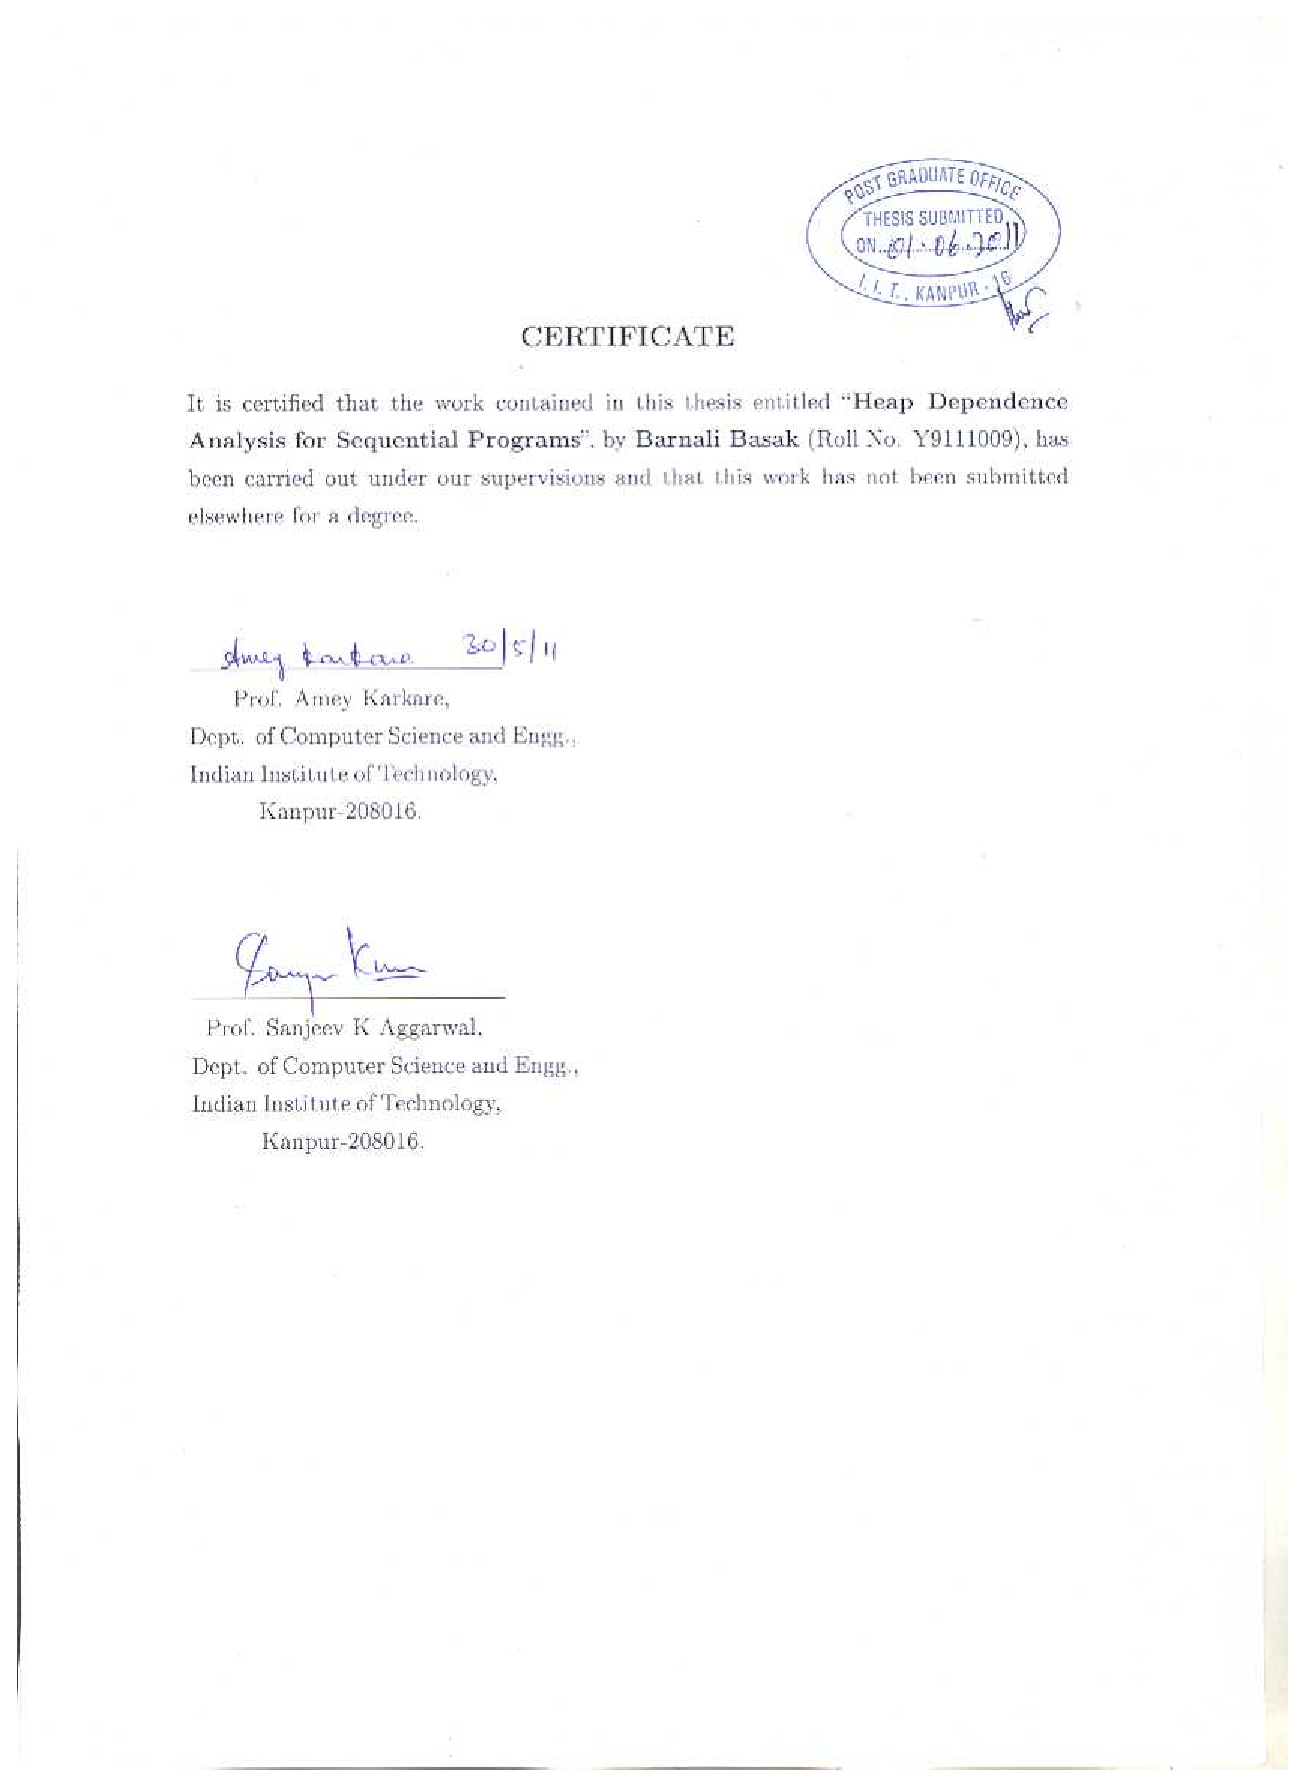
\includegraphics[width=\textwidth]{barnali.eps}
\vspace{2in}
\begin{abstract}
Identifying dependences present in the body of sequential 
program is used by parallelizing compilers to 
automatically extract parallelism from the program. 
Dependence detection mechanisms for programs with scalar 
and static variables is well explored and have become a 
standard part of parallelizing and vectorizing compilers. 
However, detecting 
dependences in the presence of dynamic (heap) recursive 
data structures is highly complex because of the unbound and dynamic nature of 
the structure. 
The problem becomes more critical due to the presence of pointer-induced aliasing . 

This thesis addresses the aforementioned problem and gives a  
novel approach for dependence analysis of sequential programs 
in presence of heap data structure.  
The novelty of our technique lies in the two-phase mechanism, 
where the first phase identifies dependences for whole procedure. 
It computes abstract 
{\em heap access paths} for each heap accessing statement 
in the procedure. The access paths approximate the locations accessed 
by the statement. For each pair of statements these access paths are 
checked for interference. 
The second phase refines the dependence analysis in the context of 
loops. The main aspect of the second phase is the way we convert 
the precise access paths, for each statement, into equations
that can be solved using traditional tests, e.g. GCD test, and 
Lamport test. The technique discovers {\em loop dependences}, 
i.e. the dependence among two different iterations of the same 
loop. Further, we extend the intra-procedural analysis to inter-procedural one. 
\end{abstract} 
 
%\newpage
\begin{center}
\thispagestyle{empty}
\vspace*{2in}
{\it This thesis is dedicated\\
to my parents and my beloved friend.}
\end{center}
\chapter*{Acknowledgment}
\vspace{1.0in}
I would like to express my heartiest gratitude towards my thesis supervisor {\bf Professor Amey Karkare}
 for his invaluable support and encouragement. His guidance has helped
me from initial till the final level of this work on the way developing a sound
understanding of the topic. It would have been very difficult for me to complete
this work without his innumerable innovative suggestions, the freedom that he has
provided and his utmost patience in hearing my problems out. Apart from gaining a lot from 
his huge technical expertise, starting from gaining tips about how to write a good report to 
getting insights whenever I got struck, I got many learnings which I will explore throughout my life. \\
%%
I wish to thank {\bf Prof. Sanjeev K. Aggarwal}, for his 
immense support and invaluable suggestions 
that I have received from him. \\
I would also like to thank {\bf Prof. Subhajit Roy} for 
all the enriching discussions that I had with him.\\
%%
%In the preparation of this report, I had to consult constantly 
%various papers, articles and journals. I, hereby, acknowledge 
%my indebtedness to them all. \\
%%
Special thanks to my friend and fellow mate 
{\bf Ms. Barnali Basak} for her encouragement and enormous 
help and lots of thanks to my institution without which this 
thesis would have been a distant reality. \\
%%
Finally, I wish to extend my thanks to my parents, my sister and my beloved 
friends, who have always been a source of inspiration 
and encouragement. Their love and blessings have always 
been a driving force in my life to carry all my works 
with hope and optimism.\\
%%
Every effort has been made to give credit where it is due for
the material contained here in. If inadvertently I have
omitted giving credit to anyone, I apologize and express my
gratitude for their contribution to this work. 
\begin{flushright} \large
\textit{Sandeep Dasgupta}\\
\textit{June 2011}\\
\textit{Indian Institute of Technology, Kanpur}\\
\end{flushright}
\newpage

\pagenumbering{roman}
\tableofcontents
\listoffigures
\listoftables
%\newpage
%\newenvironment{mydef}[1]{\begin{definition} #1 \mbox{\\}
%\rm}{\end{definition}}
\pagenumbering{arabic}
\chapter{Introduction}
\label{ch:Intro}
In the recent arena of parallel architectures (multi-cores,
GPUs, etc.), software side lags behind hardware. This is due to the reason that dealing with 
parallelism adds a new dimension to the design of programs, therefore 
makes it complex. One approach for efficient parallelization of programs is to explicitly 
induce parallelism. It includes designing of concurrent programming languages like Go, X10 etc., 
libraries, APIs like POSIX, OpenMP, Message 
Passing Interface(MPI) etc. The main advantage of such approach is that it gives simple and clear directions to the 
compiler to parallelize the code. But the main drawbacks of such approach is that the degree of parallelism totally depends upon 
the efficiency of programmer and imposing external parallelism turns the code into legacy one. 
The other approach is to automatically 
parallelizing sequential programs by compiler which extract parallelism 
without violating correctness. This is a key step in increasing
the performance and efficiency. 
%
\section{Motivation}
Over the past years, lot of work has been done on automatically 
parallelizing sequential programs. These approaches have mainly 
been developed for programs having only static data structures 
(fixed sized arrays) and written in languages such as FORTRAN
~\cite{Allen87automatic,Banerjee93automatic,Wolf91loop,
  Kennedy01Optimizing}. Almost all programming languages
today use the heap for dynamic recursive data structures. 
\begin{comment}
The basic building block of such structure is node which consists 
of one or more fields. Each field is designated as a scalar field or 
pointer field. A pointer field contains either \emph{null} value or pointer to 
a node of the same type. 
\end{comment}

Therefore, any parallelization must also take into account the data
dependency due to the access of common heap nodes of such 
structures. Finding parallelism in sequential programs written
in languages, with dynamically allocated data structures, such
as C, C++, JAVA, LISP etc., has been less successful. One of
the reason being the presence of pointer-induced aliasing,
which occurs when multiple pointer expressions refer to same
storage location. Compared to the analysis of static and
stack data, analyzing properties of heap data is challenging
because the structure of heap is unknown at compile time. It
is also potentially unbounded and the lifetime of a heap
object is not limited by the scope that creates it. As a
consequence, properties of heap (including dependence) are
approximated very conservatively. The approximation of the
heap data dependence information inhibits the parallelization. 

The objective of our analysis is to detect both coarse-grained parallelism 
in the context of function calls, loops and fine-grained parallelism in the 
context of statements. We show the following two examples as motivating 
examples of our work.
\begin{figure}[t]
  \begin{center}
  
    \scalebox{.85}{\begin{tabular}{ c | c }
%    \hline
 	& \multirow{3}{*}{ {\tt
\begin{program}{0}
%  \FL\ \ldots
  \UNL{0} void treeAdd(tree t) \{
  \UNL{1}  if(t == NULL)
  \UNL{2} return;
  \NL{1}     tl = t$\rightarrow$left;
  \NL{1}     treeAdd(tl);
  \NL{1}     tr = t$\rightarrow$right;
  \NL{1}     treeAddd(tr);
  \UNL{1}	t\rtarrow{num} = tl\rtarrow{num} + tr\rtarrow{num};
  \UNL{0} \}
\end{program}
}} \\
%    & \\
      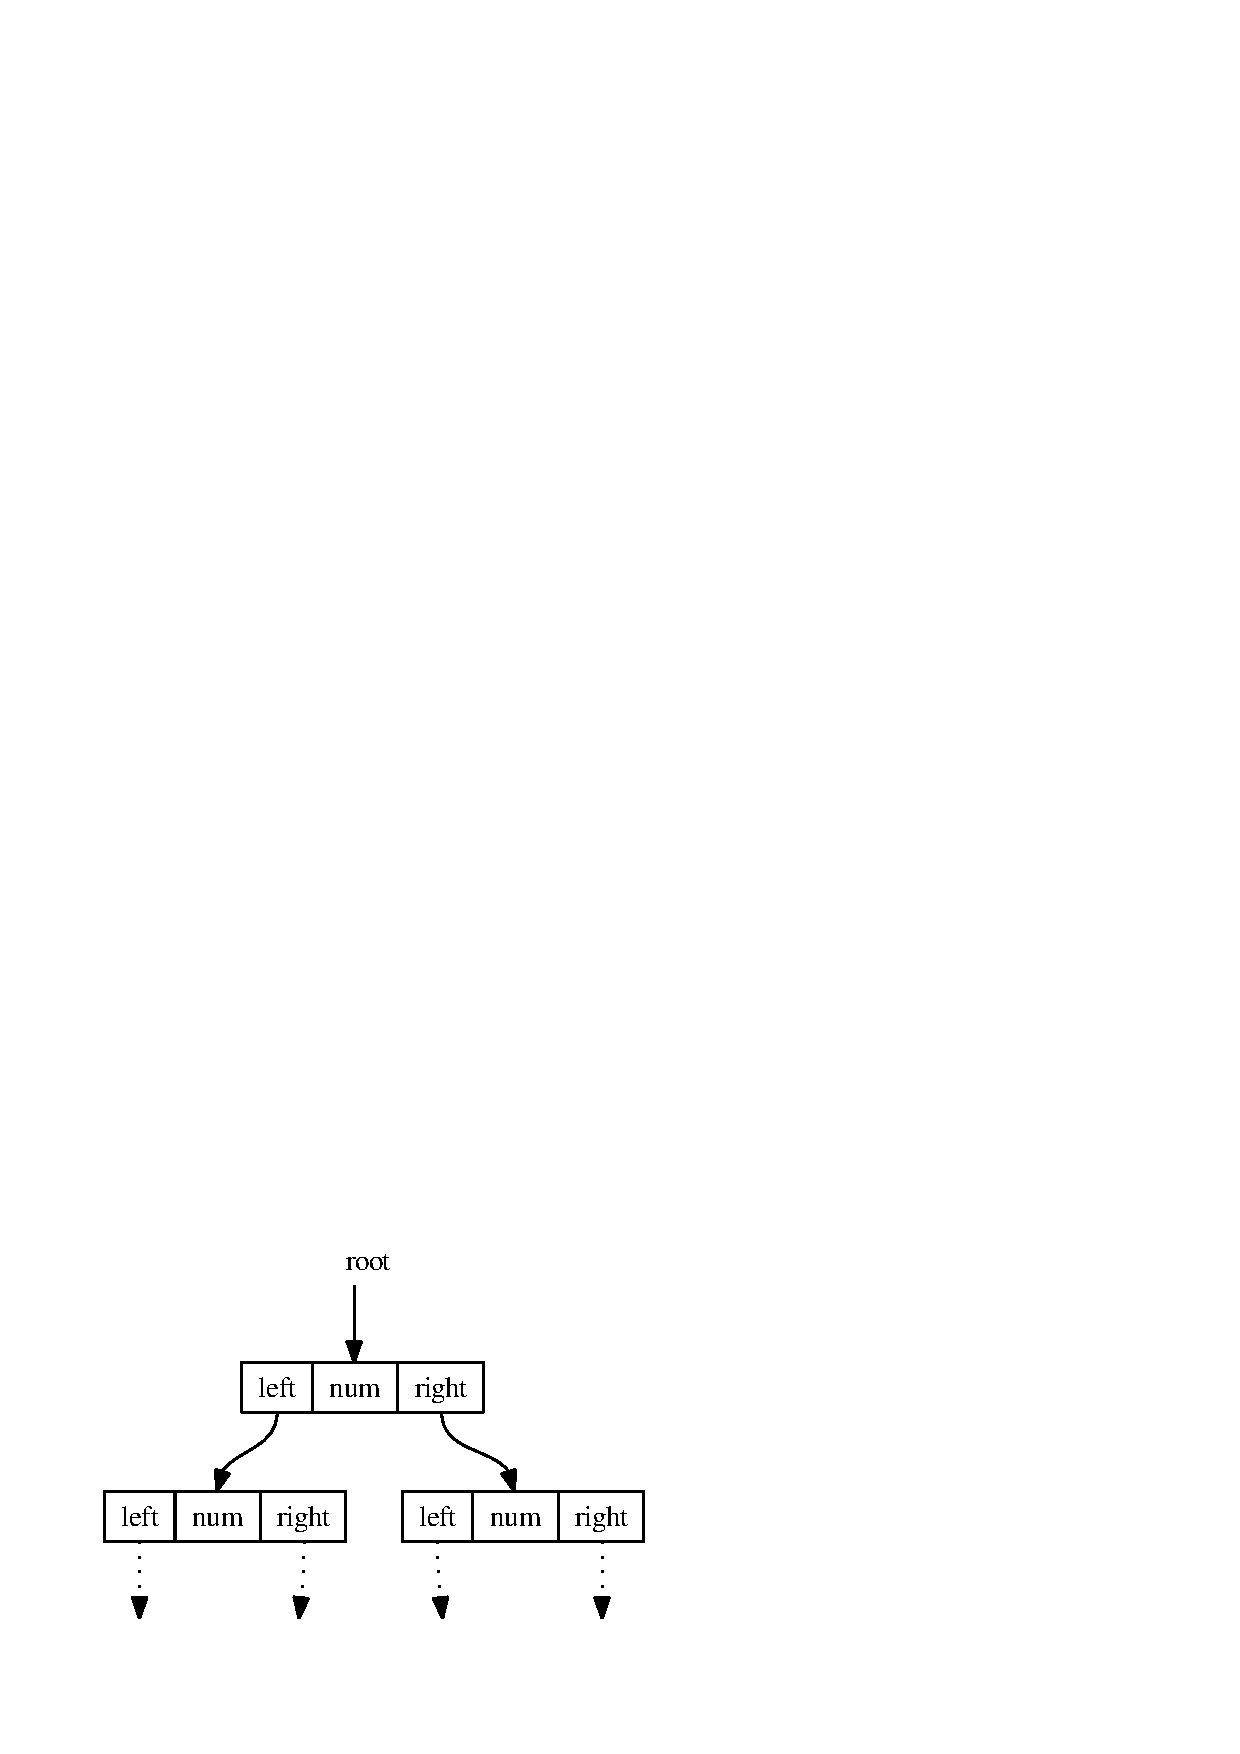
\includegraphics[scale=0.6]{tree_grph}
      & \\
%      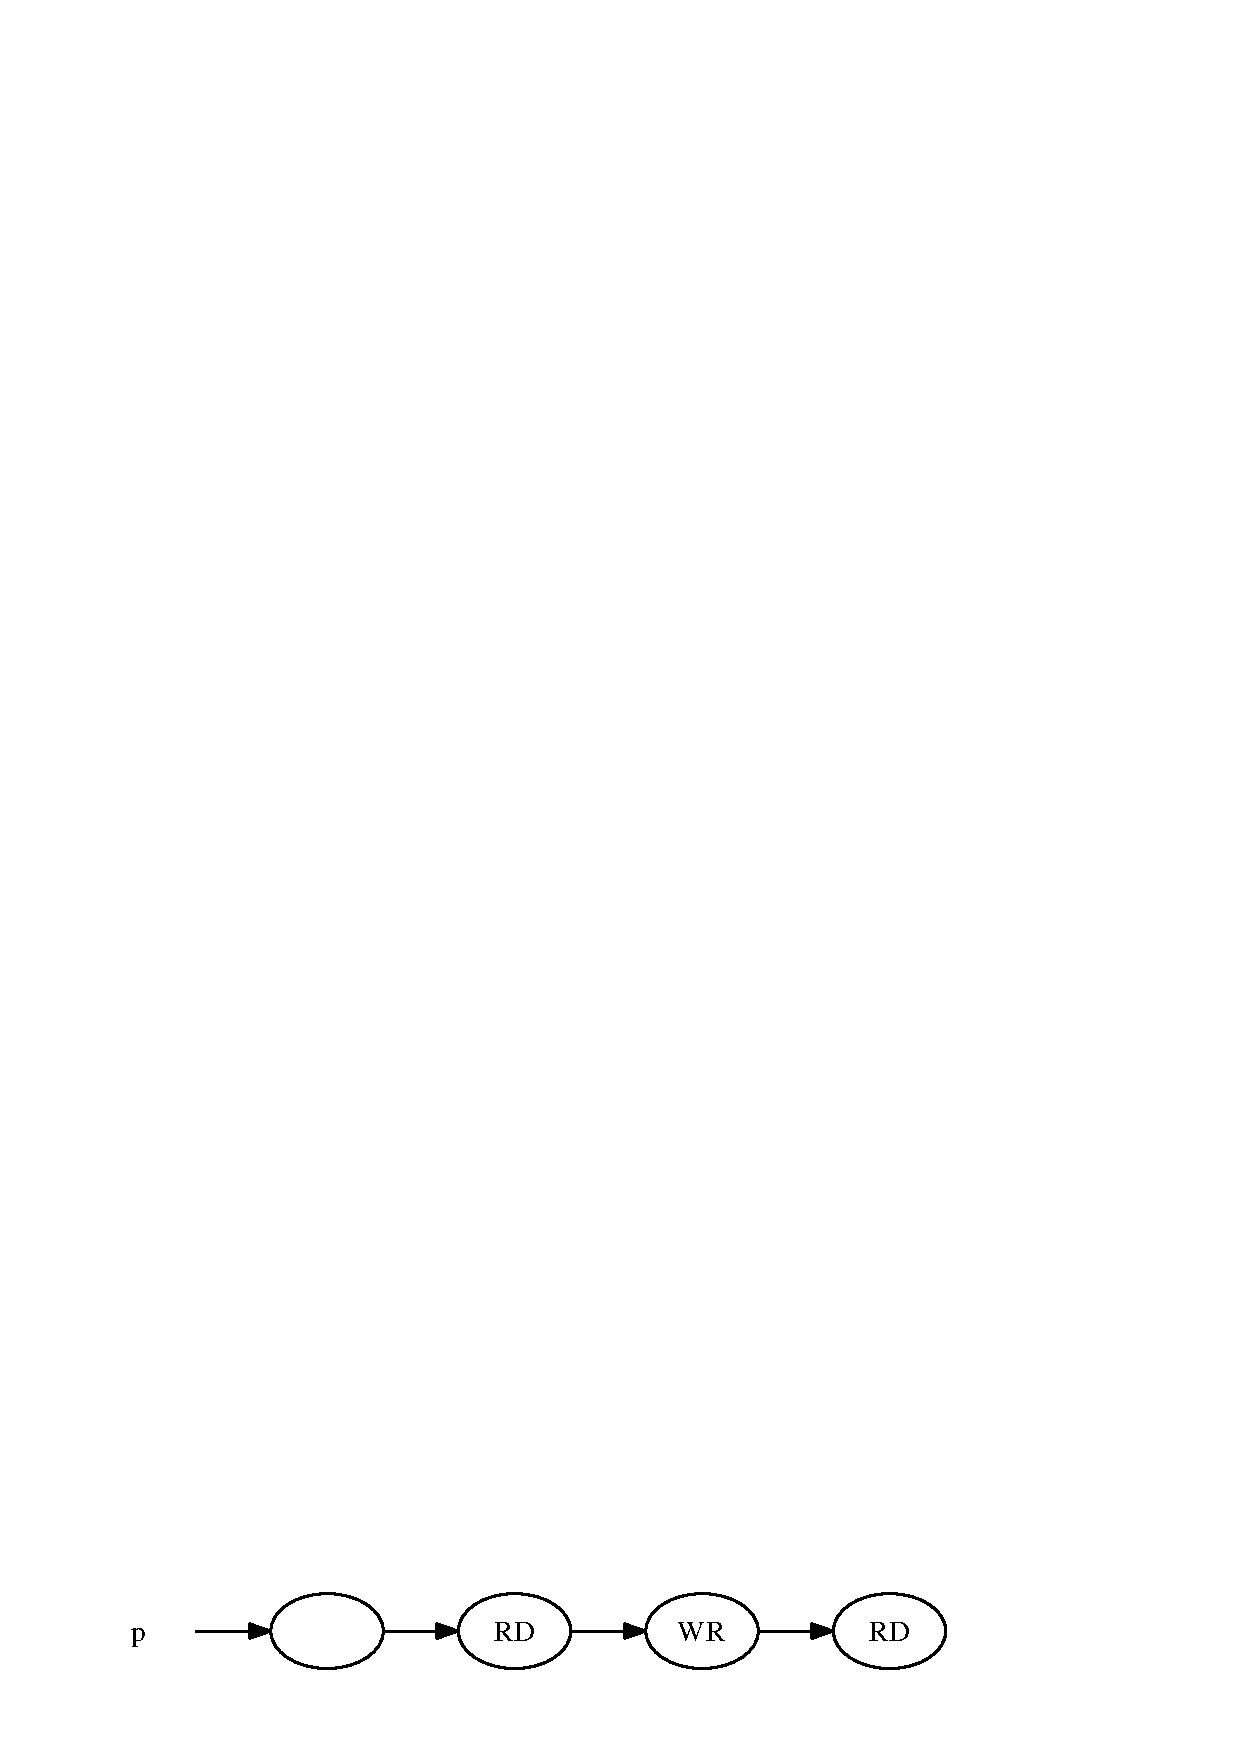
\includegraphics[scale=0.6]{grph_motiv} & \\
%      (a) & (b) \\
     (a) Data structure & 
     (b) Function traversing the data structure. \\
%    \hline 
    \end{tabular}}
  \end{center}
  \hrule
  \caption{\label{fig:motiv1} Motivating example: function-call parallelization}
%\hrule
\end{figure}
\begin{example}{\rm 
Consider Figure~\ref{fig:motiv1} which gives a motivational 
example for parallelism in the context of function calls. It shows 
the tree data 
structure and the function \emph{treeAdd} traversing on the 
data structure. In the code fragment the two calls to the function 
\emph{treeAdd} respectively perform the additions of left and right 
subtrees recursively. If the analysis can ensure that the two function calls 
do not access any common region of heap, they can be executed in parallel.
} 
\hfill\psframebox{}  
\end{example}
%%%%%%%%%%%%%%%%%
\begin{figure}[t]
  \begin{center}
  
    \scalebox{.85}{\begin{tabular}{ c | c }
 %   \hline
      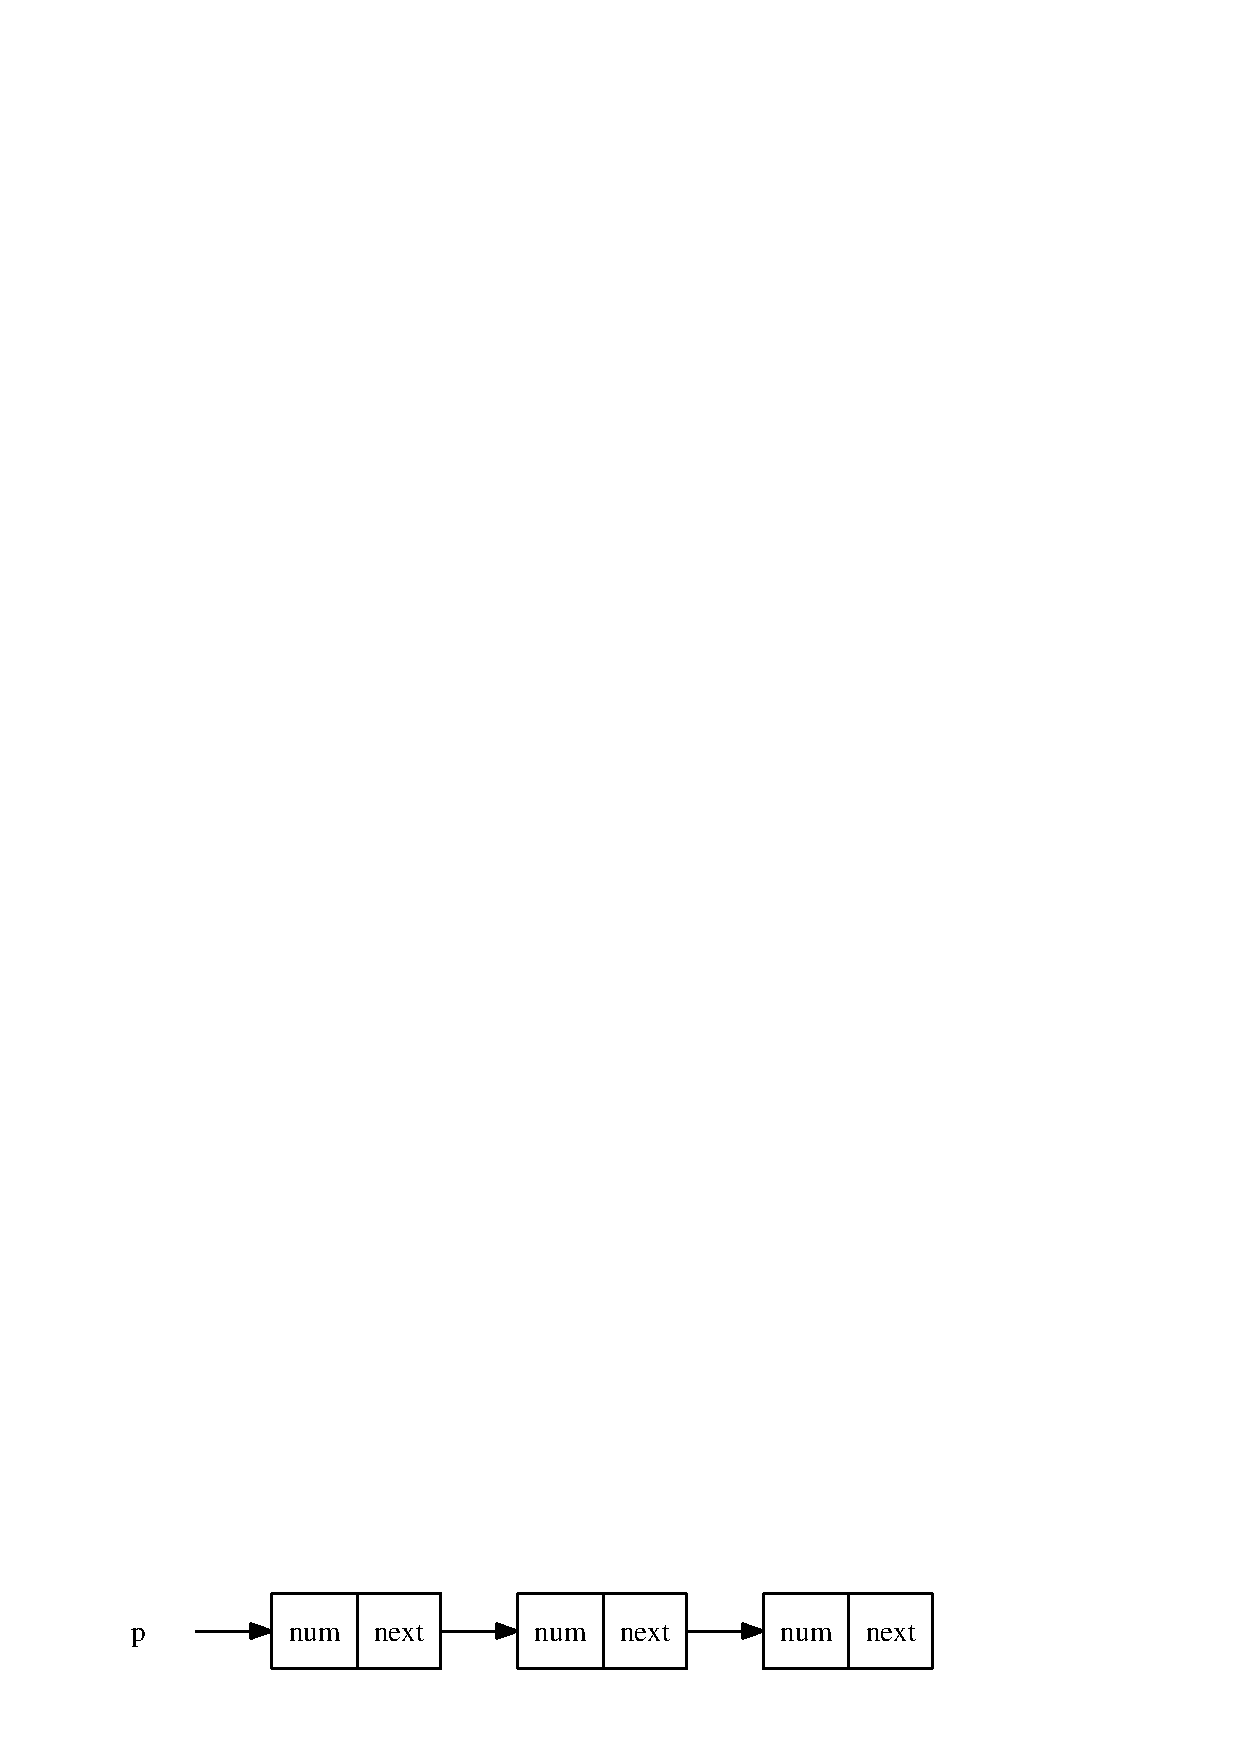
\includegraphics[scale=0.6]{grph4} %\cline{1-1}
      &
      {\tt
\begin{program}{0}
  \FL\ \ldots
  \NL{0} p = list;
  \UNL{0} \WHILE (p$\rightarrow$next != NULL) \{
  \NL{1}     q = p$\rightarrow$next;
  \NL{1}     temp = q$\rightarrow$num;
  \NL{1}     r = q$\rightarrow$next;
  \NL{1}     r$\rightarrow$num = temp;
  \NL{1}     p = r;
  \UNL{0} \}
  \UNL{0} \ldots
\end{program}
} \\
      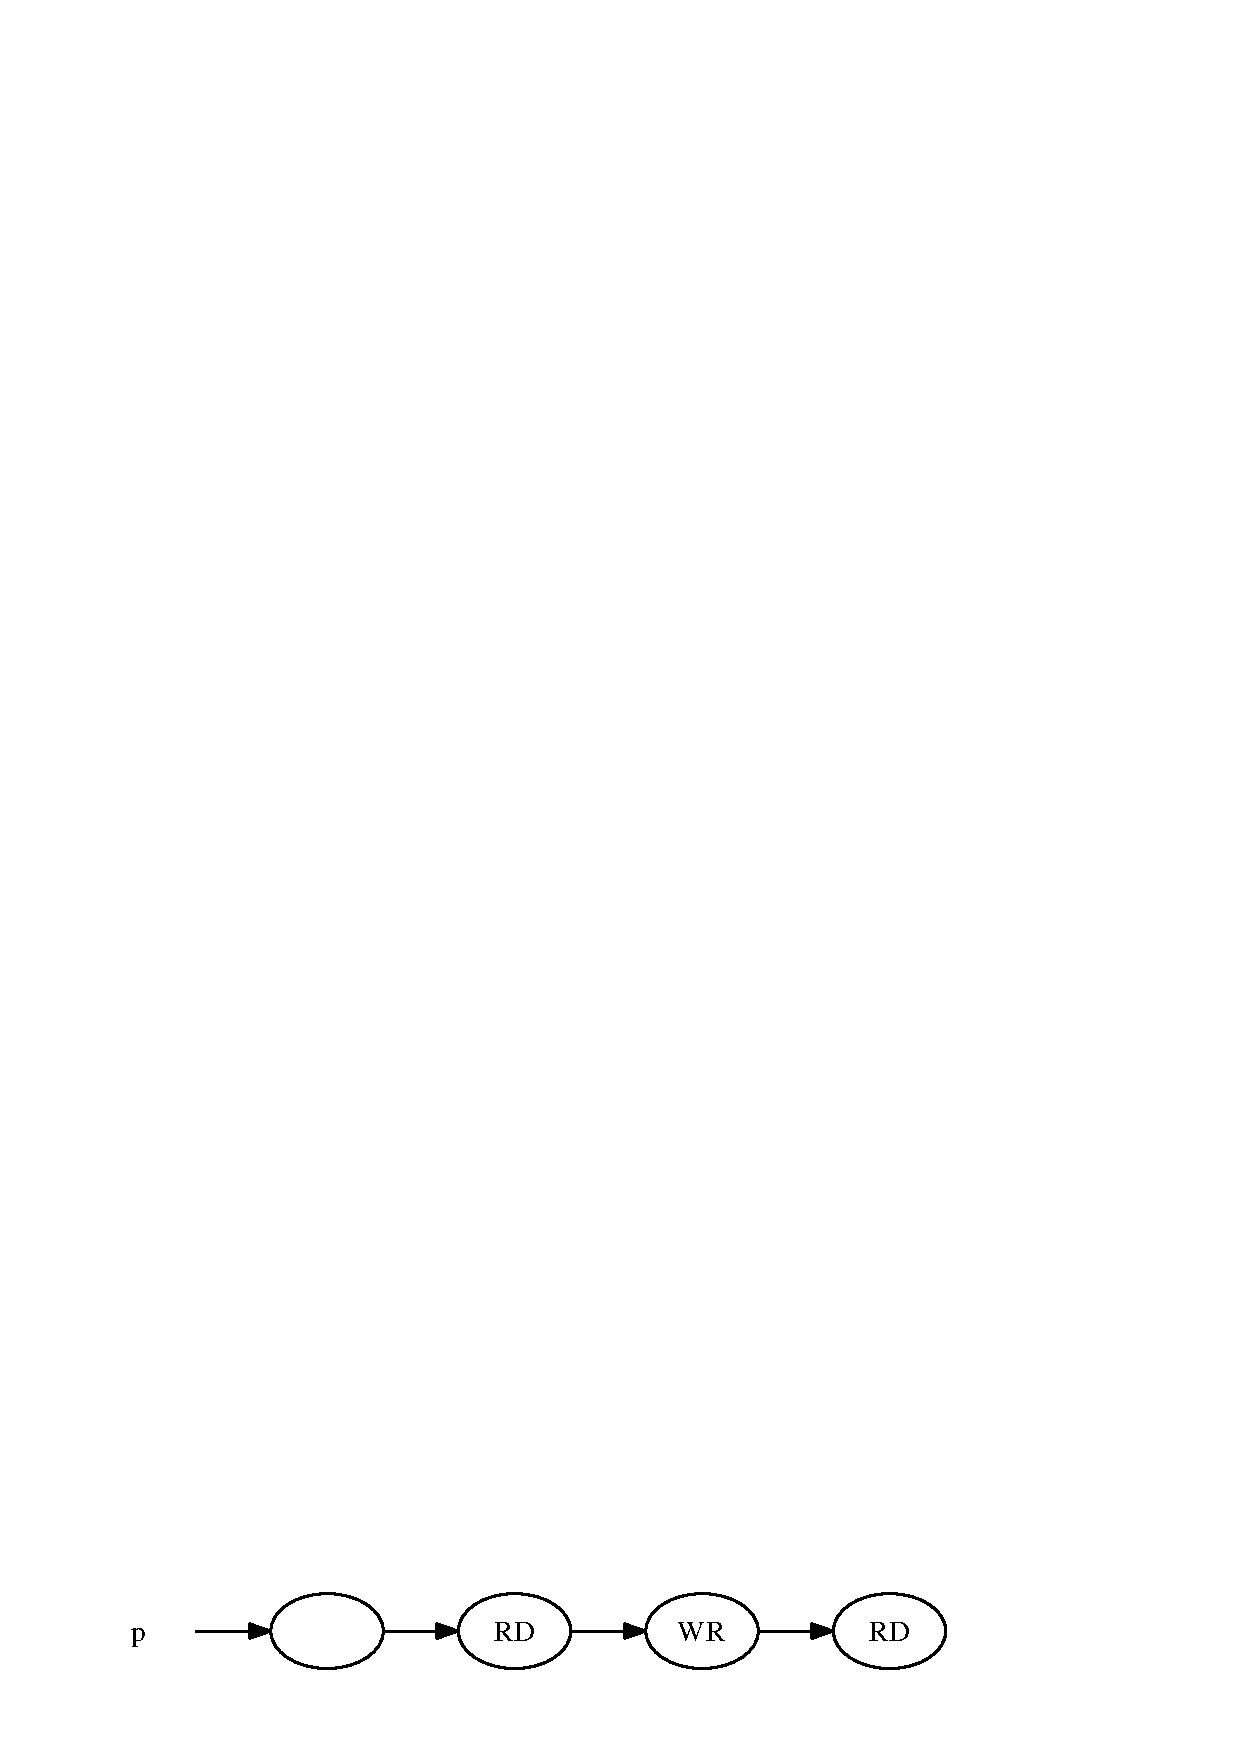
\includegraphics[scale=0.6]{grph_motiv} & \\
%      (a) & (b) \\
     (a) Nodes read and written by code & 
     (b) Loop traversing the data structure. \\
    \end{tabular}}
  \end{center}
  \hrule
  \caption{\label{fig:motiv} Motivating example: loop parallelization}
%\hrule
\end{figure}
\begin{example}{\rm
  Figure~\ref{fig:motiv}
  shows an example of loop level parallelism. It shows list data structure and the nodes of the structure being read and written, tagged by \emph{Read} (\ttf{RD}) 
  and \emph{Write} (\ttf{WR}) access by the code fragment traversing the
  data structure. Note that, the first node of the structure is a special node which is neither 
  read nor written by the code fragment. The performance of the code can be improved if the loop can
  be executed in parallel. However, without the knowledge of
  precise heap dependences, we have to assume worst case
  scenario, i.e.,  the  location read by the statement {\tt
    S3} in some iteration could be the same as the location
  written by the statement {\tt S5} in some other iteration.
  In that case,  it is not possible to parallelize the loop.
 
  Our dependence analysis can show that the locations read by
  {\tt S3} and those written by {\tt S5} are mutually
  exclusive. Further, it also shows the absence of any other
  dependences.  This information, along with the information
  from classical control and data dependence analysis, can be
  used by a parallelizing compiler to parallelize the loop.
}
\hfill\psframebox{}  
\end{example}

This report explains our approach for a practical heap data dependence analysis. 
As it is understood that we are only talking about data dependences, we drop the term 
data in the rest of the report. 
%
\section{Contributions of our Work}
Our work contributes in the area of heap based 
dependence analysis. We present a novel approach 
which identifies dependences and extracts parallelism for a sequential program. 
In particular, our approach finds out dependences between two statements. 
This enables us to find out whether two procedure calls 
access disjoint structures, hence can be executed in parallel. 
Then we refine this technique to work better 
in presence of loops. We also extend the work of loop analysis 
for static and scalar data to support heap intensive loops.

\section{Organization of the Thesis}
The rest of the thesis is organised as follows. We discuss about related 
work done in the field of heap intensive dependence analysis in Chapter~\ref{ch:RelatedWork}.
Chapter~\ref{ch:back} specifies the imperative programming model 
for which our analysis is defined and gives the other background 
details. Chapter~\ref{ch:dep} through~\ref{ch:interdep} provide a complete 
description of our practical dependence analysis applied to 
dynamically allocated structure. Chapter~\ref{ch:dep} gives the detailed 
explanation of the intra-procedural dependence detection technique 
which separately works on each procedure of a program. Chapter~\ref{ch:loopdep} 
presents our method to handle loops in a more specific way. We also 
give the inter-procedural framework for our analysis in Chapter~\ref{ch:interdep}. 
Chapter~\ref{ch:result} demonstrates our whole method by extensively 
analysing few benchmark codes. We conclude the report in Chapter~\ref{ch:conclusion} 
by giving the direction for future research.
\chapter{Related Work} \label{ch:RelatedWork}
The shape-analysis problem was initially studied in the
context of functional languages. Jones and
Muchnick~\cite{Jones79} proposed one of the earliest shape
analysis technique for Lisp-like languages with destructive
updates of structure. They used sets of finite shape graphs
at each program point to describe the heap structure.  To
keep the shape graphs finite, they introduced the concept of
$k$-limited graphs where all nodes beyond $k$ distance from
root of the graph are summarized into a single node. Hence
the analysis resulted in conservative approximations. The
analysis is not practical as it is extremely costly both in
time and space .

Chase et al.~\cite{Chase90} introduced the concept of limited
reference count to classify heap objects into different
shapes. They also classified the nodes in concrete and
summary nodes, where summary nodes were used to guarantee
termination. Using the reference count and concreteness
information of the node, they were able to kill relations
({\em strong updates}) for assignments of the form $\p\rightarrow f = \q$
in some cases. However, this information is not
insufficient to compute precise shape, and detects false
cycle even in case of simple algorithms like destructive list
reversal.

Sagiv et. al.~\cite{Sagiv96,Sagiv99,Sagiv02toplas} proposed
generic, unbiased shape analysis algorithms based on {\em
  Three-Valued} logic. They introduce the concepts of {\em
  abstraction} and {\em re-materialization}. Abstraction is
the process of summarizing multiple nodes into one and is
used to keep the information bounded.  Re-materialization is
the process of obtaining concrete nodes from summary node and
is required to handle destructive updates. By identifying
suitable predicates to track, the analysis can be made very
precise.  However, the technique has potentially exponential
runtime in the number of predicates, and therefore not
suitable for large programs.


Distefano et al.~\cite{distefano06local} presented a shape
analysis technique for linear data structures (linked-list
etc.), which works on symbolic execution of the whole program
using separation logic. Their technique works on suitable
abstract domain, and guarantees termination by converting
symbolic heaps to finite canonical forms, resulting in a
fixed-point. By using enhanced abstraction scheme and
predicate logic, Cherini et al.~\cite{cherini10shape}
extended this analysis to support nonlinear data structure
(tree, graph etc.).

Berdine et al.~\cite{berdine07shape} proposed a method for
identifying composite data structures using generic
higher-order inductive predicates and parameterized spatial
predicates.  However, using of separation logic does not
perform well in inference of heap properties.  Hackett and
Rugina in~\cite{hackett05region} presented a new approach for
shape analysis which reasons about the state of a single heap
location independently. This results in precise abstractions
of localized portions of heap. This local reasoning is then
used to reason about global heap using context-sensitive
inter-procedural analysis.  Cherem
et. al.~\cite{cherem07doubly} use the local abstraction
scheme of~\cite{hackett05region} to generate local invariants
to accurately compute shape information for complex data
structures.  

Jump and McKinley~\cite{maria09dynamic} give a technique for
dynamic shape analysis that characterizes the shape of
recursive data structure in terms of dynamic degree metrics
which uses in-degrees and out-degrees of heap nodes to
categorize them into classes. Each class of heap structure is
then summarized. While this technique is useful for detecting
certain types of errors; it fails to visualize and understand
the shape of heap structure and cannot express the sharing
information in general.

Our work is closest to the work proposed by Ghiya
et. al.~\cite{Ghiya96} and by Marron
et. al.~\cite{marron06static}.  Ghiya et al.~\cite{Ghiya96}
keeps interference and direction matrices between any two
pointer variables pointing to heap object and infer the shape
of the structure as Tree, DAG or Cycle. They have also
demonstrated the practical applications of their
analysis~\cite{Ghiya96practicaltechniques,Ghiya98a,Ghiya98b} and shown that it works well on practical
programs. However, the main shortcoming of this approach is
it cannot handle kill information. In particular, the
approach is unable to identify transitions from Cycle to DAG,
from Cycle to Tree and from DAG to Tree. So it has to to
conservatively identify the shapes.

Marron et. al.~\cite{marron06static} presents a data flow
framework that uses heap graphs to model data flow
values. They presented an abstract heap model that can represent 
information on aliasing, shape, logical data structures, sharing between variables, 
and sharing between data elements in collections.
They introduce a restricted version of refinement, based on the ideas presented by Sagiv,
Reps and Wilhelm. Using this restricted notion of refinement, they demonstrate how this 
model can be used to accurately simulate important program events such as list copying, sorting, reversal,
and various other destructive operations. 
The analysis uses technique similar to
re-materialization, but unlike parametric shape analysis
techniques~\cite{Sagiv99,Sagiv02toplas}, the
re-materialization is approximate and may result in loss of
precision. 

Our method is also data flow analysis framework, that uses
matrices and boolean functions as data flow values. We use
field sensitive connectivity matrices to store path
information, and boolean variables to record field
updates. By incorporating field sensitivity information, we
are able to improve the precision without much impact on
efficiency. The next chapter presents a simplified view of
our approach before we explain it in full details.

As our work is closest to the work of Ghiya
et. al.~\cite{Ghiya96} we present a brief summary of their
analysis in Appendix A.

\cmt{
%%%%%%%%%%%%%%%%%%%%%%%%%%%%%%%%%%%%%%%%%%%%%%%%%%%%%%%%%%%%%%%%%%%%%%
\section[Analysis of Ghiya et. al.~\cite{Ghiya96}]{Analysis of Ghiya et. al.~\cite{Ghiya96}\footnote{The contents of this section are borrowed from ~\cite{Ghiya96}}}
%%%%%%%%%%%%%%%%%%%%%%%%%%%%%%%%%%%%%%%%%%%%%%%%%%%%%%%%%%%%%%%%%%%%%%
Their shape analysis composed of three store-less
abstractions that are computed together at each program point.
For each heap directed pointer they approximated the attribute
shape and for each pair of heap directed pointers they approximated the 
direction and interference relationships between them. These three abstractions 
are defined formally as follows:

\begin{definition}
Given any heap-directed pointer $p$, the shape attribute p.shape is Tree, 
if in the data structure accessible from p there is a unique (possibly empty) access path 
between any two nodes (heap objects) belonging to it. It is considered to be DAG (directed acyclic graph), 
if there can be more than one path between any two nodes in this data structure, 
but there is no path from a node to itself (i. e, it is acyclic). 
If the data structure contains a node having a path to itself, p.shape is considered to be Cycle.
Note that as lists are special case of tree data structures, their shape is also considered as Tree.
\end{definition}

\begin{definition}
Given two heap directed pointers $p$ and $q$, the direction matrix $D$ captures the following 
relationships between them:
\begin{itemize}
\item $D[p,q] = 1 : $ An access path possibly exists in the heap, from the heap object pointed to by $p$,
to the heap object pointed to by $q$. In this case we simply say that the pointer $p$ has a path to 
pointer $q$.
\item $D[p,q] = 0 : $ No access path exists from the heap object pointed to by $p$ to the heap object pointed to by $q$. 
\end{itemize}
\end{definition}

\begin{definition}
Given two heap directed pointers $p$ and $q$, the direction matrix $I$ captures the following 
relationships between them:
\begin{itemize}
\item $I[p,q] = 1 : $ A common heap object can be possibly accessed starting from pointers $p$ and $q$.
In this case we state that pointers $p$ and $q$ can interfere.
\item $I[p,q] = 0 : $ No common heap object can be accessed starting from pointers $p$ and $q$.
In this case we state that pointers $p$ and $q$ do not interfere.
\end{itemize}
\end{definition}

Direction relationships are used to actually estimate the shape attributes, where the interference 
relationships are used for safely calculating direction relationships. 

\subsection{Illustrative Example}

The direction and interference matrices are illustrated in Fig.~\ref{fig:relwork_1}.
Part (a) represents a heap structures at a program point, while parts (b) and (c) show the direction 
and interference matrices for it.  
\begin{figure}
\centering
\begin{tabular}{c@{$\qquad\qquad$}c}
\multicolumn{2}{c}{
\scalebox{0.80} { 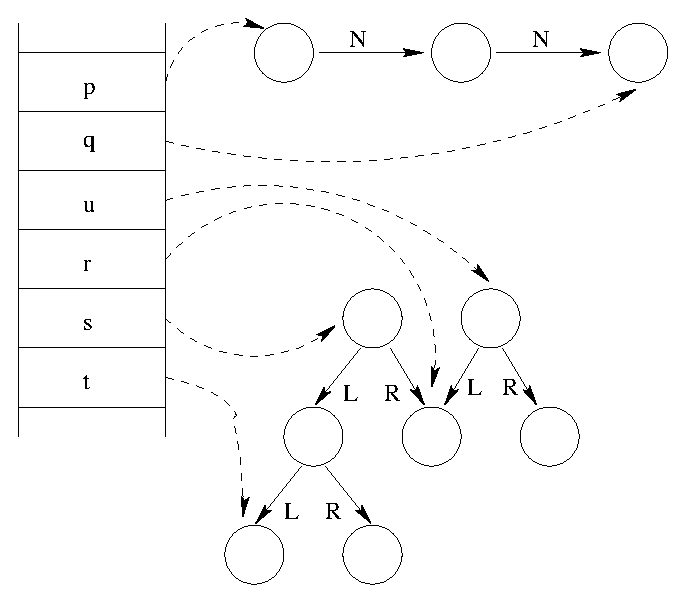
\includegraphics[scale=1]{diagrams/Appendix_2.eps}}
} \\
\multicolumn{2}{c}{
\scalebox{0.80}{ (a) Heap Structure }
} \\ \\
\scalebox{0.80} { \begin{tabular}{|c||c|c|c|c|c|c|}
\hline
$D$ & $p$ & $q$ & $r$ & $s$ & $t$ & $u$ \\ \hline \hline
$p$ & $1$ & $1$ & $0$ & $0$ & $0$ & $0$ \\ \hline 
$q$ & $0$ & $1$ & $0$ & $0$ & $0$ & $0$ \\ \hline 
$r$ & $0$ & $0$ & $1$ & $0$ & $0$ & $0$ \\ \hline 
$s$ & $0$ & $0$ & $1$ & $1$ & $1$ & $0$ \\ \hline 
$t$ & $0$ & $0$ & $0$ & $0$ & $1$ & $0$ \\ \hline 
$u$ & $0$ & $0$ & $1$ & $0$ & $0$ & $1$ \\ \hline 
\end{tabular}} 
& 
\scalebox{0.80} {\begin{tabular}{|c||c|c|c|c|c|c|}
\hline
$I$ & $p$ & $q$ & $r$ & $s$ & $t$ & $u$ \\ \hline \hline
$p$ & $1$ & $1$ & $0$ & $0$ & $0$ & $0$ \\ \hline 
$q$ & $1$ & $1$ & $0$ & $0$ & $0$ & $0$ \\ \hline 
$r$ & $0$ & $0$ & $1$ & $1$ & $0$ & $1$ \\ \hline 
$s$ & $0$ & $0$ & $1$ & $1$ & $1$ & $1$ \\ \hline 
$t$ & $0$ & $0$ & $0$ & $1$ & $1$ & $0$ \\ \hline 
$u$ & $0$ & $0$ & $1$ & $1$ & $0$ & $1$ \\ \hline 
\end{tabular}}  \\
\scalebox{0.80}{ (b) Direction Matrix}  & \scalebox{0.80} {(c) Interference Matrix}
\end{tabular}
\caption{Example Direction and Interference Matrices}
\label{fig:relwork_1}
\end{figure}


We now demonstrate how direction relationships help estimate the shape of the data structures.
In Fig.~\ref{fig:relwork_2}, initially we have both \p.\shape\ and \q.\shape\ as Tree. Further $D[q,p] == 1$, as there 
exists a path from \q\ to \p\ through {\tt next} link. The statement {\tt p$\rightarrow$prev = q}, sets up a path from
\p\ to \q\  through the {\tt prev} link. From direction matrix information we already know that a path exists
from \q\ to \p, and now a path is being set from \p\ to \q. Thus after the statement, $D[p,q] = 1$, $D[q,p] = 1$, \p.\shape\ = Cycle
and \q.\shape\ = Cycle.  

\begin{figure}
\centering
\scalebox{.80} {
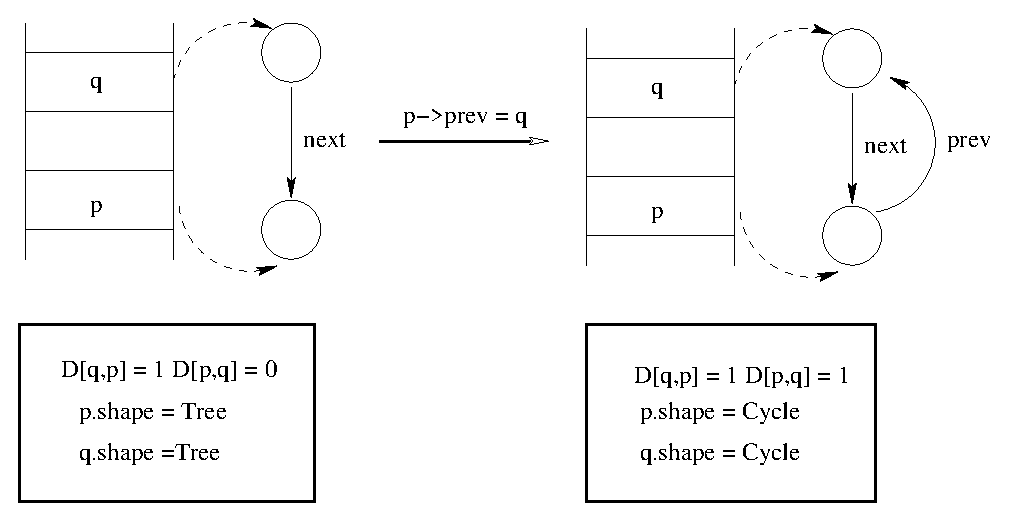
\includegraphics[scale=1]{Figure/figure_3}
}
\caption{Example Demonstrating Shape Estimation}
\label{fig:relwork_2}
\end{figure}

\subsection{Analysis of Basic Statements}
They have considered eight basic statements that can access or
modify heap data structures as listed in Fig.~\ref{fig:relwork_3}(a). Variables \p\ and \q and the field $f$ are
of pointer type, variable $k$ is of integer type, and $op$ denotes the $+$ and $-$ operations. The 
overall structure of the analysis is shown in Fig.~\ref{fig:relwork_3}(b). Given the direction and the interference 
matrices $D$ and $I$ at a program point x, before the given statement, they compute the matrices $D_n$ and $I_n$
at a program point y. Additionally, we have the attribute matrix A, where for a pointer $p$, $A[p]$ gives its shape attribute.
The attribute matrix after the statement is presented as $A_n$.

For each statement they compute the set of direction and interference relationships it kills and generates. Using these sets, the
new matrices $D_n$ and $I_n$ are computed as shown in Fig.~\ref{fig:relwork_3}(c). Note that the elements in the gen and kill sets are denoted as $D[p,q]$
for direction relationships, and $I[p,q]$ for interference relationships. Thus a gen set of the form $\{D[x,y], D[y,z]\}$, indicates that
the corresponding entries in the output direction matrix $D_n[x,y]$ and $D_n[y,z]$ should be set to one. We also compute the set of 
pointers $H_s$, whose shape  attribute can be modified by the given statement. Another attribute matrix $A_c$ is used to store the 
changed attribute of pointers belonging to the set $H_s$. The attribute matrix $A_n$ is then computed using the 
matrices $A$ and $A_c$ as shown in Fig.~\ref{fig:relwork_3}(c).  

Let $H$ be the set of pointers whose relationships/attributes are abstracted by the matrices $D$. $I$ and $A$. Further
assume that updating an interference matrix entry $I[\q,\p]$, implies identically updating the entry $I[\p,\q]$.   
\begin{figure}
\centering
\scalebox{0.90}{
\begin{tabular}{|c|c|c|}
\hline
\begin{tabular}{l}
Allocation \\
1. {\tt p = malloc();} \\
\\
Pointer Assignments \\
2. {\tt p = q;} \\
3. {\tt p = \&(q$\rightarrow$f);} \\
4. {\tt p = q op k;} \\
5. {\tt p = NULL;} \\
6. {\tt p = q$\rightarrow$f;} \\
\\
Structure Updates \\
7. {\tt p$\rightarrow$f = q;} \\
8. {\tt p$\rightarrow$f = NULL;}
\end{tabular}  &
\begin{tabular}{c}
\scalebox{0.80}{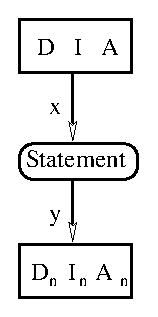
\includegraphics[scale=1]{diagrams/Appendix_4.eps}}
\end{tabular}
&
\begin{tabular}{l}
Build the new matrices\\
$\begin{array}{lll} 
\forall r,s \in H, & D_n[r,s] = D[r,s], & I_n[r,s] = I[r,s] \\
\forall s \in H, & A_n[s] = A[s]
\end{array}$ \\
\\
Delete Killed relationships \\
$\begin{array}{ll} 
\forall entries\ D[r,s] \in D\_kill\_set, & D_n[r,s] = 0\\  
\forall entries\ I[r,s] \in I\_kill\_set, & I_n[r,s] = 0\\  
\end{array}$ \\
\\
Add generated relationships \\
$\begin{array}{ll} 
\forall entries\ D[r,s] \in D\_gen\_set, & D_n[r,s] = 1\\  
\forall entries\ I[r,s] \in I\_gen\_set, & I_n[r,s] = 1\\  
\end{array}$ \\
\\
Update shape attributes of affected pointers \\
Compute $H_s$ and $A_s$ \\
$\begin{array}{ll} 
\forall s \in H_s, & A_n[s] = A[s]\\  
\end{array}$
\end{tabular}
\\
\scalebox{0.80}{(a) Basic statements} & \scalebox{0.80}{(b) Analysis Structure} & \scalebox{0.80}{(c) General Form of Analysis Rules} \\
\hline
\end{tabular}
}
\caption{The Overall Struture of the Analysis}
\label{fig:relwork_3} 
\end{figure}


The actual analysis rules can be divided into three groups: (1) allocations, (2) pointer assignments, and 
(3) structure updates. Figure~\ref{fig:relwork_4} shows the gen and kill sets corresponding to each statement. 
\begin{figure}[h]
\centering
\begin{tabular}{|l|c|}
\hline
1. {\tt p  = malloc();} &  
					$\begin{array}{lll}
						D\_kill\_set &=& \{D[p,s] \vert s \in H \wedge D[p,s]\}\ \cup\\
                                     &&   \{D[s,p] \vert s \in H \wedge D[s,p]\} \\
						I\_kill\_set &=& \{I[p,s] \vert s \in H \wedge I[p,s]\} \\
						D\_gen\_set &=& \{D[p,p]\} \quad I\_gen\_set = \{I[p,p]\} \\
						H_s &=& \{p\} \quad A_c[p] = Tree 	\\
					\end{array}$
								\\
\hline
\begin{tabular}{l}
2. {\tt p = q;} \\
3. {\tt p = \&(q$\rightarrow$f);} \\
4. {\tt p = q op k;} \\
\end{tabular}
 & 
				\begin{tabular}{l}
					Kill set same as that of {\tt p  = malloc();} \\
					$\begin{array}{lll}
						D\_gen\_set\_from &=& \{D[s,p] \vert s \in H \wedge s \not= p \wedge D[s,q]\} \\
						D\_gen\_set\_to &=& \{D[p,s] \vert s \in H \wedge s \not= p \wedge D[q,s]\} \\
						I\_gen\_set	&=& \{I[p,s] \vert s \in H \wedge s \not= p \wedge I[q,s]\}\ \cup \\
											&&  \{I[p,p] \vert I[q,q]\} \\
						D\_gen\_set	&=& D\_gen\_set\_from\ \cup D\_gen\_set\_to \\
						H_s &=& \{p\} \quad A_c[p] = A[q] 	\\
					\end{array}$
				\end{tabular}
								\\
\hline
5. {\tt p = NULL;} & 
				\begin{tabular}{l}
					Kill set same as that of {\tt p  = malloc();} \\
					$\begin{array}{lll}
						D\_gen\_set &=& \{\} \quad I\_gen\_set = \{\} \\
						H_s &=& \{p\} \quad A_c[p] = Tree 	\\
					\end{array}$
				\end{tabular}
								\\
\hline
6. {\tt p = q$\rightarrow$f;} & 
				\begin{tabular}{l}
					Kill set same as that of {\tt p  = malloc();} \\
					$\begin{array}{lll}
						D\_gen\_set\_from 	&=& \{D[s,p] \vert s \in H \wedge s \not= p \wedge I[s,q]\} \\
						D\_gen\_set\_to 	&=& \{D[p,s] \vert s \in H \wedge s \not= p \wedge s \not= q\ \wedge \\
                                            &&    D[q,s]\}\ \cup \{D[p,q] \vert A[q] = Cycle\}\ \cup \\
											&& \{D[p,p] \vert D[q,q]\} \\
						D\_gen\_set 		&=& D\_gen\_set\_from\ \cup D\_gen\_set\_to \\
						I\_gen\_set 		&=& \{I[p,s] \vert s \in H \wedge s \not= p \wedge I[q,s]\}\ \cup \\
											&&  \{I[p,p] \vert I[q,q]\} \\
						A_c[p] &=& A[q] 	\\
					\end{array}$
				\end{tabular}
								\\
\hline
7. {\tt p$\rightarrow$f = NULL;} & 
					$\begin{array}{lll}
						D\_kill\_set &=& \{\} \quad I\_kill\_set = \{\}\\
						D\_gen\_set 		&=& \{\} \quad I\_gen\_set  = \{\}\\
						A_c[p] &=& A[p]\ \forall p \in H  	\\
					\end{array}$
								\\
\hline
7. {\tt p$\rightarrow$f = q;} & 
				\begin{tabular}{l}
					Kill set same as that of {\tt p$\rightarrow$f = NULL;} \\
					$\begin{array}{lll}
						D\_gen\_set		&=& \{D[r,s] \vert r,s \in H \wedge D[r,p] \wedge D[q,s]\}  \\
						I\_gen\_set  	&=& \{I[r,s] \vert r,s \in H \wedge D[r,p] \wedge I[q,s]\} \\
					\end{array}$ \\ \\
					\underline{Pointer q already has a path to p, D[q,p] = 1} \\
					$\begin{array}{lll}
						H_s 			&=& \{s \vert s \in H \wedge (D[s,p] \vee D[s,q])\} \\
						D[q,p] &\Rightarrow& A_c[s] = Cycle\ \forall s \in H_s  	\\
					\end{array}$ \\ \\
					\underline{A[q] = Tree} \\
					$\begin{array}{lll}
						H_s 			&=& \{s \vert s \in H \wedge (D[s,p] \vee I[s,q])\} \\
						(\neg D[q,p] \wedge (A[q] = Tree)) &\Rightarrow& A_c[s] = A[s] \Join Dag\ \forall s \in H_s  	\\
					\end{array}$ \\ \\
					\underline{A[q] $\not=$ Tree} \\
					$\begin{array}{lll}
						H_s 			&=& \{s \vert s \in H \wedge D[s,p]\} \\
						(\neg D[q,p] \wedge (A[q] \not= Tree)) &\Rightarrow& A_c[s] = A[s] \Join A[q]\ \forall s \in H_s  	\\
					\end{array}$
				\end{tabular}
								\\
\hline							
\end{tabular}
\caption{Analysis Rules}
\label{fig:relwork_4}
\end{figure}

}


\section{Related Work}
It was for functional languages that first shape analysis was looked at. Jones and Muchnick~\cite{Muchnick79} 
suggested a method for finding shape of unbounded data objects in LISP like
languages using regular tree grammars. They associate with each program point a set of 
shape graphs and to handle termination of analysis they use k-limiting approach. So they treat all nodes
whose distance is more than k from root as a single summarized node. Due to its large consumption of space 
and time the analysis is not practical.

Chase et al.~\cite{Chase90}  has used the concept of heap reference counts. They associate each node with a reference 
count and then try to find that part of the heap where all nodes
have reference count as one, such portions are said to be a tree or list. 
They have tried to tackle the problems with k-limiting to some extent, however their work fails obtaining 
accurate results for recursive data structures.

Sagiv et al.~\cite{Sagiv99},~\cite{Sagiv02} have presented a family of abstract interpretation algorithms based on three-valued logic. 
They use abstraction, a method for summarizing node and to handle destructive updates they have 
come up with re-materialization which refers to the process of splitting summary nodes. An exponential number of shape nodes may arise because of
abstract interpretation, so its not suitable for practical purposes. Sagiv and Noam~\cite{SagivInter02} have also looked into inter procedural shape 
analysis for recursive programs but they work only on linked lists. 

The main idea of Brian et al.~\cite{hackett05region} is to  decompose heap abstractions and independently analyze different parts of the heap.
They also decompose memory abstraction horizontally and vertically. Now for the local work to propagate globally they proposed 
and used a context sensitive inter procedural shape analysis algorithm.

A dynamic shape analysis technique was proposed by Jump et al.~\cite{maria09dynamic}. They compute a class field 
summary graph that summarizes the dynamic object graph. This summary graph also records the in-degree and out-degree of each 
object which are the recursive degree metrics. In their analysis they keep track of those node which are of fixed degree and
also those whose degree is in a particular range. Since running the analysis after each pointer statement is very costly they 
do it by piggybacking with garbage collection. 

Susan et al.~\cite{sagivDemand95} have a polynomial worst case method for inter procedural analysis provided its a demand 
data flow analysis. It will determine whether a single given data flow value holds at some give point. But the class of problems 
it can handle was limited. Alexy~\cite{interAbstr06} represent heap portions independently by using the notions of abstraction and separation logic.
Their representation helps to easily separate the portion which is reachable and which is not from a procedure. Its limitation is that it 
supports only linked lists, doubly linked lists and trees.

Ghiya et al.~\cite{Ghiya96} estimates the shapes of heap structures pointed to by pointers as a \emph{Tree}, \emph{Dag} or \emph{Cycle}. 
They use Direction, Interference matrices and shape attributes as their data flow values which gets generated and killed after each pointer 
statements. As this is very closely related to our work, we have given a detailed view of it in the Appendix section.

Marron et al.~\cite{marron06static} uses a graph based heap model with objects being vertices and pointers being the labeled edges. 
A node is considered as a set of cells and each node is associated with a layout saying \emph{Singleton}, \emph{List}, \emph{Tree}, 
\emph{Multipath} or \emph{Cycle}. These layouts honors the order \emph{Singleton} $<$ \emph{List} $<$ \emph{Tree} $<$ \emph{Multipath} $<$ \emph{Cycle}. 
This means that suppose a node is of layout \emph{Tree} then it may have properties of \emph{Singleton}, \emph{List} or \emph{Tree}.
They have methods by which summarized nodes are split to concrete nodes (and edges) but its only for for the most common cases encountered, 
this enables them to handle strong updates. Then they have proposed a context sensitive analysis~\cite{marron08context} for the same graph based
heap models. For this they have come up with operations \emph{project}$/$\emph{extend}. \emph{project} removes that part of heap which is 
unaffected by a called procedure and \emph{extend} rejoins the unreachable portion back after return. 

The work of Sandeep et al.~\cite{Sandeep11thesis}, which is extended in the present paper, is explained in detail in the
following section for a better understanding of the basis of this work.

\section[Precise Shape Analysis using Field Sensitivity]{Analysis of Sandeep et. al.~\cite{Sandeep11thesis}\footnote{The contents of this section are borrowed from~\cite{Sandeep11thesis}}}
Most of the definitions and technical terms used in this section are borrowed from the aforementioned paper.
As we will be using these details so throughout the report we have mentioned this as a separate section in our report.
They have presented a shape analysis technique that uses limited field sensitivity to infer the shape. 
As this technique is able to handle destructive updates, so precise shape information can be obtained.
They generated data flow values in the form of field sensitive matrices and boolean equations at each program point to obtain the shape information.

\subsection{Definitions And Notations}
At a particular program point, the heap structure is viewed as a directed
graph, the nodes of which represent the allocated objects and
the edges represent the connectivity through pointer fields.
Pictorially, inside a node all the relevant pointer
variables are shown that can point to the heap object corresponding to
that node. The edges are labeled by the name of the
corresponding pointer field. 

Let $\heap$ denotes the set of all heap directed
pointers at a particular program point and $\fields$
denotes the set of all pointer fields at that program point.
Given two heap-directed pointers $\p$, $\q$ $\in$
$\heap$, a path from $\p$ to $\q$ is the sequence
of pointer fields that need to be traversed in the heap to
reach from $\p$ to $\q$.  The length of a path is
defined as the number of pointer fields in the path.  As the
path length between two heap objects may be unbounded, only the first field of a path is stored. 
To distinguish between a path of length one
(direct path) from a path of length greater than one
(indirect path) that start at the same field, the
superscript $\drct$ for a direct path and $\indrct$ for an
indirect path are used. In pictures, solid edges are used for direct
paths, and dotted edges for indirect paths.

It is also possible to have multiple paths between two
pointers starting at a given field $f$, with at most one
direct path $f^\drct$. However, the number of indirect paths
$f^\indrct$ may be unbounded. As there can only be a finite
number of first fields, first fields of paths are stored,
including the count for the indirect paths, between two
pointer variables in a set. To bound the size of the set, a limit $k$ is put 
on number of repetitions of a particular field. If the number goes beyond $k$, the number of
paths with that field is treated as $\infty$. 

\begin{example} {\rm
\begin{figure}
\centering
\newcommand{\smf}{$f$}%%\scriptstyle f$}
\newcommand{\smh}{$h$}%%\scriptstyle h$}
\newcommand{\smg}{$g$}%%\scriptstyle g$}
\begin{tabular}{@{}cc@{}}
{\small \tt
    \begin{tabular}[b]{l}
      S1. q = p; \\
      S2. {\bf while}(...) \{ \\
      S3. \ \ \ \ q$\rightarrow$g = s; \\
      S4. \ \ \ \ q = q$\rightarrow$f; \\
      S5. \} \\
    \end{tabular}
  } &
 \scalebox{0.8}{ \psset{unit=1mm}
  \begin{pspicture}(0,0)(50,30)
    %%\psframe(0,0)(50,30)
    \putnode{q0}{origin}{3}{3}{}
    \putnode{q1}{q0}{0}{0}{\pscirclebox{\mbox{\p}}}
    \putnode{q2}{q1}{10}{0}{\pscirclebox[framesep=2.5]{\mbox{}}}
    \putnode{q3}{q2}{10}{0}{\mbox{\ldots}}
    \putnode{q4}{q3}{10}{0}{\pscirclebox{\mbox{\q}}}
    \putnode{q5}{q4}{10}{0}{\pscirclebox[framesep=2.5]{\mbox{}}}
    
    \ncline{->}{q1}{q2}
    \Bput[0.2]{\smf}
    \ncline{->}{q2}{q3}
    \Bput[0.2]{\smf}
    \ncline{->}{q3}{q4}
    \Bput[0.2]{\smf}
    \ncline{->}{q4}{q5}
    \Bput[0.2]{\smf}
    
    \putnode{s0}{q4}{15}{15}{\pscirclebox{\mbox{\s}}}
    \nccurve[angleA=90,angleB=145,ncurv=1]{->}{q1}{s0}
    \Aput[.1]{\smg}
    
    \putnode{t0}{q2}{0}{15}{\pscirclebox[framesep=2.5]{\mbox{}}}
    \nccurve[linestyle=dotted, dotsep=.5, angleA=-55,angleB=-165,
      ncurv=.2,nodesepA=-.3]{->}{t0}{s0}
    
    \ncline[linestyle=dotted, dotsep=.5]{->}{t0}{s0}
    \nccurve[linestyle=dotted, dotsep=.5,angleA=55,angleB=165,
      ncurv=.3,nodesepA=-.3]{->}{t0}{s0}
    

    \ncline[nodesepA=-.5,nodesepB=-.5]{->}{q1}{t0}
    \Aput[.1]{\smh}
    
    \ncline{->}{q2}{s0}
    \Bput[0.2]{\smg}
    \ncline[nodesepA=-.75,nodesepB=-.75]{->}{q4}{s0}
    \Bput[0.2]{\smg}
\end{pspicture}} \\
\scalebox{0.80}{ (a) A code fragment} & \scalebox{0.80}{ (b) 
  \begin{tabular}[t]{@{}p{95mm}}
    A possible heap graph for code in (a). Solid edges are the
    direct paths, dotted edges are the indirect paths.
  \end{tabular}}
  \end{tabular}
\caption{Paths in a heap graph}
\label{fig:pathsAndSets}
\end{figure}


Figure~\ref{fig:pathsAndSets}(a) shows a code fragment and
Fig.~\ref{fig:pathsAndSets}(b) shows a possible heap graph
at a program point after line {\tt S5}. In any execution, there is one path
between $\p$ and $\q$, starting with field $f$, whose
length is statically unknown. This information is stored by
as the set $\{\fieldI{f}{}{1}\}$. Further, there are
unbounded number of paths between $\p$ and $\s$, all
starting with field $f$. There is also a direct path from
$\p$ to $\s$ using field $g$, and 3 paths starting with
field $h$ between $\p$ and $\s$. Assuming the limit $k
\geq 3$, this information can be represented by the set $\{
g^\drct, f^{\indrct\infty}, h^{\indrct 3} \}$. On the other hand, if $k < 3$,
then the set would be $\{ g^\drct, f^{\indrct\infty}, h^{\indrct\infty} \}$.
  } \hfill\psframebox{}
\end{example}

For brevity, 
$f^{\anysup}$ is used for the cases when it is irrelevant to
distinguish between direct or indirect path starting at the
first field $f$. Next field sensitive matrices are defined.

%FIELD SENSITIVE DIRECTION MATRIX 
\begin{definition}
\label{DFM_matrix}
Field sensitive Direction matrix
$D_F$ is a matrix that stores information 
about paths between two pointer variables.
Given $\p, \q \in
\heap, f \in \fields$:
\begin{eqnarray*}
  \epsilon & \in \DFM{p}{p}& \mbox{ where $\epsilon$
    denotes the empty path.} \\
  f^\drct  &\in  \DFM{p}{q} & \mbox{ if there is a direct
    path $f$ from $\p$ to $\q$.}\\
  f^{\indrct m} & \in  \DFM{p}{q} & 
  \mbox{\begin{tabular}[t]{p{105mm}}if there are $m$ indirect
      paths starting with field $f$ from $\p$ to $\q$ and $m
      \leq k.$
    \end{tabular}
  } \\
  f^{\indrct\infty} & \in  \DFM{p}{q} &
  \mbox{\begin{tabular}[t]{p{105mm}}if there are $m$ indirect
      paths starting with field $f$ from $\p$ to $\q$ and $m >
      k.$
  \end{tabular}}  
\end{eqnarray*}
\end{definition}

Let \nat\ denote the set of natural numbers. The
following partial order are defined for approximate paths used by the
analysis. For $ f \in \fields,\ m,n \in \nat,\ n \leq m$:
$$
\epsilon \sqsubseteq \epsilon, \quad 
f^\drct \sqsubseteq  f^\drct,  \quad
f^{\indrct\infty}  \sqsubseteq  f^{\indrct\infty}, \quad
f^{\indrct m} \sqsubseteq f^{\indrct\infty}, \quad
f^{\indrct n} \sqsubseteq f^{\indrct m} \enspace .
$$
The partial order is extended to set of paths $S_{P_1},
S_{P_2}$ as\footnote{Note that for the analysis, for a given
  field $f$, these sets contain at most one entry of type
  $f^\drct$ and at most one entry of type $f^\indrct$}:
\begin{eqnarray*}
  S_{P_1} \sqsubseteq S_{P_2} &\Leftrightarrow& \forall \alpha \in
  S_{P_1}, \exists \beta \in S_{P_2}\ s.t. \alpha \sqsubseteq \beta \enspace .
\end{eqnarray*}
For pair of paths:
\begin{eqnarray*}
  (\alpha, \beta) \sqsubseteq (\alpha', \beta') 
  \Leftrightarrow 
   (\alpha \sqsubseteq \alpha')  \wedge
  (\beta \sqsubseteq  \beta')
\end{eqnarray*}
For set of pairs of paths $R_{P_1}, R_{P_2}$:
\begin{eqnarray*}
  R_{P_1} \sqsubseteq R_{P_2} \Leftrightarrow \forall
  (\alpha, \beta) \in
  R_{P_1}, \exists (\alpha', \beta') \in
  R_{P_2}\ s.t. (\alpha, \beta) \sqsubseteq (\alpha', \beta')
\end{eqnarray*}


Two pointers $\p,\q \in \heap$ are said to
interfere if there exists $\s \in \heap$ such that both
$\p$ and $\q$ have paths reaching $\s$. Note that $\s$ could
be $\p$ (or $\q$) itself, in which case the path from $\p$
(from $\q$) is $\epsilon$.

%FIELD SENSITIVE DIRECTION MATRIX 
\begin{definition}\label{IFM_matrix}
Field sensitive Interference matrix $I_F$ between
two pointers captures the ways in which these pointers are
interfering.  For $\p, \q, \s \in \heap, \p \not= \q$,
the following relation holds for $D_F$ and $I_F$: 
\begin{eqnarray*}
  \DFM{p}{s} \times \DFM{q}{s} &\sqsubseteq&
  \IFM{p}{q} \enspace . \label {eq:rel-df-if}
\end{eqnarray*}
\end{definition}

The analysis computes over-approximations for the matrices
$D_F$ and $I_F$ at each program point. While it is possible
to compute only $D_F$ and use above equation to
compute $I_F$, computing both explicitly results in better
approximations for $I_F$. Note that interference relation is
symmetric, i.e.,
\begin{eqnarray*}
  (\alpha, \beta) \in I_F[\p, \q] \Leftrightarrow
   (\beta, \alpha) \in I_F[\q, \p] \enspace .
\end{eqnarray*}
While describing the analysis, the
above relation is used to show the computation of only one of the two
entries. 

\begin{figure}
\centering
\begin{tabular}{c@{$\qquad\qquad$}c}
\psset{unit=1.2mm}
\begin{pspicture}(0,0)(15,20)
	\psset{linecolor=black}
  \putnode{p0}{origin}{3}{9}{\pscirclebox{\p}}
  \putnode{q0}{p0}{5}{7}{\pscirclebox{\q}}
  %\putnode{r0}{p0}{0}{-14}{\pscirclebox{\myr}}
  \putnode{r0}{p0}{10}{0}{\pscirclebox{\myr}}
	\psset{linecolor=black}
  \ncline[nodesep=-.3]{<-}{p0}{q0}
  \aput[0.2](0.4){$\scriptstyle f$}
  \ncline{<-}{p0}{r0}
  \aput[0.2](0.4){$\scriptstyle g$}
%   %\ncline[nodesep=-.5]{->}{s0}{r0}
%   %\aput[0.2](0.2){$\scriptstyle f_5$}
%   \nccurve[angleA=45,angleB=0,linestyle=dotted,dotsep=0.2,ncurv=1,nodesepA=-.8]{->}{p0}{s0}
%   \aput[0.2](0.2){$\scriptstyle f_2$}
%   %\nccurve[angleA=180,angleB=225,linestyle=dotted,dotsep=0.2,ncurv=1,nodesepB=-.5]{->}{q0}{r0}
%   %\bput[0.2](0.2){$\scriptstyle f_4$}
\end{pspicture} &
\scalebox{0.8}{
\renewcommand{\arraystretch}{1.2}
\begin{tabular}[b]{|c|c|c|c|}
\hline
$D_F$          & \p                          & \q                             &  \myr  \\ \hline \hline 
\p 	           & $\{\epsilon\}$              & $\emptyset$            & $\emptyset$     \\ \hline 
\q             & $\{\fieldD{f}{}\}$                  & $\{\epsilon\}$                 & $\emptyset$   \\ \hline
\myr             & $\{\fieldD{g}{}\}$                 & $\emptyset$                    & $\{\epsilon\}$       \\ \hline
\end{tabular}} \\
\scalebox{0.80}{ (a) Heap graph} & \scalebox{0.80}{ (b) Direction Matrix}  \\ \\
% \multicolumn{2}{c}{
& \multirow{6}{*}{
\begin{tabular}{c}
$f_{\q\p} = \true$ \\
$f_{\p\q} = \false$ \\
$g_{\myr\p} = \true$ \\ 
\end{tabular}
} \\

\scalebox{0.80}{
\renewcommand{\arraystretch}{1.2}
\newcommand{\iwd}{0.23\columnwidth}
\begin{tabular}[b]{|c|c|c|c|}
\hline 
$\ I_F$     & $\p$	               & $\q$ &  $\myr$             \\ \hline \hline 
%%
$\p$ & $\{\epsilon, \epsilon\}$    & $\{(\epsilon, \fieldD{f}{}) \}$               & $\{(\epsilon, \fieldD{g}{})\}$      \\      \hline 
%%
$\q$       & $\{(\fieldD{f}{}, \epsilon)\}$                 & $\{\epsilon, \epsilon\}$          & $\{(\fieldD{f}{}, \fieldD{g}{})\}$         \\  \hline              
%%
$\myr$       & $\{(\fieldD{g}{}, \epsilon)\}$             & $\{(\fieldD{g}{}, \fieldD{f}{})\}$             & $\{\epsilon, \epsilon\}$         \\ \hline              
%%
\end{tabular}} &  \\
% } \\
% \multicolumn{2}{c}{\scalebox{0.80}{ (c) Interference Matrix} }
\scalebox{0.80}{(c) Interference Matrix}  & \scalebox{0.80}{(d) Bolean variables}
\end{tabular}
%\caption{A heap graph and its field sensitive path matrices\label{fig:DFM_IFM}}
\end{figure}


\begin{example}{\rm
Figure~\ref{fig:DFM_IFM} shows a heap graph and the
corresponding field sensitive matrices as computed by the
analysis.  } \hfill\psframebox{}
\end{example}

As mentioned earlier, for each variable $\p \in \heap$, the
analysis uses attributes $\p_{\subD}$ and $\p_{\subC}$ to
store boolean functions telling whether $\p$ can reach a DAG or
cycle respectively in the heap. The boolean functions
consist of the values from matrices $D_F$, $I_F$, and the field
connectivity information. For $f \in \fields, \p, \q \in
\heap$, field connectivity is captured by boolean variables
of the form $f_{pq}$, which is true when $f$ field of $\p$ points
directly to $\q$. 
The shape of \p, \p.\shape, can be obtained by evaluating
the functions for the attributes $\p_{\subC}$ and
$\p_{\subD}$, and using Table~\ref{tbl:det_shape}.
\begin{table}
\caption{Determining shape from boolean
  attributes\label{tbl:det_shape}}
\begin{center}
\begin{tabular*}{0.75\textwidth}{@{\extracolsep{\fill}} cccc|c }
\hline
$\p_{\subC}$ &$\quad$ & $\p_{\subD}$ &$\quad$& $\p.\shape$ \\ 
\hline
\true  && Don't Care  && Cycle        \\ 
\false  && \true          && DAG    \\ 
\false  && \false          && Tree   \\ 
\hline
\end{tabular*}
\end{center}
\end{table}

The following operations are used in the analysis. Let $S$
denote the set of approximate paths between two nodes, $P$
denote a set of pair of paths, and $k \in \nat$ denotes the
limit on maximum indirect paths stored for a given
field. Then,
\begin{itemize}
\item Projection: For $f \in \fields$,
  \project{S}{f}\ extracts the paths starting at field $f$.
  $$\project{S}{f} \equiv S \cap \{f^{\drct}, f^{\indrct 1}, \ldots,
  f^{\indrct k}, f^{\indrct \infty}\} \enspace .$$

\item Counting: The count on the number of paths is defined
  as :
  \begin{eqnarray*}
   \num{\epsilon} =     1, \qquad
   \num{f^{\drct}} =     1, &\qquad&
   \num{f^{\indrct\infty}} =     \infty, \qquad
   \num{f^{\indrct j}} =  j \mbox{ for } j \in \nat \\
   \num{S} &=&   \sum_{\alpha \in S}\num{\alpha} 
  \end{eqnarray*}

Also,  
  \begin{eqnarray*}
   \num{(\alpha, f^{\indrct m})} &=&  \left\{ \begin{array}{@{}ll}  
   			m        &  \mbox{if } \alpha \in \{f^{\drct}, \epsilon\} \\
			m*n      &  \mbox{if } \alpha = f^{\indrct n} \\
			\infty   &  \mbox{if } \alpha = f^{\indrct\infty} \\
			\end{array}\right. \\
   \num{(f^{\indrct m}, \beta)} &=&  \left\{ \begin{array}{@{}ll}  
   			m        &  \mbox{if } \beta \in \{f^{\drct}, \epsilon\} \\
			m*n      &  \mbox{if } \beta = f^{\indrct n} \\
			\infty   &  \mbox{if } \beta = f^{\indrct\infty} \\
			\end{array}\right. \\
   \num{(\alpha, \beta)} &=&  \begin{array}{@{}ll}
   			 1       &  \mbox{if } \alpha, \beta \in \{f^{\drct}, \epsilon\} \\
			\end{array} \\
   \num{(f^{\indrct\infty}, \beta)} &=&  \begin{array}{@{}ll}
   			 \infty       &  \mbox{where }  \beta \in \{f^{\drct}, \epsilon, f^{\indrct\infty}\} \\
			\end{array} \\
   \num{(\alpha, f^{\indrct\infty})} &=&  \begin{array}{@{}ll}
   			 \infty       &  \mbox{where } \alpha \in \{f^{\drct}, \epsilon, f^{\indrct\infty}\} \\
			\end{array} \\
	\num{P} &=&   \sum_{(\alpha, \beta) \in P}\num{(\alpha, \beta)}		
  \end{eqnarray*}

\item Path removal, intersection and union over set of
  approximate paths : For singleton sets of paths
    $\{\alpha\}$ and $\{\beta\}$, path removal
    (\remOne{\{\alpha\}}{\{\beta\}}), intersection
    ($\{\alpha\} \cap \{\beta\}$) and union($\{\alpha\} \cup
    \{\beta\}$) operations are defined as given in
    Table~\ref{tab:path-ops}. These definitions can be extended
    to set of paths in a natural way. For example,
	for general sets of paths, $S_1$ and $S_2$, 
	the definition of removal can be extended as:
\begin{eqnarray*}
  \remOne{S_1}{S_2}  = \bigcap_{\beta \in
    {S_2}}(\bigcup_{\alpha \in {S_1}}  \remOne{\{\alpha\}}{\{\beta\}}  )
\end{eqnarray*}

\begin{table}[t]
\caption{Path removal, intersection and union
  operations, where $\gamma$ denotes any other path.\label{tab:path-ops}}
\begin{center}
\scalebox{0.8}{
\renewcommand{\arraystretch}{1.1}
\begin{tabular}{c@{$\qquad\qquad$}c}
(a) Path removal & (b) Intersection \\ 
%\begin{tabular*}{0.55\textwidth}{@{\extracolsep{\fill}} cc|ccccc}
\begin{tabular*}{0.55\textwidth}{@{}c@{}c@{}|ccccc}
  \hline
  $\remOne{}{}$ & $\{\beta\}$ & $\{\epsilon\}$ & $\{f^{\drct}\}$ & $\{f^{\indrct j}\}$& $\{f^{\indrct\infty}\}$ &  $\{\gamma\}$ \\
  $\{\alpha\}$ && & & & & 
  \\ \hline %\hline
  $\{\epsilon\}$ && $\emptyset$  & $\{\epsilon\}$ & $\{\epsilon\}$ & $\{\epsilon\}$ & $\{\epsilon\}$ \\ %\hline
  $\{f^{\drct}\}$ && $\{f^{\drct}\}$ & $\emptyset$ & $\{f^{\drct}\}$ & $\{f^{\drct}\}$ & $\{f^{\drct}\}$ \\ %\hline
  $\{f^{\indrct i}\}$ && $\{f^{\indrct i}\}$ & $\emptyset$ & $\{f^{\indrct m}\}$& $\emptyset$ & $\{f^{\indrct i}\}$ \\ %\hline
  $\{f^{\indrct\infty}\}$ && $\{f^{\indrct\infty}\}$ &$\emptyset$ & $\{f^{\indrct \infty}\}$& $\{f^{\indrct
    \infty}\}$ & $\{f^{\indrct\infty}\}$ \\ \hline
\end{tabular*} &
%\begin{tabular*}{0.50\textwidth}{@{\extracolsep{\fill}} cc|ccccc}
\begin{tabular*}{0.50\textwidth}{@{}c@{}c@{}|ccccc}
  \hline
  $\cap$&$\{\beta\} $& $\{\epsilon\}$ & $\{f^{\drct}\}$ &
  $\{f^{\indrct j}\}$& $\{f^{\indrct\infty}\}$ & $\{\gamma\}$ \\
  $\{\alpha\}$ && & & & & 
  \\ \hline %\hline
  $\{\epsilon\}$ && $\epsilon$  & $\emptyset$ & $\emptyset$ & $\emptyset$ & $\emptyset$ \\ %\hline
  $\{f^{\drct}\}$ && $\emptyset$ & $\{f^{\drct}\}$ & $\emptyset$ & $\emptyset$ & $\emptyset$ \\ %\hline
  $\{f^{\indrct i}\}$ && $\emptyset$ & $\emptyset$ & $\{f^{\indrct n}\}$& $\{f^{\indrct i}\}$ & $\emptyset$ \\ %\hline
  $\{f^{\indrct\infty}\}$ && $\emptyset$ &$\emptyset$ & $\{f^{\indrct j}\}$& $\{f^{\indrct \infty}\}$ & $\emptyset$ \\ \hline
\end{tabular*} \\
& \\
\multicolumn{2}{c}{(c) Union} \\
\multicolumn{2}{c}{
%\begin{tabular*}{0.75\textwidth}{@{\extracolsep{\fill}} cc|ccccc}
\begin{tabular*}{0.72\textwidth}{@{}c@{}c@{}|ccccc}
  \hline
  $\cup$&$\{\beta\} $& $\{\epsilon\}$ & $\{f^{\drct}\}$ &
  $\{f^{\indrct j}\}$& $\{f^{\indrct\infty}\}$ & $\{\gamma\}$ \\
  $\{\alpha\}$ && & & & &  
 \\ \hline %\hline
  $\{\epsilon\}$ && $\{\epsilon\}$  & $\{\epsilon, \fieldD{f}{}\}$ & $\{\epsilon, \fieldI{f}{}{j} \}$ & $\{\epsilon, \fieldI{f}{}{\infty}\}$ & $\{\epsilon, \gamma\}$  \\ %\hline
  $\{f^{\drct}\}$ && $\{\fieldD{f}{}, \epsilon\}$ & $\{\fieldD{f}{}\}$ & $\{\fieldD{f}{}, \fieldI{f}{}{j}\}$ & $\{\fieldD{f}{}, \fieldI{f}{}{\infty}\}$ & $\{\fieldD{f}{}, \gamma\}$  \\ %\hline
  $\{f^{\indrct i}\}$ && $\{\fieldI{f}{}{i}, \epsilon\}$ & $\{\fieldI{f}{}{i}, \fieldD{f}{}\}$ & $\{\fieldI{f}{}{t}\}$& $\{\fieldI{f}{}{\infty}\}$ & $\{\fieldI{f}{}{i}, \gamma\}$  \\ %\hline
  $\{f^{\indrct\infty}\}$ && $\{\fieldI{f}{}{\infty},
 \epsilon\}$ & $\{\fieldI{f}{}{\infty}, \fieldD{f}{}\}$ &
 $\{\fieldI{f}{}{\infty}\}$& $\{\fieldI{f}{}{\infty}\}$ &
 $\{\fieldI{f}{}{\infty}, \gamma\}$  \\ \hline
\end{tabular*}} \\& \\
\multicolumn{2}{c}{
 $i, j  \in \nat$, $m = {\tt max}(i-j, 0)$, $n = {\tt
  min}(i, j)$ and $t = \left\{\begin{array}{lcl}
  i+j    && \mbox { if } i+j \leq k \\
  \infty && \mbox{ Otherwise} 
  \end{array}\right.$.
}
\end{tabular}}
\end{center}
\end{table}


\item Path removal, intersection and union over set of pair
  of paths : For singleton sets of paths
    $\{\alpha, \beta\}$ and $\{\gamma, \delta\}$, union($\{\alpha, \beta\} \cup
    \{\gamma, \delta\}$), intersection
    ($\{\alpha, \beta\} \cap  \{\gamma, \delta\}$) and path removal
    (\remOne{\{\alpha, \beta\}}{\{\gamma, \delta\}}) operations are defined as given in
    Figure~\ref{tab:union_path_pair}, ~\ref{tab:intersection_path_pair} and ~\ref{tab:removal_path_pair} respectively. As before these 
	definitions can be extended to set of pair of paths in a natural way. For example,
	for general sets of paths, $P_1$ and $P_2$, 
	the definition of removal can be extended as:
\begin{eqnarray*}
  \remOne{P_1}{P_2}  = \bigcap_{(\gamma, \delta) \in
    {P_2}}(\bigcup_{(\alpha, \beta) \in {P_1}}  \remOne{\{\alpha, \beta\}}{\{\gamma, \delta\}}  )
\end{eqnarray*}

\begin{figure}
\caption{Union operation between two singleton sets of pair of paths, where $\{\alpha, \beta\}$ denote any other pair of paths and
$x$, $y$, $m$, $n$ can be any positive integer or $\infty$
\label{tab:union_path_pair}}
\begin{tabular}{c}
\\
\scalebox{0.65}{
\begin{tabular}{|c|c|c|c|c|c|}
\hline
$\cup$ & \{(\fieldD{f}{},\fieldD{g}{})\} & \{(\fieldI{f}{}{m},\fieldD{g}{})\} & \{(\fieldD{f}{},\fieldI{g}{}{n})\} & \{(\fieldI{f}{}{m},\fieldI{g}{}{n})\} & \{($\alpha$, $\beta$)\}\\ \hline

\{($\epsilon$,$\epsilon$)\} & \{($\epsilon$,$\epsilon$),(\fieldD{f}{},\fieldD{g}{}),  & \{($\epsilon$,$\epsilon$),(\fieldI{f}{}{m},\fieldD{g}{}),  & \{($\epsilon$,$\epsilon$),(\fieldD{f}{},\fieldI{g}{}{n}),  & \{($\epsilon$,$\epsilon$),(\fieldI{f}{}{m},\fieldI{g}{}{n}),  & \{($\epsilon$,$\epsilon$),\\
& ($\epsilon$,\fieldD{g}{}),(\fieldD{f}{},$\epsilon$ )\} & ($\epsilon$,\fieldD{g}{}),(\fieldI{f}{}{m},$\epsilon$ )\} & ($\epsilon$,\fieldI{g}{}{n}),(\fieldD{f}{},$\epsilon$ )\} & ($\epsilon$,\fieldI{g}{}{n}),(\fieldI{f}{}{m},$\epsilon$ )\} & ($\alpha$, $\beta$) \}\\ \hline

\{($\epsilon$,\fieldD{g}{})\} & \{($\epsilon$,\fieldD{g}{}),(\fieldD{f}{},\fieldD{g}{})\} & \{($\epsilon$,\fieldD{g}{}),(\fieldI{f}{}{m},\fieldD{g}{})\} & \{($\epsilon$,\fieldD{g}{}),(\fieldD{f}{},\fieldI{g}{}{n}),  & \{($\epsilon$,\fieldD{g}{}),(\fieldI{f}{}{m},\fieldI{g}{}{n}),  & \{($\epsilon$,\fieldD{g}{}), \\
& & & ($\epsilon$,\fieldI{g}{}{n}),(\fieldD{f}{},\fieldD{g}{})\} & ($\epsilon$,\fieldI{g}{}{n}),(\fieldI{f}{}{m},\fieldD{g}{})\} & ($\alpha$, $\beta$)\}\\ \hline

\{($\epsilon$,\fieldI{g}{}{y})\} & \{($\epsilon$,\fieldI{g}{}{y}),(\fieldD{f}{},\fieldD{g}{}) & \{($\epsilon$,\fieldI{g}{}{y}),(\fieldI{f}{}{m},\fieldD{g}{}) & \{($\epsilon$,\fieldI{g}{}{n+y}),(\fieldD{f}{},\fieldI{g}{}{n+y})\} & \{($\epsilon$,\fieldI{g}{}{n+y}),(\fieldI{f}{}{m},\fieldI{g}{}{n+y})\} & \{($\epsilon$,\fieldI{g}{}{y}), \\
& ($\epsilon$,\fieldD{g}{}),(\fieldD{f}{},\fieldI{g}{}{y})\} & ($\epsilon$,\fieldD{g}{}),(\fieldI{f}{}{m},\fieldI{g}{}{y})\} & & & ($\alpha$, $\beta$)\}\\ \hline

\{(\fieldD{f}{},$\epsilon$)\} & \{(\fieldD{f}{},$\epsilon$),(\fieldD{f}{},\fieldD{g}{})\} & \{(\fieldD{f}{},$\epsilon$),(\fieldI{f}{}{m},\fieldD{g}{}) & \{(\fieldD{f}{},$\epsilon$),(\fieldD{f}{},\fieldI{g}{}{n})\} & \{(\fieldD{f}{},$\epsilon$),(\fieldI{f}{}{m},\fieldI{g}{}{n}) & \{(\fieldD{f}{},$\epsilon$), \\
& & (\fieldI{f}{}{m},$\epsilon$),(\fieldD{f}{},\fieldD{g}{})\} & & (\fieldI{f}{}{m},$\epsilon$). (\fieldD{f}{},\fieldI{g}{}{n})\} & ($\alpha$, $\beta$)\}\\ \hline

\{(\fieldI{f}{}{x},$\epsilon$)\} & \{(\fieldI{f}{}{x},$\epsilon$),(\fieldD{f}{},\fieldD{g}{}) & \{(\fieldI{f}{}{x+m},$\epsilon$),(\fieldI{f}{}{x+m},\fieldD{g}{})\} & \{(\fieldI{f}{}{x},$\epsilon$),(\fieldD{f}{},\fieldI{g}{}{n}) & \{(\fieldI{f}{}{x+m},$\epsilon$),(\fieldI{f}{}{x+m},\fieldI{g}{}{n})\} & \{(\fieldI{f}{}{x},$\epsilon$), \\
& (\fieldI{f}{}{x},\fieldD{g}{}),(\fieldD{f}{},$\epsilon$)\} & & (\fieldI{f}{}{x},\fieldI{g}{}{n}),(\fieldD{f}{},$\epsilon$)\} & & ($\alpha$, $\beta$)\}\\ \hline

\{(\fieldD{f}{},\fieldD{g}{})\} & \{(\fieldD{f}{},\fieldD{g}{})\} & \{(\fieldD{f}{},\fieldD{g}{}), & \{(\fieldD{f}{},\fieldD{g}{}),  & \{(\fieldD{f}{},\fieldD{g}{}),(\fieldD{f}{},\fieldI{g}{}{n}), & \{(\fieldD{f}{},\fieldD{g}{}),\\
& & (\fieldI{f}{}{m},\fieldD{g}{})\} & (\fieldD{f}{},\fieldI{g}{}{n})\} & (\fieldI{f}{}{m},\fieldD{g}{}) , (\fieldI{f}{}{m},\fieldI{g}{}{n})\} & ($\alpha$, $\beta$)\} \\ \hline

\{(\fieldI{f}{}{x},\fieldD{g}{})\} & \{(\fieldI{f}{}{x},\fieldD{g}{}), & \{(\fieldI{f}{}{x+m},\fieldD{g}{})\} & \{(\fieldI{f}{}{x},\fieldD{g}{}) , (\fieldD{f}{},\fieldI{g}{}{n}), & \{(\fieldI{f}{}{x+m},\fieldD{g}{}), & \{(\fieldI{f}{}{x},\fieldD{g}{}), \\
& (\fieldD{f}{},\fieldD{g}{})\} & & (\fieldI{f}{}{x},\fieldI{g}{}{n}) , (\fieldD{f}{},\fieldD{g}{})\} & (\fieldI{f}{}{x+m},\fieldI{g}{}{n})\} & ($\alpha$, $\beta$)\}\\ \hline

 \{(\fieldD{f}{},\fieldI{g}{}{y})\} & \{(\fieldD{f}{},\fieldD{g}{}), & \{(\fieldD{f}{},\fieldI{g}{}{y}) , (\fieldI{f}{}{m},\fieldD{g}{}), & \{(\fieldD{f}{},\fieldI{g}{}{n+y})\} & \{(\fieldD{f}{},\fieldI{g}{}{n+y}),  (\fieldD{f}{},\fieldI{g}{}{y}), & \{(\fieldD{f}{},\fieldI{g}{}{y}) , \\
& (\fieldD{f}{},\fieldI{g}{}{y})\} & (\fieldI{f}{}{m},\fieldI{g}{}{y}) , (\fieldD{f}{},\fieldD{g}{}), & & (\fieldI{f}{}{m},\fieldI{g}{}{n+y})\} & ($\alpha$, $\beta$)\}\\ \hline

 \{(\fieldI{f}{}{x},\fieldI{g}{}{y})\} & \{(\fieldD{f}{},\fieldD{g}{}),(\fieldI{f}{}{x},\fieldI{g}{}{y}), & \{(\fieldI{f}{}{x+m},\fieldD{g}{}), & \{(\fieldD{f}{},\fieldI{g}{}{n+y}), & \{(\fieldI{f}{}{m+x},\fieldI{g}{}{n+y})\} & \{(\fieldI{f}{}{x},\fieldI{g}{}{y}),  \\
& (\fieldD{f}{},\fieldI{g}{}{x}),(\fieldI{f}{}{x},\fieldD{g}{})\} & (\fieldI{f}{}{x+m},\fieldI{g}{}{y})\} & (\fieldI{f}{}{x},\fieldI{g}{}{n+y})\} & & ($\alpha$, $\beta$)\} \\ \hline

\end{tabular}
}
\\ \\
\scalebox{0.65}{
\begin{tabular}{|c|c|c|c|c|c|c|}
\hline
$\cup$ & \{($\epsilon$,$\epsilon$)\} & \{($\epsilon$,\fieldD{g}{})\} & \{($\epsilon$,\fieldI{g}{}{n})\} & \{(\fieldD{f}{},$\epsilon$)\} & \{(\fieldI{f}{}{m},$\epsilon$)\} & \{($\alpha$, $\beta$)\}\\ \hline

\{($\epsilon$,$\epsilon$)\} & \{($\epsilon$,$\epsilon$)\} & \{($\epsilon$,$\epsilon$),($\epsilon$,\fieldD{g}{})\} & \{($\epsilon$,$\epsilon$),($\epsilon$,\fieldI{g}{}{n})\} & \{($\epsilon$,$\epsilon$),(\fieldD{f}{},$\epsilon$)\} & \{($\epsilon$,$\epsilon$),(\fieldI{f}{}{x},$\epsilon$)\} & \{($\epsilon$,$\epsilon$)\} \\
&&&&&& ($\alpha$, $\beta$)\} \\\hline

\{($\epsilon$,\fieldD{g}{})\} & \{($\epsilon$,\fieldD{g}{}),($\epsilon$,$\epsilon$)\} & \{($\epsilon$,\fieldD{g}{})\} & \{($\epsilon$,\fieldD{g}{}),($\epsilon$,\fieldI{g}{}{n})\} & \{($\epsilon$,\fieldD{g}{}),(\fieldD{f}{},$\epsilon$), & \{($\epsilon$,\fieldD{g}{}),(\fieldI{f}{}{m},$\epsilon$), & \{($\epsilon$,\fieldD{g}{}),  \\
& & & & ($\epsilon$,$\epsilon$),(\fieldD{f}{},\fieldD{g}{})\} & ($\epsilon$,$\epsilon$),(\fieldI{f}{}{m},\fieldD{g}{})\} & ($\alpha$, $\beta$)\} \\ \hline

\{($\epsilon$,\fieldI{g}{}{y})\} & \{($\epsilon$,\fieldI{g}{}{y}),($\epsilon$,$\epsilon$)\} & \{($\epsilon$,\fieldI{g}{}{y}),($\epsilon$,\fieldD{g}{})\} & \{($\epsilon$,\fieldI{g}{}{y+n})\} & \{($\epsilon$,\fieldI{g}{}{y}),(\fieldD{f}{},$\epsilon$), & \{($\epsilon$,\fieldI{g}{}{y}),(\fieldI{f}{}{m},$\epsilon$), & \{($\epsilon$,\fieldI{g}{}{y}),\\
& & & & ($\epsilon$,$\epsilon$),(\fieldD{f}{},\fieldI{g}{}{y})\} & ($\epsilon$,$\epsilon$),(\fieldI{f}{}{m},\fieldI{g}{}{y})\} & ($\alpha$, $\beta$)\}\\ \hline

\{(\fieldD{f}{},$\epsilon$)\} & \{(\fieldD{f}{},$\epsilon$),($\epsilon$,$\epsilon$)\} & \{(\fieldD{f}{},$\epsilon$),($\epsilon$,\fieldD{g}{}), & \{(\fieldD{f}{},$\epsilon$),($\epsilon$,\fieldI{g}{}{n}), & \{(\fieldD{f}{},$\epsilon$)\} & \{(\fieldD{f}{},$\epsilon$),(\fieldI{f}{}{x},$\epsilon$)\} & \{(\fieldD{f}{},$\epsilon$),\\ 
& & (\fieldD{f}{},\fieldD{g}{}),($\epsilon$,$\epsilon$)\} & (\fieldD{f}{},\fieldI{g}{}{n}),($\epsilon$,$\epsilon$)\} & & & ($\alpha$, $\beta$)\}\\ \hline

\{(\fieldI{f}{}{x},$\epsilon$)\} & \{(\fieldI{f}{}{x},$\epsilon$),($\epsilon$,$\epsilon$)\} & \{(\fieldI{f}{}{x},$\epsilon$),($\epsilon$,\fieldD{g}{}), & \{(\fieldI{f}{}{x},$\epsilon$),($\epsilon$,\fieldI{g}{}{n}), & \{(\fieldI{f}{}{x},$\epsilon$),(\fieldD{f}{},$\epsilon$)\} & \{(\fieldI{f}{}{x+m},$\epsilon$)\} & \{(\fieldI{f}{}{x},$\epsilon$), \\ 
& & (\fieldI{f}{}{x},\fieldD{g}{}),($\epsilon$,$\epsilon$)\} & (\fieldI{f}{}{x},\fieldI{g}{}{n}),($\epsilon$,$\epsilon$)\} & & & ($\alpha$, $\beta$)\}\\ \hline 

\{(\fieldD{f}{},\fieldD{g}{})\} & \{(\fieldD{f}{},\fieldD{g}{}),($\epsilon$,$\epsilon$), & \{(\fieldD{f}{},\fieldD{g}{}),($\epsilon$,\fieldD{g}{})\} & \{(\fieldD{f}{},\fieldD{g}{}),($\epsilon$,\fieldI{g}{}{n}), & \{(\fieldD{f}{},\fieldD{g}{}),(\fieldD{f}{},$\epsilon$)\} & \{(\fieldD{f}{},\fieldD{g}{}),(\fieldI{f}{}{x},$\epsilon$), & \{(\fieldD{f}{},\fieldD{g}{}),  \\
& (\fieldD{f}{},$\epsilon$),($\epsilon$,\fieldD{g}{})\} & & (\fieldD{f}{},\fieldI{g}{}{n}),($\epsilon$,\fieldD{g}{})\} & & (\fieldD{f}{},$\epsilon$),(\fieldI{f}{}{m},\fieldD{g}{})\} & ($\alpha$, $\beta$)\}\\ \hline 

\{(\fieldI{f}{}{x},\fieldD{g}{})\} & \{(\fieldI{f}{}{x},\fieldD{g}{}),($\epsilon$,$\epsilon$), & \{(\fieldI{f}{}{x},\fieldD{g}{}),($\epsilon$,\fieldD{g}{})\} & \{(\fieldI{f}{}{x},\fieldD{g}{}),($\epsilon$,\fieldI{g}{}{n}), & \{(\fieldI{f}{}{x},\fieldD{g}{}),(\fieldD{f}{},$\epsilon$), & \{(\fieldI{f}{}{x+m},\fieldD{g}{}),(\fieldI{f}{}{x+m},$\epsilon$)\} & \{(\fieldI{f}{}{x},\fieldD{g}{}), \\
& (\fieldI{f}{}{x},$\epsilon$),($\epsilon$,\fieldD{g}{})\} & & (\fieldI{f}{}{x},\fieldI{g}{}{n}),($\epsilon$,\fieldD{g}{})\} & (\fieldI{f}{}{x},$\epsilon$),(\fieldD{f}{},\fieldD{g}{})\} & & ($\alpha$, $\beta$)\}\\ \hline

\{(\fieldD{f}{},\fieldI{g}{}{y})\} & \{(\fieldD{f}{},\fieldI{g}{}{y}),($\epsilon$,$\epsilon$), & \{(\fieldD{f}{},\fieldI{g}{}{y}),($\epsilon$,\fieldD{g}{}), & \{(\fieldD{f}{},\fieldI{g}{}{y+n}),($\epsilon$,\fieldI{g}{}{y+n})\} & \{(\fieldD{f}{},\fieldI{g}{}{y}),(\fieldD{f}{},$\epsilon$)\} & \{(\fieldD{f}{},\fieldI{g}{}{y}),(\fieldI{f}{}{m},$\epsilon$), & \{(\fieldD{f}{},\fieldI{g}{}{y}), \\ 
& (\fieldD{f}{},$\epsilon$),($\epsilon$,\fieldI{g}{}{y})\} & (\fieldD{f}{},\fieldD{g}{}),($\epsilon$,\fieldI{g}{}{y})\} & & & (\fieldD{f}{},$\epsilon$),(\fieldI{f}{}{m},\fieldI{g}{}{y})\} & ($\alpha$, $\beta$)\}\\ \hline

\{(\fieldI{f}{}{x},\fieldI{g}{}{y})\} & \{(\fieldI{f}{}{x},\fieldI{g}{}{y}),($\epsilon$,$\epsilon$), & \{(\fieldI{f}{}{x},\fieldI{g}{}{y}),($\epsilon$,\fieldD{g}{}), & \{(\fieldI{f}{}{x},\fieldI{g}{}{y+n}),($\epsilon$,\fieldI{g}{}{y+n})\} & \{(\fieldI{f}{}{x},\fieldI{g}{}{y}),(\fieldD{f}{},$\epsilon$), & \{(\fieldI{f}{}{x+m},\fieldI{g}{}{y}),(\fieldI{f}{}{x+m},$\epsilon$)\} & \{(\fieldI{f}{}{x},\fieldI{g}{}{y}), \\ 
& (\fieldI{f}{}{x},$\epsilon$),($\epsilon$,\fieldI{g}{}{y})\} & (\fieldI{f}{}{x},\fieldD{g}{}),($\epsilon$,\fieldI{g}{}{y})\} & & (\fieldI{f}{}{x},$\epsilon$),(\fieldD{f}{},\fieldI{g}{}{y})\} & & ($\alpha$, $\beta$)\}\\ \hline

\end{tabular}
}\\
\end{tabular}
\end{figure}

\begin{figure}
\caption{Intersection operation between two singleton sets of pair of paths, where $\{\alpha, \beta\}$ denote any other pair of paths and $a \star b$ = min(a,b).
\label{tab:intersection_path_pair}}
\begin{tabular}{c}
\\
\scalebox{0.65}{ 
\begin{tabular}{|c|c|c|c|c|c|c|c|c|c|}
\hline

$\bigcap$ & \{($\epsilon$,$\epsilon$)\} & \{($\epsilon$,\fieldD{g}{})\} & \{($\epsilon$,\fieldI{g}{}{n})\} & \{($\epsilon$,\fieldI{g}{}{\infty})\} & \{(\fieldD{f}{},$\epsilon$)\} & \{(\fieldD{f}{},\fieldD{g}{})\} & \{(\fieldD{f}{},\fieldI{g}{}{n})\} & \{(\fieldD{f}{},\fieldI{g}{}{\infty})\} & \{($\alpha$, $\beta$)\} \\ \hline


\{($\epsilon$,$\epsilon$)\} & \{($\epsilon$,$\epsilon$)\} & $\phi$ & $\phi$ & $\phi$ & $\phi$ & $\phi$ & $\phi$ & $\phi$ & $\phi$\\ \hline

\{($\epsilon$,\fieldD{g}{})\} & $\phi$ & \{($\epsilon$,\fieldD{g}{})\} & $\phi$ & $\phi$ & $\phi$ & $\phi$ & $\phi$ & $\phi$ & $\phi$\\ \hline

\{($\epsilon$,\fieldI{g}{}{y})\} & $\phi$ & $\phi$ & \{($\epsilon$,\fieldI{g}{}{y \star n})\} & \{($\epsilon$,\fieldI{g}{}{y})\} & $\phi$ & $\phi$ & $\phi$ & $\phi$ & $\phi$\\ \hline

\{($\epsilon$,\fieldI{g}{}{\infty})\} & $\phi$ & $\phi$ & \{($\epsilon$,\fieldI{g}{}{n})\} & \{($\epsilon$,\fieldI{g}{}{\infty})\} & $\phi$ & $\phi$ & $\phi$ & $\phi$ & $\phi$\\ \hline

\{(\fieldD{f}{},$\epsilon$)\} & $\phi$ & $\phi$ & $\phi$ & $\phi$ & \{(\fieldD{f}{},$\epsilon$)\} & $\phi$ & $\phi$ & $\phi$ & $\phi$\\ \hline

\{(\fieldD{f}{},\fieldD{g}{})\} & $\phi$ & $\phi$ & $\phi$ & $\phi$ & $\phi$ & \{(\fieldD{f}{},\fieldD{g}{})\} & $\phi$ & $\phi$ & $\phi$\\ \hline
 
\{(\fieldD{f}{},\fieldI{g}{}{y})\} & $\phi$ & $\phi$ & $\phi$ & $\phi$ & $\phi$ & $\phi$ & \{(\fieldD{f}{},\fieldI{g}{}{y \star n})\} & \{(\fieldD{f}{},\fieldI{g}{}{y})\} & $\phi$\\ \hline

\{(\fieldD{f}{},\fieldI{g}{}{\infty})\} & $\phi$ & $\phi$ & $\phi$ & $\phi$ & $\phi$ & $\phi$ & \{(\fieldD{f}{},\fieldI{g}{}{n})\} & \{(\fieldD{f}{},\fieldI{g}{}{\infty})\} & $\phi$\\ \hline

\{(\fieldI{f}{}{x},$\epsilon$)\} & $\phi$ & $\phi$ & $\phi$ & $\phi$ & $\phi$ & $\phi$ & $\phi$ & $\phi$ & $\phi$\\ \hline

\{(\fieldI{f}{}{x},\fieldD{g}{})\} & $\phi$ & $\phi$ & $\phi$ & $\phi$ & $\phi$ & $\phi$ & $\phi$ & $\phi$ & $\phi$\\ \hline

\{(\fieldI{f}{}{x},\fieldI{g}{}{y})\} & $\phi$ & $\phi$ & $\phi$ & $\phi$ & $\phi$ & $\phi$ & $\phi$ & $\phi$ & $\phi$\\ \hline

\{(\fieldI{f}{}{x},\fieldI{g}{}{\infty})\} & $\phi$ & $\phi$ & $\phi$ & $\phi$ & $\phi$ & $\phi$ & $\phi$ & $\phi$ & $\phi$\\ \hline

\{(\fieldI{f}{}{\infty},$\epsilon$)\} & $\phi$ & $\phi$ & $\phi$ & $\phi$ & $\phi$ & $\phi$ & $\phi$ & $\phi$ & $\phi$\\ \hline

\{(\fieldI{f}{}{\infty},\fieldD{g}{})\} & $\phi$ & $\phi$ & $\phi$ & $\phi$ & $\phi$ & $\phi$ & $\phi$ & $\phi$ & $\phi$\\ \hline

\{(\fieldI{f}{}{\infty},\fieldI{g}{}{y})\} & $\phi$ & $\phi$ & $\phi$ & $\phi$ & $\phi$ & $\phi$ & $\phi$ & $\phi$ & $\phi$\\ \hline

\{(\fieldI{f}{}{\infty},\fieldI{g}{}{\infty})\} & $\phi$ & $\phi$ & $\phi$ & $\phi$ & $\phi$ & $\phi$ & $\phi$ & $\phi$ & $\phi$\\ \hline


\end{tabular}
}

\\ \\ \\

\scalebox{0.65}{
\begin{tabular}{|c|c|c|c|c|c|c|c|c|c|}
\hline

$\bigcap$ & \{(\fieldI{f}{}{m},$\epsilon$)\} & \{(\fieldI{f}{}{m},\fieldD{g}{})\} & \{(\fieldI{f}{}{m},\fieldI{g}{}{n})\} & \{(\fieldI{f}{}{m},\fieldI{g}{}{\infty})\} & \{(\fieldI{f}{}{\infty},$\epsilon$)\} & \{(\fieldI{f}{}{\infty},\fieldD{g}{})\} & \{(\fieldI{f}{}{\infty},\fieldI{g}{}{n})\} & \{(\fieldI{f}{}{\infty},\fieldI{g}{}{\infty})\} & \{($\alpha$, $\beta$)\}\\ \hline


\{($\epsilon$,$\epsilon$)\} & $\phi$ & $\phi$ & $\phi$ & $\phi$ & $\phi$ & $\phi$ & $\phi$ & $\phi$ & $\phi$\\ \hline

\{($\epsilon$,\fieldD{g}{})\} & $\phi$ & $\phi$ & $\phi$ & $\phi$ & $\phi$ & $\phi$ & $\phi$ & $\phi$ & $\phi$\\ \hline

\{($\epsilon$,\fieldI{g}{}{y})\} & $\phi$ & $\phi$ & $\phi$ & $\phi$ & $\phi$ & $\phi$ & $\phi$ & $\phi$ & $\phi$\\ \hline

\{($\epsilon$,\fieldI{g}{}{\infty})\} & $\phi$ & $\phi$ & $\phi$ & $\phi$ & $\phi$ & $\phi$ & $\phi$ & $\phi$ & $\phi$\\ \hline

\{(\fieldD{f}{},$\epsilon$)\} & $\phi$ & $\phi$ & $\phi$ & $\phi$ & $\phi$ & $\phi$ & $\phi$ & $\phi$ & $\phi$\\ \hline

\{(\fieldD{f}{},\fieldD{g}{})\} & $\phi$ & $\phi$ & $\phi$ & $\phi$ & $\phi$ & $\phi$ & $\phi$ & $\phi$ & $\phi$\\ \hline

\{(\fieldD{f}{},\fieldI{g}{}{y})\} & $\phi$ & $\phi$ & $\phi$ & $\phi$ & $\phi$ & $\phi$ & $\phi$ & $\phi$ & $\phi$ \\ \hline

\{(\fieldD{f}{},\fieldI{g}{}{\infty})\} & $\phi$ & $\phi$ & $\phi$ & $\phi$ & $\phi$ & $\phi$ & $\phi$ & $\phi$ & $\phi$\\ \hline

\{(\fieldI{f}{}{x},$\epsilon$)\} & \{(\fieldI{f}{}{x \star m},$\epsilon$)\} & $\phi$ & $\phi$ & $\phi$ & \{(\fieldI{f}{}{x},$\epsilon$)\} & $\phi$ & $\phi$ & $\phi$ & $\phi$\\ \hline

\{(\fieldI{f}{}{x},\fieldD{g}{})\} & $\phi$ & \{(\fieldI{f}{}{x \star m},\fieldD{g}{})\} & $\phi$ & $\phi$ & $\phi$ & \{(\fieldI{f}{}{x},\fieldD{g}{})\} & $\phi$ & $\phi$ & $\phi$\\ \hline

\{(\fieldI{f}{}{x},\fieldI{g}{}{y})\} & $\phi$ & $\phi$ & \{(\fieldI{f}{}{x \star m},\fieldI{g}{}{y \star n})\} & \{(\fieldI{f}{}{x \star m},\fieldI{g}{}{y})\} & $\phi$ & $\phi$ & \{(\fieldI{f}{}{x},\fieldI{g}{}{y \star n})\} & \{(\fieldI{f}{}{x},\fieldI{g}{}{y})\} & $\phi$\\ \hline

\{(\fieldI{f}{}{x},\fieldI{g}{}{\infty})\} & $\phi$ & $\phi$ & \{(\fieldI{f}{}{x \star m},\fieldI{g}{}{n})\} & \{(\fieldI{f}{}{x \star m},\fieldI{g}{}{\infty})\} & $\phi$ & $\phi$ & \{(\fieldI{f}{}{x},\fieldI{g}{}{n})\} & \{(\fieldI{f}{}{x},\fieldI{g}{}{n})\} & $\phi$\\ \hline

\{(\fieldI{f}{}{\infty},$\epsilon$)\} & \{(\fieldI{f}{}{m},$\epsilon$)\} & $\phi$ & $\phi$ & $\phi$ & \{(\fieldI{f}{}{\infty},$\epsilon$)\} & $\phi$ & $\phi$ & $\phi$ & $\phi$\\ \hline

\{(\fieldI{f}{}{\infty},\fieldD{g}{})\} & $\phi$ & \{(\fieldI{f}{}{m},\fieldD{g}{})\} & $\phi$ & $\phi$ & $\phi$ & \{(\fieldI{f}{}{\infty},\fieldD{g}{})\} & $\phi$ & $\phi$  & $\phi$\\ \hline

\{(\fieldI{f}{}{\infty},\fieldI{g}{}{y})\} & $\phi$ & $\phi$ & \{(\fieldI{f}{}{m},\fieldI{g}{}{y \star n})\} & \{(\fieldI{f}{}{m},\fieldI{g}{}{y})\} & $\phi$ & $\phi$ & \{(\fieldI{f}{}{\infty},\fieldI{g}{}{y \star n})\} & \{(\fieldI{f}{}{\infty},\fieldI{g}{}{y})\} & $\phi$\\ \hline

\{(\fieldI{f}{}{\infty},\fieldI{g}{}{\infty})\} & $\phi$ & $\phi$ & \{(\fieldI{f}{}{m},\fieldI{g}{}{n})\} & \{(\fieldI{f}{}{m},\fieldI{g}{}{\infty})\} &  $\phi$ &  $\phi$ & \{(\fieldI{f}{}{\infty},\fieldI{g}{}{n})\} & \{(\fieldI{f}{}{\infty},\fieldI{g}{}{\infty})\} & $\phi$\\ \hline

\end{tabular}
}\\
\end{tabular}
\end{figure}

\begin{figure}
\caption{Removal operation between two singleton sets of pair of paths, where $\{\alpha, \beta\}$ denote any other pair of paths and $a\#b$ = max(a-b,0).
\label{tab:removal_path_pair}}
\begin{tabular}{c}
\\
\scalebox{0.65}{
\begin{tabular}{|c|c|c|c|c|c|c|c|c|c|}
\hline

\remOne{}{} & \{($\epsilon$,$\epsilon$)\} & \{($\epsilon$,\fieldD{g}{})\} & \{($\epsilon$,\fieldI{g}{}{n})\} & \{($\epsilon$,\fieldI{g}{}{\infty})\} & \{(\fieldD{f}{},$\epsilon$)\} & \{(\fieldD{f}{},\fieldD{g}{})\} & \{(\fieldD{f}{},\fieldI{g}{}{n})\} & \{(\fieldD{f}{},\fieldI{g}{}{\infty})\} & \{($\alpha$, $\beta$)\}\\ \hline

\{($\epsilon$,$\epsilon$)\} & $\phi$ & \{($\epsilon$,$\epsilon$)\} & \{($\epsilon$,$\epsilon$)\} & \{($\epsilon$,$\epsilon$)\} & \{($\epsilon$,$\epsilon$)\} & \{($\epsilon$,$\epsilon$)\} & \{($\epsilon$,$\epsilon$)\} & \{($\epsilon$,$\epsilon$)\} & \{($\epsilon$,$\epsilon$)\}\\ \hline

\{($\epsilon$,\fieldD{g}{})\} & $\phi$ & $\phi$ & \{($\epsilon$,\fieldD{g}{})\} & \{($\epsilon$,\fieldD{g}{})\} & \{($\epsilon$,\fieldD{g}{})\} & \{($\epsilon$,\fieldD{g}{})\} & \{($\epsilon$,\fieldD{g}{})\} & \{($\epsilon$,\fieldD{g}{})\} & \{($\epsilon$,\fieldD{g}{})\}\\ \hline

\{($\epsilon$,\fieldI{g}{}{y})\} &  $\phi$ & $\phi$ & \{($\epsilon$,\fieldI{g}{}{y})\} & \{($\epsilon$,\fieldI{g}{}{y})\} & \{($\epsilon$,\fieldI{g}{}{y})\} & $\phi$ & \{($\epsilon$,\fieldI{g}{}{y})\} & \{($\epsilon$,\fieldI{g}{}{y\#n})\} & \{($\epsilon$,\fieldI{g}{}{y})\}\\ \hline

\{($\epsilon$,\fieldI{g}{}{\infty})\} & $\phi$ & $\phi$ & \{($\epsilon$,\fieldI{g}{}{\infty})\} & \{($\epsilon$,\fieldI{g}{}{\infty})\} & \{($\epsilon$,\fieldI{g}{}{\infty})\} & $\phi$ & \{($\epsilon$,\fieldI{g}{}{\infty})\} & \{($\epsilon$,\fieldI{g}{}{\infty})\} & \{($\epsilon$,\fieldI{g}{}{\infty})\}\\ \hline

\{(\fieldD{f}{},$\epsilon$)\} & $\phi$ & \{(\fieldD{f}{},$\epsilon$)\} & \{(\fieldD{f}{},$\epsilon$)\} & \{(\fieldD{f}{},$\epsilon$)\} & $\phi$ & $\phi$ & $\phi$ & $\phi$& \{(\fieldD{f}{},$\epsilon$)\} \\ \hline

\{(\fieldD{f}{},\fieldD{g}{})\} & \{(\fieldD{f}{},\fieldD{g}{})\} & $\phi$ & \{(\fieldD{f}{},\fieldD{g}{})\} & \{(\fieldD{f}{},\fieldD{g}{})\} & $\phi$ & $\phi$ & $\phi$ & $\phi$ & \{(\fieldD{f}{},\fieldD{g}{})\} \\ \hline

\{(\fieldD{f}{},\fieldI{g}{}{y})\} & \{(\fieldD{f}{},\fieldI{g}{}{y})\} & $\phi$ & \{(\fieldD{f}{},\fieldI{g}{}{y\#n})\} & $\phi$ & $\phi$ & $\phi$ & $\phi$ & $\phi$ & \{(\fieldD{f}{},\fieldI{g}{}{y})\}  \\ \hline

\{(\fieldD{f}{},\fieldI{g}{}{\infty})\} & \{(\fieldD{f}{},\fieldI{g}{}{\infty})\} & $\phi$ & \{(\fieldD{f}{},\fieldI{g}{}{\infty})\} & \{(\fieldD{f}{},\fieldI{g}{}{\infty})\} & $\phi$ & $\phi$ & $\phi$ & $\phi$ & \{(\fieldD{f}{},\fieldI{g}{}{\infty})\} \\ \hline

\{(\fieldI{f}{}{x},$\epsilon$)\} & $\phi$ & \{(\fieldI{f}{}{x},$\epsilon$)\} & \{(\fieldI{f}{}{x},$\epsilon$)\} & \{(\fieldI{f}{}{x},$\epsilon$)\} & $\phi$ & $\phi$ & $\phi$ & $\phi$ & \{(\fieldI{f}{}{x},$\epsilon$)\} \\ \hline

\{(\fieldI{f}{}{x},\fieldD{g}{})\} & \{(\fieldI{f}{}{x},\fieldD{g}{})\} & $\phi$ & \{(\fieldI{f}{}{x},\fieldD{g}{})\} & \{(\fieldI{f}{}{x},\fieldD{g}{})\} & $\phi$ & $\phi$ & $\phi$ & $\phi$ & \{(\fieldI{f}{}{x},\fieldD{g}{})\} \\ \hline

\{(\fieldI{f}{}{x},\fieldI{g}{}{y})\} & \{(\fieldI{f}{}{x},\fieldI{g}{}{y})\} & $\phi$ & \{(\fieldI{f}{}{x},\fieldI{g}{}{y\#n})\} & $\phi$ & $\phi$ & $\phi$ & $\phi$ & $\phi$ & \{(\fieldI{f}{}{x},\fieldI{g}{}{y}) \} \\ \hline

\{(\fieldI{f}{}{x},\fieldI{g}{}{\infty})\} & \{(\fieldI{f}{}{x},\fieldI{g}{}{\infty})\} & $\phi$ & \{(\fieldI{f}{}{x},\fieldI{g}{}{\infty})\} & \{(\fieldI{f}{}{x},\fieldI{g}{}{\infty})\} & $\phi$ & $\phi$ & $\phi$ & $\phi$ & \{(\fieldI{f}{}{x},\fieldI{g}{}{\infty})  \\ \hline

\{(\fieldI{f}{}{\infty},$\epsilon$)\} & $\phi$ & \{(\fieldI{f}{}{\infty},$\epsilon$)\} & \{(\fieldI{f}{}{\infty},$\epsilon$)\} & \{(\fieldI{f}{}{\infty},$\epsilon$)\} & $\phi$ & $\phi$ & $\phi$ & $\phi$ & \{(\fieldI{f}{}{\infty},$\epsilon$)\}\\ \hline

\{(\fieldI{f}{}{\infty},\fieldD{g}{})\} & \{(\fieldI{f}{}{\infty},\fieldD{g}{})\} & $\phi$ & \{(\fieldI{f}{}{\infty},\fieldD{g}{})\} & \{(\fieldI{f}{}{\infty},\fieldD{g}{})\} & $\phi$ & $\phi$ & $\phi$ & $\phi$ & \{(\fieldI{f}{}{\infty},\fieldD{g}{})\}  \\ \hline

\{(\fieldI{f}{}{\infty},\fieldI{g}{}{y})\} & \{(\fieldI{f}{}{\infty},\fieldI{g}{}{y})\} & $\phi$ & \{(\fieldI{f}{}{\infty},\fieldI{g}{}{y\#n})\} & $\phi$ & $\phi$ & $\phi$ & $\phi$ & $\phi$ & \{(\fieldI{f}{}{\infty},\fieldI{g}{}{y})\}  \\ \hline

\{(\fieldI{f}{}{\infty},\fieldI{g}{}{\infty})\} & \{(\fieldI{f}{}{\infty},\fieldI{g}{}{\infty})\} & $\phi$ & \{(\fieldI{f}{}{\infty},\fieldI{g}{}{\infty})\} & \{(\fieldI{f}{}{\infty},\fieldI{g}{}{\infty})\} & $\phi$ & $\phi$ & $\phi$ & $\phi$ & \{(\fieldI{f}{}{\infty},\fieldI{g}{}{\infty})\}  \\ \hline

\end{tabular}
}\\ \\
\scalebox{0.65}{
\begin{tabular}{|c|c|c|c|c|c|c|c|c|c|}
\hline

\remOne{}{} & \{(\fieldI{f}{}{m},$\epsilon$)\} & \{(\fieldI{f}{}{m},\fieldD{g}{})\} & \{(\fieldI{f}{}{m},\fieldI{g}{}{n})\} & \{(\fieldI{f}{}{m},\fieldI{g}{}{\infty})\} & \{(\fieldI{f}{}{\infty},$\epsilon$)\} & \{(\fieldI{f}{}{\infty},\fieldD{g}{})\} & \{(\fieldI{f}{}{\infty},\fieldI{g}{}{n})\} & \{(\fieldI{f}{}{\infty},\fieldI{g}{}{\infty})\} & \{($\alpha$,$\beta$)\}\\ \hline


\{($\epsilon$,$\epsilon$)\} & $\phi$ & \{($\epsilon$,$\epsilon$)\} & \{($\epsilon$,$\epsilon$)\} & \{($\epsilon$,$\epsilon$)\} & \{($\epsilon$,$\epsilon$)\} & \{($\epsilon$,$\epsilon$)\} & \{($\epsilon$,$\epsilon$)\} & \{($\epsilon$,$\epsilon$)\} & \{($\epsilon$,$\epsilon$)\}\\ \hline

\{($\epsilon$,\fieldD{g}{})\} & \{($\epsilon$,\fieldD{g}{})\} & $\phi$ & \{($\epsilon$,\fieldD{g}{})\} & \{($\epsilon$,\fieldD{g}{})\} & \{($\epsilon$,\fieldD{g}{})\} & $\phi$ & \{($\epsilon$,\fieldD{g}{})\} & \{($\epsilon$,\fieldD{g}{})\} & \{($\epsilon$,\fieldD{g}{})\}\\ \hline
 
\{($\epsilon$,\fieldI{g}{}{y})\} & \{($\epsilon$,\fieldI{g}{}{y})\} & $\phi$ & \{($\epsilon$,\fieldI{g}{}{y\#n})\} & $\phi$ & \{($\epsilon$,\fieldI{g}{}{y})\} & $\phi$ & \{($\epsilon$,\fieldI{g}{}{y})\} & $\phi$  & \{($\epsilon$,\fieldI{g}{}{y})\}\\ \hline
 
\{($\epsilon$,\fieldI{g}{}{\infty})\} & \{($\epsilon$,\fieldI{g}{}{\infty})\} & $\phi$ & \{($\epsilon$,\fieldI{g}{}{\infty})\} & \{($\epsilon$,\fieldI{g}{}{\infty})\} & \{($\epsilon$,\fieldI{g}{}{\infty})\} & $\phi$ & \{($\epsilon$,\fieldI{g}{}{\infty})\} & \{($\epsilon$,\fieldI{g}{}{\infty})\} & \{($\epsilon$,\fieldI{g}{}{\infty})\}\\ \hline
 
\{(\fieldD{f}{},$\epsilon$)\} & $\phi$ & \{(\fieldD{f}{},$\epsilon$)\} & \{(\fieldD{f}{},$\epsilon$)\} & \{(\fieldD{f}{},$\epsilon$)\} & $\phi$ & \{(\fieldD{f}{},$\epsilon$)\} & \{(\fieldD{f}{},$\epsilon$)\} & \{(\fieldD{f}{},$\epsilon$)\} & \{(\fieldD{f}{},$\epsilon$)\}\\ \hline

\{(\fieldD{f}{},\fieldD{g}{})\} & \{(\fieldD{f}{},\fieldD{g}{})\} & $\phi$ & \{(\fieldD{f}{},\fieldD{g}{})\} & \{(\fieldD{f}{},\fieldD{g}{})\} & \{(\fieldD{f}{},\fieldD{g}{})\} & $\phi$ & \{(\fieldD{f}{},\fieldD{g}{})\} & \{(\fieldD{f}{},\fieldD{g}{})\} & \{(\fieldD{f}{},\fieldD{g}{})\}\\ \hline

\{(\fieldD{f}{},\fieldI{g}{}{y})\} & \{(\fieldD{f}{},\fieldI{g}{}{y})\} & $\phi$ & \{(\fieldD{f}{},\fieldI{g}{}{y\#n})\} &  $\phi$ & \{(\fieldD{f}{},\fieldI{g}{}{y})\} & $\phi$ & \{(\fieldD{f}{},\fieldI{g}{}{y\#n})\} & $\phi$ & \{(\fieldD{f}{},\fieldI{g}{}{y})\}\\ \hline

\{(\fieldD{f}{},\fieldI{g}{}{\infty})\} & \{(\fieldD{f}{},\fieldI{g}{}{\infty})\} & $\phi$ & \{(\fieldD{f}{},\fieldI{g}{}{\infty})\} & \{(\fieldD{f}{},\fieldI{g}{}{\infty})\} & \{(\fieldD{f}{},\fieldI{g}{}{\infty})\} & $\phi$ & \{(\fieldD{f}{},\fieldI{g}{}{\infty})\} & \{(\fieldD{f}{},\fieldI{g}{}{\infty})\} & \{(\fieldD{f}{},\fieldI{g}{}{\infty})\}\\ \hline

\{(\fieldI{f}{}{x},$\epsilon$)\} & \{(\fieldI{f}{}{x},$\epsilon$)\} & \{(\fieldI{f}{}{x\#m},$\epsilon$)\} & \{(\fieldI{f}{}{x\#m},$\epsilon$)\} & \{(\fieldI{f}{}{x\#m},$\epsilon$)\} & \{(\fieldI{f}{}{x},$\epsilon$)\} & $\phi$ & $\phi$ & $\phi$ & \{(\fieldI{f}{}{x},$\epsilon$)\}\\ \hline

\{(\fieldI{f}{}{x},\fieldD{g}{})\} & \{(\fieldI{f}{}{x\#m},\fieldD{g}{})\} & $\phi$ & \{(\fieldI{f}{}{x\#m},\fieldD{g}{})\} & \{(\fieldI{f}{}{x\#m},\fieldD{g}{})\} & $\phi$ & $\phi$ & $\phi$ & $\phi$ & \{(\fieldI{f}{}{x},\fieldD{g}{})\}\\ \hline
 
\{(\fieldI{f}{}{x},\fieldI{g}{}{y})\} & \{(\fieldI{f}{}{x\#m},\fieldI{g}{}{y})\} & $\phi$ & \{(\fieldI{f}{}{x\#m},\fieldI{g}{}{y\#n})\} & $\phi$ & $\phi$ & $\phi$ & $\phi$ & $\phi$ & \{(\fieldI{f}{}{x},\fieldI{g}{}{y})\}\\ \hline

\{(\fieldI{f}{}{x},\fieldI{g}{}{\infty})\} & \{(\fieldI{f}{}{x\#m},\fieldI{g}{}{\infty})\} & $\phi$ & \{(\fieldI{f}{}{x\#m},\fieldI{g}{}{\infty})\} & \{(\fieldI{f}{}{x\#m},\fieldI{g}{}{\infty})\} & $\phi$ & $\phi$ & $\phi$ & $\phi$ & \{(\fieldI{f}{}{x},\fieldI{g}{}{\infty})\}\\ \hline

\{(\fieldI{f}{}{\infty},$\epsilon$)\} & $\phi$ & \{(\fieldI{f}{}{\infty},$\epsilon$)\} & \{(\fieldI{f}{}{\infty},$\epsilon$)\} & \{(\fieldI{f}{}{\infty},$\epsilon$)\} & $\phi$ & \{(\fieldI{f}{}{\infty},$\epsilon$)\} & \{(\fieldI{f}{}{\infty},$\epsilon$)\} & \{(\fieldI{f}{}{\infty},$\epsilon$)\} & \{(\fieldI{f}{}{\infty},$\epsilon$)\}\\ \hline

\{(\fieldI{f}{}{\infty},\fieldD{g}{})\} & \{(\fieldI{f}{}{\infty},\fieldD{g}{})\} & $\phi$ & \{(\fieldI{f}{}{\infty},\fieldD{g}{})\} & \{(\fieldI{f}{}{\infty},\fieldD{g}{})\} & \{(\fieldI{f}{}{\infty},\fieldD{g}{})\} & $\phi$ & \{(\fieldI{f}{}{\infty},\fieldD{g}{})\} & \{(\fieldI{f}{}{\infty},\fieldD{g}{})\} & \{(\fieldI{f}{}{\infty},\fieldD{g}{})\}\\ \hline
 
\{(\fieldI{f}{}{\infty},\fieldI{g}{}{y})\} & \{(\fieldI{f}{}{\infty},\fieldI{g}{}{y})\} & $\phi$ & \{(\fieldI{f}{}{\infty},\fieldI{g}{}{y\#n})\} & \{(\fieldI{f}{}{\infty},\fieldI{g}{}{y})\} & \{(\fieldI{f}{}{\infty},\fieldI{g}{}{y})\} & $\phi$ & \{(\fieldI{f}{}{\infty},\fieldI{g}{}{y\#n})\} & \{(\fieldI{f}{}{\infty},\fieldI{g}{}{y})\} & \{(\fieldI{f}{}{\infty},\fieldI{g}{}{y})\}\\ \hline

\{(\fieldI{f}{}{\infty},\fieldI{g}{}{\infty})\} & \{(\fieldI{f}{}{\infty},\fieldI{g}{}{\infty})\} & $\phi$ & \{(\fieldI{f}{}{\infty},\fieldI{g}{}{\infty})\} & \{(\fieldI{f}{}{\infty},\fieldI{g}{}{\infty})\} & \{(\fieldI{f}{}{\infty},\fieldI{g}{}{\infty})\} & $\phi$ & \{(\fieldI{f}{}{\infty},\fieldI{g}{}{\infty})\} & \{(\fieldI{f}{}{\infty},\fieldI{g}{}{\infty})\} & \{(\fieldI{f}{}{\infty},\fieldI{g}{}{\infty})\}\\ \hline


\end{tabular}
}\\
\end{tabular}
\end{figure}


\begin{table}[t]
\caption{Multiplication by a scalar\label{tab:path-mult}}
\begin{center}
\renewcommand{\arraystretch}{1.1}
\begin{tabular*}{0.75\textwidth}{@{\extracolsep{\fill}} l@{\ }|cccc }
  \hline
  $\star\qquad \alpha$ & $\epsilon$ & $f^{\drct}$      & ${f^{\indrct
      j}}$ & ${f^{\indrct \infty}}$ \\ 
  $i$ &&&& \\ \hline 
  $i$      & $\epsilon$ & ${f^{\indrct i}}$ & $f^{\indrct
    m}$, $m = \left\{\begin{array}{lcl}
  i*j    && \mbox { if } i*j \leq k \\
  \infty && \mbox{ Otherwise} 
  \end{array}\right.$
  & ${f^{\indrct \infty}}$ \\ 
  $\infty$ & $\epsilon$ &${f^{\indrct \infty}}$ &
  ${f^{\indrct \infty}}$& ${f^{\indrct \infty}}$\\ \hline 
\end{tabular*}
\end{center}
\end{table}

\item Multiplication by a scalar($\star$): Let $i, j
  \in \nat, i \leq k, j \leq k$. Then, for a path $\alpha$,
  the multiplication by a scalar $i$,\ $i\star\alpha$ is
  defined in Table~\ref{tab:path-mult}. The operation is
  extended to set of paths as:
\begin{eqnarray*}
  i \star {S} &=&   \left\{ \begin{array}{lcl}
    \emptyset &\quad& i = 0 \\
    \{ i\star \alpha \ \vert\ \alpha \in S\} &\quad& i\in \nat \cup \{\infty\} 
  \end{array} \right.
\end{eqnarray*}

\end{itemize}

\subsection{Analysis}
For $\{\p, \q\} \subseteq \heap,\ f \in\fields,\ n \in \nat$
and $\mbox{\tt op} \in \{+, -\}$, 
the following eight basic statements are identified that can access or modify the heap structures. 
\begin{enumerate}
  \item Allocations
  	\begin{enumerate}
    	\item {\tt p = malloc();}
  	\end{enumerate}
  \item Pointer Assignments
  	\begin{enumerate}
    	\item {\tt p = NULL;}
    	\item {\tt p = q;}
    	\item {\tt p = q $\rightarrow$ f;}
    	\item {\tt p = \&(q $\rightarrow$ f);}
    	\item {\tt p = q op n;}
  	\end{enumerate}
  \item Structure Updates
  	\begin{enumerate}
    	\item {\tt p $\rightarrow$ f = q;}
    	\item {\tt p $\rightarrow$ f = NULL;}
  	\end{enumerate}
\end{enumerate}
%%
They intend to determine, at each program point, the field
sensitive matrices $D_F$ and $I_F$, and the
boolean variables capturing field connectivity. The problem is formulated
 as an instance of forward data flow analysis,
where the data flow values are the matrices and the boolean
variables as mentioned above.  For simplicity sake the basic blocks
are constructed with single statements each
The definition of 
the confluence operator (\merge) for various data flow values
as used by the analysis is given below. The superscripts $x$ and $y$
are used to denote the values coming along two paths,
\begin{eqnarray*}
  \merge( f_{\p\q}^x, f_{\p\q}^y ) &=& f_{\p\q}^x \vee f_{\p\q}^y , f \in \fields,
  \p,\q \in \heap \\
   \merge(\p_{\subC}^x, \p_{\subC}^y) &=& \p_{\subC}^x \vee
   \p_{\subC}^y, \p \in \heap \\
   \merge(\p_{\subD}^x, \p_{\subD}^y) &=& \p_{\subD}^x \vee
   \p_{\subD}^y, \p \in \heap \\
   \merge(D_F^{x}, D_F^{y}) &=& D_F \mbox{ where }
   D_F[{\p}, {\q}]  = D_F^{x}[{\p}, {\q}] \cup
   D_F^{y}[{\p}, {\q}],   \forall {\p}, {\q} \in \heap\\ 
   \merge(I_F^{x}, I_F^{y}) &=& I_F \mbox{ where }
   I_F[{\p}, {\q}]  = I_F^{x}[{\p}, {\q}] \cup
   I_F^{y}[{\p}, {\q}],   \forall {\p}, {\q} \in \heap
\end{eqnarray*}
The transformation of data flow values due to a statement
$st$ is captured by the following set of equations:
\begin{eqnarray*}
  D_F^{\dout}[\p,\q] &=& (\remOne{D_F^{\din}[\p,\q]}{D_F^{\dkill}[\p,\q]}) \cup
  D_F^{\dgen}[\p,\q] \\
  I_F^{\dout}[\p,\q] &=& (\remOne{I_F^{\din}[\p,\q]}{I_F^{\dkill}[\p,\q]}) \cup
  I_F^{\dgen}[\p,\q] \\
  \p_{\subC}^{\dout} &=& (\p_{\subC}^{\din} \wedge
  \neg\p_{\subC}^{\dkill} ) \vee \p_{\subC}^{\dgen}  \\
  \p_{\subD}^{\dout} &=& (\p_{\subD}^{\din} \wedge
  \neg\p_{\subD}^{\dkill} ) \vee \p_{\subD}^{\dgen} 
\end{eqnarray*}
Field connectivity information is updated directly by the
statement.


Few details about each of this basic statements are given below. The data flow values for each of these statements 
are shown in Figure~\ref{fig:Data Flow Equations}.

\begin{itemize}
\item {\tt p = malloc}:
    After this statement all the existing relationships of $\p$ get killed and it will point to a
newly allocated object.It is considered that  $\p$ can have an empty path to itself and it can interfere
with itself using empty paths (or $\epsilon$ paths).

\item {\tt p = NULL}:
   This statement only kills the existing relations of \p.
	
\item{\tt p=q,  p=\&(q$\rightarrow$f),  p=q op n}:
All these three pointer assignment statements are considered equivalent. 
After this statement all the existing relationships of $\p$ gets
killed and it will point to same heap object as pointed to
by $\q$. In case $\q$ currently points to null, $\p$ will also points
to null after the statement. So $\p$ will have the same field
sensitive Direction and Interference relationships as $\q$. 
The kill effect of this statement is same as that of the previous statement. 
The generated boolean functions for heap object $\p$ corresponding 
to DAG or Cycle attribute will be same as that of $\q$, with all occurrences of $\q$ 
replaced by $\p$.
	
\item{\tt p $\rightarrow$ f = NULL}: 
This statement breaks the existing link $f$ emanating from
$\p$, thus killing relations of $\p$, that are due to the link
$f$. The statement does not generate any new relations. 
           
\item{\tt p $\rightarrow$ f = q}:
This statement first breaks
  the existing link $f$ and then re-links the the heap object
  pointed to by $\p$ to the heap object pointed to by
  $\q$. The kill effects are exactly same as described in the
  case of  {\tt p$\rightarrow$f = null}.  Only the
  generated relationships are described in Figure~\ref{fig:Data Flow Equations}. 

\item{\tt p = q $\rightarrow$ f}:
The relations killed by the
  statement are same as that in case of {\tt p = NULL}. The
  relations created by this statement are heavily
  approximated as not much information is available about the heap node pointed by {\tt q $\rightarrow$ f} before the statement.
  After this statement $\p$ points to the heap object which is accessible from pointer
  $\q$ through $f$ link. 

\end{itemize}

\begin{figure}[p] 
\begin{spacing}{2.0}
%\begin{tabular}{|c|l|}
\begin{tabular}{|p{2.6cm}|p{12cm}|}
\hline
 {\tt p = malloc()} & 

\scalebox{0.70}{
\begin{tabular}{lll}
	  \KillC{p}  = \InC{p} & \KillD{p} = \InD{p} &\\
	  \GenC{p} = \false  & \GenD{p} = \false &\\

	  $\forall \s \in \heap,\ \s \not= \p,$ && \\
	  $D_F^{\dkill}[\p,\s]$  =  $D_F^{\din}[\p,\s]$ & $D_F^{\dkill}[\s,\p]$  =  $D_F^{\din}[\s,\p]$ & $D_F^{\dkill}[\p,\p]$  =  $D_F^{\din}[\p,\p]$ \\
	  $D_F^{\dgen}[\p,\s]$   =  $\emptyset$         & $D_F^{\dgen}[\s,\p]$   =  $\emptyset$          &$D_F^{\dgen}[\p,\p]$   =  $\epsilonset$ \\
	  $I_F^{\dkill}[\p,\s]$  =  $I_F^{\din}[\p,\s]$ & $I_F^{\dkill}[\p,\p]$  =  $I_F^{\din}[\p,\p]$   &\\
	  $I_F^{\dgen}[\p,\s]$   =  $\emptyset$         & $I_F^{\dgen}[\p,\p]$   =  $\epsilonpairset$     &
\end{tabular}
} \\
\hline
 {\tt p = NULL} & 
\scalebox{0.70}{
\begin{tabular}{ll}
	  \KillC{p}  = \InC{p} & \KillD{p} = \InD{p} \\
	  \GenC{p} = \false    & \GenD{p} = \false \\

	   $\forall \s \in \heap,$ & \\
	  $D_F^{\dkill}[\p,\s]$  =  $D_F^{\din}[\p,\s]$ & $D_F^{\dkill}[\s,\p]$  =  $D_F^{\din}[\s,\p]$ \\
	  $D_F^{\dgen}[\p,\s]$    =  $\emptyset$  & $D_F^{\dgen}[\s,\p]$    =  $\emptyset$ \\
	  $I_F^{\dkill}[\p,\s]$  =  $I_F^{\din}[\p,\s]$ & $I_F^{\dgen}[\p,\s]$    =  $\emptyset$ 
  \end{tabular}
} \\
\hline
\begin{tabular}{l}
{\tt p = q} \\
{\tt p = \&(q$\rightarrow$f)} \\
{\tt p = q op n}
\end{tabular}
 &
\scalebox{0.70}{
  \begin{tabular}{l}

	\KillC{p} = \InC{p} \quad\qquad \KillD{p} = \InD{p} \\ 
	\GenC{p}   = \InC{q}[q/p] \quad \GenD{p} = \InD{q}[q/p] \\ 
	where $X[\q / \p]$ creates a copy of $X$ with all occurrences
	of $\q$ replaced by $\p$.\\

      $\forall \s \in \heap,  \s \not= \p,  \forall f \in \fields,$ \\

	$f_{\p\s} = f_{\q\s}$  \quad  $f_{\s\p} = f_{\s\q}$ \\
	$D_F^{\dkill}[\p, \s]$  =  $D_F^{\din}[\p, \s]$ \quad $D_F^{\dkill}[\s, \p]$  =  $D_F^{\din}[\s, \p]$ \quad $D_F^{\dkill}[\p, \p]$  =  $D_F^{\din}[\p, \p]$ \\
	$D_F^{\dgen}[\p, \s]$    =  $D_F^{\din}[\q, \s]$ \quad $D_F^{\dgen}[\s, \p]$    =  $D_F^{\din}[\s, \q]$ \quad $D_F^{\dgen}[\p, \p]$    =  $D_F^{\din}[\q, \q]$  \\
	$I_F^{\dkill}[\p, \s]$  =  $I_F^{\din}[\p, \s]$ \qquad $I_F^{\dgen}[\p, \s]$    =   $I_F^{\din}[\q, \s]$ \\
	$I_F^{\dkill}[\p, \p]$  =  $I_F^{\din}[\p, \p]$ \qquad $I_F^{\dgen}[\p, \p]$    = $I_F^{\din}[\q, \q]$ 
  \end{tabular}
} \\
\hline

{\tt p$\rightarrow$f = null}
&
	\scalebox{0.70}{
	  \begin{tabular}{l}
	  \KillC{p}  = \false,  \quad \KillD{p} = \false \\
	  \GenC{p} = \false,  \quad \GenD{p} = \false  \\
	$\forall \q, \s \in \heap,  \s \not= \p, $ \\
	  $f_{\p\q}$ = \false \\
	  $D_F^{\dkill}[\p, \q]$  = $\project{D_F^{\din}[\p, \q]}{f}$ \qquad \; \;  {\blue ${D_{F}^{{\dkill}}[\s, \q]}  = \emptyset  $}   %-------Modified
	  \\
 	  $I_F^{\dkill}[\p, \s] = \{(\alpha,  \beta) \ \vert\ (\alpha, \beta) \in I_F^{\din}[\p,  \q] \mbox, \ \alpha \equiv f^\anysup \}$ \\ 

 	  {\blue ${I_F^{\dkill}[\q, \s]} = \emptyset \mbox{ if } \q \not= \p$} \qquad\qquad    %----------------Modified 
 	  {\blue ${I_F^{\dkill}[\p, \p]} = \emptyset$}   %----------------Modified 

  \end{tabular}
} \\

\hline
\end{tabular}
\end{spacing}
\end{figure}

\begin{figure}[p]
\begin{spacing}{2.0}
\begin{tabular}{|p{2.6cm}|p{12cm}|}
\hline
{\tt p$\rightarrow$f = q}
&
    \scalebox{0.70}{
    \begin{tabular}{l}

	The KILL relations are same as that of {\tt p$\rightarrow$f = null} \\
	  $\GenC{p}   =  (f_{\p\q} \wedge \InC{q}) \vee (f_{\p\q} \wedge (\num{\DFM{\q}{\p}} \geq 1))$ \quad {\blue ${\GenD{p}}   =  f_{\p\q} \wedge (\num{\IFM{\p}{\q}} > 1)$}	\\
 	  $\GenC{q}   = f_{\p\q} \wedge (\num{\DFM{\q}{\p}} \geq 1)$ \qquad\qquad\qquad\qquad $\GenD{q} = \false$\\ 
	  $f_{\p\q} = \true$ \\
	  $\GenC{\s} =  ((\num{\DFM{\s}{\p}} \geq 1) \wedge f_{\p\q} \wedge \InC{q})$ $\vee\ ((\num{\DFM{\s}{\p}} \geq 1) \wedge f_{\p\q} \wedge
 	  (\num{\DFM{\q}{\p}} \geq 1))$ \\ 
	  \quad \quad\quad   $\vee\ ((\num{\DFM{\s}{\q}} \geq 1) \wedge f_{\p\q}
	  \wedge (\num{\DFM{\q}{\p}} \geq 1))$,  \ \   $\forall \s \in \heap,  \s \not= \p,  \s \not=\q$ \\
	  $\GenD{\s}   = (\num{\DFM{\s}{\p}} \geq 1) \wedge
	  f_{\p\q} \wedge (\num{\IFM{\s}{\q}} > 1)$,  \ $\forall \s \in \heap,  \s \not= \p,  \s \not=\q $ \\
	 {\blue $ {D_F^{\dgen}[\myr,  \s]} = \num{D_F^{\din}[\q,  \s]} \star         %-----------------modified
	  D_F^{\din}[\myr,  \p], \ \s \not= \p, \ \myr \not\in
	  \{\p,  \q\} $}\\ 
	  $D_F^{\dgen}[\myr,  \p] = \num{D_F^{\din}[\q, \p]} \star
	  D_F^{\din}[\myr,  \p],  \ \myr \not= \p$\\
	  $D_F^{\dgen}[\p,  \myr] = \num{D_F^{\din}[\q,  \myr]} \star
	(\remOne{D_F^{\din}[\p,  \p]}{\epsilonset} \cup \{f^{\indrct
	  1}\})$,  \ \  $\myr \not= \q$ \\ 
	  $D_F^{\dgen}[\p,  \q] =
	  \{\fieldD{f}{}\}\ \cup\ (\num{D_F^{\din}[\q,  \q] -
	    \epsilonset} \star
	  \{\fieldI{f}{}{1}\})\ \cup\ 
	   (\num{D_F^{\din}[\q,  \q]} \star ( \remOne{D_F^{\din}[\p,  \p]}{\epsilonset}))$ \\ 
	  $D_F^{\dgen}[\q,  \q] = 1 \star D_F^{\din}[\q,  \p]$ \\
	  $D_F^{\dgen}[\q,  \myr] = \num{D_F^{\din}[\q,  \myr]} \star
	  D_F^{\din}[\q,  \p], \ \myr \not\in \{\p, 
	  \q\}$ \\ 
	  {\blue ${I_F^{\dgen}[\p,  \q]} = \{(\fieldD{f}{},  \epsilon)\}    %-----------------modified
	  \cup ((1 \star (\remOne{D_F^{\din}[\p, 
	      \p]}{\epsilonset})) \times \epsilonset)$} \\	 
	  $I_F^{\dgen}[\p,  \myr]$ = 
 	  $(1 \star (\remOne{D_F^{\din}[\p,  \p]}{\epsilonset})) \times 
	  \{\beta\ \vert\ (\alpha,  \beta) \in I_F^{\din}[\q,  \myr] \}$  
	  $\cup\ \{f^\drct\} \times 
	  \{\beta\ \vert\ (\epsilon,  \beta) \in I_F^{\din}[\q,  \myr] \}$ \\
	  \quad \quad\quad  $\cup\ \{f^{\indrct 1}\} \times 
	   \{\beta\ \vert\ (\alpha,  \beta) \in I_F^{\din}[\q,  \myr], 
	  \alpha \not= \epsilon \}$,  
	  \qquad\qquad  $\myr \not\in \{\p,  \q\}$ \\
	  {\blue ${I_F^{\dgen}[\s,  \q]} = (1 \star D_F^{\din}[\s,  \p]) \times    %-----------------modified
	  \epsilonset, \ \s \not\in \{\p,  \q\}$} \\ 
	  {\blue ${I_F^{\dgen}[\s,  \myr]} = (1 \star D_F^{\din}[\s,  \p])         %-----------------modified
	  \times \{\beta\ \vert\ (\alpha,  \beta) \in I_F^{\din}[\q, 
	    \myr]\}$}, 
	     \qquad $\s \not\in \{\p,  \q\}, \ \myr \not\in \{\p, 
	  \q\}, \ \s \not= \myr$

      \end{tabular}
  } \\
\hline
{\tt p = q$\rightarrow$f} &
    \scalebox{0.70}{
    \begin{tabular}{l}
	The KILL relations are same as that of {\tt p = NULL} \\
	$\GenC{p} = \InC{q} \qquad \GenD{p} = \InD{q}$ \\

	$f_{\q\p} = \true$ \quad
	${h_{\p\myr}} =
	\num{\project{D_F^{\din}[\q, \myr]}{f}} \geq 1\quad
	\forall h \in \fields,  \forall \myr \in \heap$  \\

	$ \upath \quad=\quad \epsilonset \cup \ \bigcup_{f\in\fields} \{f^{\drct}, 
	f^{\indrct\infty}\}$  \\

	{\blue ${D_1[\p,  \s]} =  \upath \quad
	\forall \s \in \heap,  \s \not=\p \wedge
	\project{D_F^{\din}[\q,  \s]}{f} \not= \emptyset$} \\

	$D_1[\p,  \p] = \left \{ \begin{array}{@{}ll}
	  \upath& \q.\shape \mbox{ evaluates to } \Cycle \\
	  \epsilonset & \mbox{Otherwise}
	\end{array}. \right. $  \quad \quad
	$I_1[\p,  \p] = \upath \times \upath $ \\

	{\blue ${D_2[\s,  \p]} = \infty \star D_F^{\din}[\s,  \q]$ \quad
	$\forall \s \in \heap,  \s \not=\q$} \\
	{\blue ${D_2[\q, \p]} = \{ f^{\drct}\} \cup (\infty \star (\remOne{D_F^{\din}[\q,  \q]}{\epsilonset})) \cup \upath$}  \\ 
	$I_2[\s,  \p] = D_2[\s,  \p] \times
	\epsilonset \quad \forall \s \in \heap $ \\	

	$D_3[\s,  \p] = \{ \alpha \ \vert \ (f^{\drct},  \alpha) \in I_F^{\din}[\q,  \s] \}$  \\
	$I_3[\s,  \p] = \{\alpha \ \vert\ (f^\anysup,  \alpha) \in I_F^{\din}[\q,  \s]\} \times \upath$ \\ \\

	Finally $I_F$ and $D_F$ relations are: \\
	$D_F^{\dgen}[\myr,  \s] =  D_1[\myr,  \s] \cup D_2[\myr,  \s] \cup D_3[\myr,  \s] \quad \forall\myr, \s \in \heap$  \\
	$I_F^{\dgen}[\myr,  \s] =  I_1[\myr,  \s] \cup I_2[\myr,  \s] \cup I_3[\myr,  \s] \quad \forall\myr, \s \in \heap$ 
	  

    \end{tabular}
    } \\
    \hline
%     \\
%     \footnotesize Data Flow Equations
%   
\end{tabular}
\end{spacing}
\caption{Data flow values corresponding to each statement.}  \label{fig:Data Flow Equations}
\end{figure}


\chapter{Intra-Procedural Dependence Analysis}
\label{ch:dep}
Recall from Section~\ref{ch:back}.2 that two statements \ttf{S} and \ttf{T} are said to be 
dependent on each other if (a)there exists an execution path from 
\ttf{S} to \ttf{T} and (b)both statements access 
same data. As input dependence does not put any constraint on parallelization, 
our analysis takes into account the other types of dependences like flow, anti and output dependences. 
Here we redefine the general definition of data dependence in the context of heap. 
\begin{mydef}{
Two statements \ttf{S} and \ttf{T} are said to heap dependent on each 
other if (a) there exists an execution path from 
\ttf{S} to \ttf{T} and (b)both statements access 
same heap location and (c)at least one of the statements writes 
to that location.
}
\end{mydef}
We have developed a novel technique which finds out heap induced
dependencies, between any two statements in the program. The
novelty of our approach lies in the separation of shape
analysis phase from the dependence detection phase and the workflow of 
our dependence detection technique.
Our intend is to identify dependences present in the program 
following the algorithms outlined in this chapter.
Note that, our algorithms only deal with normalized statements (refer to Section~\ref{ch:back}.1), having single 
level of pointer dereference.  

In brief, our analysis works as follows: for each heap accessing statement 
in the program, our approach computes set of states i,e., set of symbolic 
locations potentially accessed by the variables in the statement and then it 
computes sets of locations which is read or written by each statement. These 
sets are then tested to identify dependences. This dependence analysis technique 
identifies memory locations in terms of abstract access paths. The abstraction 
scheme has been designed to reach the fixed-point for our algorithm. The 
details of such abstraction scheme are given next. Section~\ref{sec:depframework} gives 
overall algorithms of our analysis with details and presents the working of our algorithms with an example. 
%
\section{Access Path Abstraction}
\label{sec:accesspath}
An access path is either a symbolic location $l_0$ or location followed by a 
sequence of one or more pointer field names like $l_0\rightarrow f_1 \rightarrow 
f_2\rightarrow ...\rightarrow f_k$.  
%%In the access path symbolic location $l_0$ is referred as \emph{handle location}. 
Since an 
access path represents a path in a memory graph, it can be 
used to identify a heap node. It is hard to handle full 
length access path and the termination of the analysis becomes impossible. Hence 
we limit the length of access path to length k i,e., maximum k level of indirection 
is allowed for dereferencing. A special summary field `*' is used to limit the 
access paths, which stands for any field dereferenced beyond length k.
\begin{example}{\rm
For k = 1, all the access paths in the set $\{\loc\rightarrow\tnext\rightarrow\tnext,
  \loc\rightarrow\tnext\rightarrow\tnext\rightarrow\tnext,
  \loc\rightarrow\tnext\rightarrow\tnext
    \rightarrow\tnext\cdots\rightarrow\tnext\}$ can be abstracted as single summarized path \loc$\rightarrow$\tnext$\rightarrow{*}$. 
    Similarly assuming a data structure has two reference fields
  \lt\ and \rt, the summarized path
  $\loc\rightarrow\lt\rightarrow\rt\rightarrow{*}$ could
  stand for any of the access paths
  $\loc\rightarrow\lt\rightarrow\rt\rightarrow\lt,\ \loc\rightarrow\lt\rightarrow\rt\rightarrow\rt,\ \loc\rightarrow\lt\rightarrow\rt\rightarrow\lt\rightarrow\lt,\ \loc\rightarrow\lt\rightarrow\rt\rightarrow\lt\rightarrow\rt$
  and more such paths.
}
\hfill\psframebox{}  \end{example}
%
\section{Dependence Detection Framework} 
\label{sec:depframework}
Our method investigates if there is any heap dependency between any two statements 
in the program and the type of the dependencies following the algorithm {\tt analyze} that 
we have outlined in Figure~\ref{fig:algoTopLevel}. The algorithm  works on each function 
separately resulting in intra-procedural analysis. It takes as parameter the function to be analysed  
and the maximum length of access path, which has been set at prior. 
\begin{figure}
%\hrule
\begin{framed}
{\tt
  \begin{program}{0}
  \FL fun analyze(f, k)  \{
%  \UNL{0} CFG[f] = (N, E, Entry, Exit); \COMMENT {Control flow graph of function f}
  \UNL{0} InitSet = initialize(); \COMMENT{Initialize parameters and
  globals}
  \UNL{0} $\forall$ stmt $S_i \in$ HeapStmt[f]
  \UNL{1} tagStmt($S_i$, tagDir(UsePtrSet, DefPtrSet, AccType, Accfield));
  \UNL{0} HeapState = stateAnalysis(CFG[f]:(N, E, Entry, Exit), k);
  \UNL{0} ReadWriteSet = computeReadWrite(HeapState);
  \UNL{0} detectDependence(ReadWriteSet);
  \UNL{-1} \}
  \end{program}
}
\end{framed}
%\hrule
  Algorithm to analyze a function {\tt f} for
    dependence detection. Parameter {\tt k} is used for
    limiting the length of access paths, to keep the analysis
    bounded. 
\caption{ Intra-procedural dep. detection for a function    
    \label{fig:algoTopLevel}}
%\hrule  
\end{figure}
Summarizing, the algorithm can be divided into the following steps:

All global variables and parameters of the function under analysis are initialized 
with proper values such that the correctness of the function is not violated. As our technique
looks at only heap related statements, initialization of only global variables and parameters accessing heap 
is sufficient. The function {\tt initialize} returns {\tt InitSet}, a set of {\tt <heap directed pointer variable, symbolic location>} pairs after initialization. The symbolic locations are identified in terms of access paths as described earlier. For reasons of efficiency, length of access paths are limited to 1.

Each statement in the function is annotated with a tagging directive {\tt tagDir}. 
%The {\tt tagDir} directive is defined as {\tt tagDir(UsePtrSet, DefPtrSet, AccType, AccField)}. 
It consists of four attributes which give information regarding 
the heap accessing statement $\ttf{S_i}$ : (a)Used pointer set {\tt UsePtrSet} 
is the set of heap directed pointer variables which are used in the 
statement $\ttf{S_i}$; (b)Defined pointer set \ttf{DefPtrSet} is the set of pointer variables 
defined by the statement $\ttf{S_i}$; (c)Access type {\tt AccType} identifies 
the pattern of heap access by statement $\ttf{S_i}$ which can be categorized into following six 
classes (refer to Section~\ref{ch:back}.1).
\begin{itemize}
\item {\tt AliasStmt} : aliasing statement.
\item {\tt LinkTraverseStmt} : link traversing statement.
\item {\tt ReadStmt} : statement reading heap. 
\item {\tt WriteStmt} : statement writing into heap. 
\item {\tt FunCallStmt} : function call statement. 
\item {\tt OtherStmt} : any other statement.
\end{itemize}
(d) The access field {\tt AccField} is the pointer field accessed by the statement $\ttf{S_i}$. Table~\ref{fig:tableTagDir}  
shows example statements and corresponding tagging directives. 

\begin{table}
\centering
\begin{tabular}{| l | c |}
\hline 
\bf{Statement} & \bf{Annotation directive} \tn
\hline \hline
{\tt p = q} & {\tt tagDir(\{q\}, p, AliasStmt, null)}\\
{\tt p = q$\rightarrow$next} & {\tt tagDir(\{q\}, p, LinkTraverseStmt, next)}\tn
{\tt $\cdots$ = p$\rightarrow$data} & {\tt tagDir(\{p\}, null, ReadStmt, null)}\tn
{\tt p$\rightarrow$data = $\cdots$} & {\tt tagDir(\{p\}, null, WriteStmt, null)}\tn
%{\tt fun(p, q)} & {\tt tagDir(\{p, q\}, null, FunCallStmt, null)}\tn
\hline
\end{tabular}
\caption{Example showing different tagging directives} 
\label{fig:tableTagDir}
%\hrule
\end{table}
%%%%%%%%%%%%%%%%%%%%%%%%%%%%%%%%%%%%%%%%%%%%
\subsection{State Analysis}
This subsection introduces state analysis for heap directed variable. State analysis for heap variable involves computing a safe approximation of 
the binding of pointer variable to a set of symbolic memory locations that can be potentially accessed by the variable at a particular program point. This binding is referred as state of the variable and is represented as <\emph{variable}, \{\emph{set of symbolic locations}\}>. This analysis is essentially used by dependence analysis in future. 
\begin{mydef}{
The state of variable {\tt x} at a program point {\tt u} is the set of symbolic memory locations such that some paths from the {\tt Entry} point to {\tt u} result in the access of symbolic locations by the variable \ttf{x}.
}
\end{mydef}

The analysis works on multiple symbolic execution of the function. 
It follows general data flow analysis algorithm described in literature~\cite{Kam76globaldata, Muchnick97, Cooper02, Khedker09} etc.
It involves the following steps: (a) computation of local information, set of states after symbolic execution of each statement. At 
each program point it produces a set of states such that it contains all local and global 
variables and conservative approximation of symbolic locations accessed by each variable in the set. 
(b) computation of global information, set of possible states just before and after the execution of a block of statements. 
The control of the analysis flows in forward direction. Equations for state analysis follow the traditional data flow form: 
\begin{equation}
\ttf{In[B] = \bigcup_{P\in pred[B]}Out[P]}
\end{equation}
\begin{equation}
\ttf{Out[B] = f_B(In[B])},\   \mbox{$\ttf{f_B}$ is {\bf block level} transfer function of \ttf{B}}
\end{equation}
\begin{equation}
\ttf{f_B(In[B]) = g_{S_k}(\cdots(g_{S_1}(In[B])))},\   \mbox{$\ttf{g_{S_1}\cdots{g_{S_k}}}$ are {\bf statement level} transfer functions}
\end{equation}
Transfer function $\ttf{f_B}$ is a composition of series of 
transfer function $\ttf{g_S}$ applied to each statement present 
in the block. The first statement \ttf{S} of block \ttf{B} has 
\ttf{In} set same as the \ttf{In} set to the block. Each statement 
locally generates \ttf{Kill} and \ttf{Gen} sets which are used by 
function $\ttf{g_S}$ to produce \ttf{Out} set for each statement. 
Table~\ref{fig:genKill} shows the local effects of the statements 
handled by our analysis. Hence the statement level equations for state analysis are:
\begin{equation}
\ttf{Out[S_i] = g_{S_i}(In[S_i])},\  \mbox{\ttf{In} and \ttf{Out} sets for statement $\ttf{S_i}$}
\end{equation}
\begin{equation}
\ttf{g_{S_i}(In[S_i]) = (In[S_i]-Kill[S_i])\cup Gen[S_i]},\  \mbox{\ttf{Gen} and \ttf{Kill} are local to $\ttf{S_i}$}
\end{equation}
Figure~\ref{fig:trans} demonstrates both block level and statement 
level transfer functions. As statement \ttf{S} is the first 
statement in the basic block \ttf{B} \ttf{In[S]} has been 
set to \ttf{In[B]}. Again \ttf{Out[B]} will be 
\ttf{Out[T]} as \ttf{T} is the last statement in the block \ttf{B}. 

\begin{figure}
  \centering
  \begin{minipage}[b]{6 cm}
    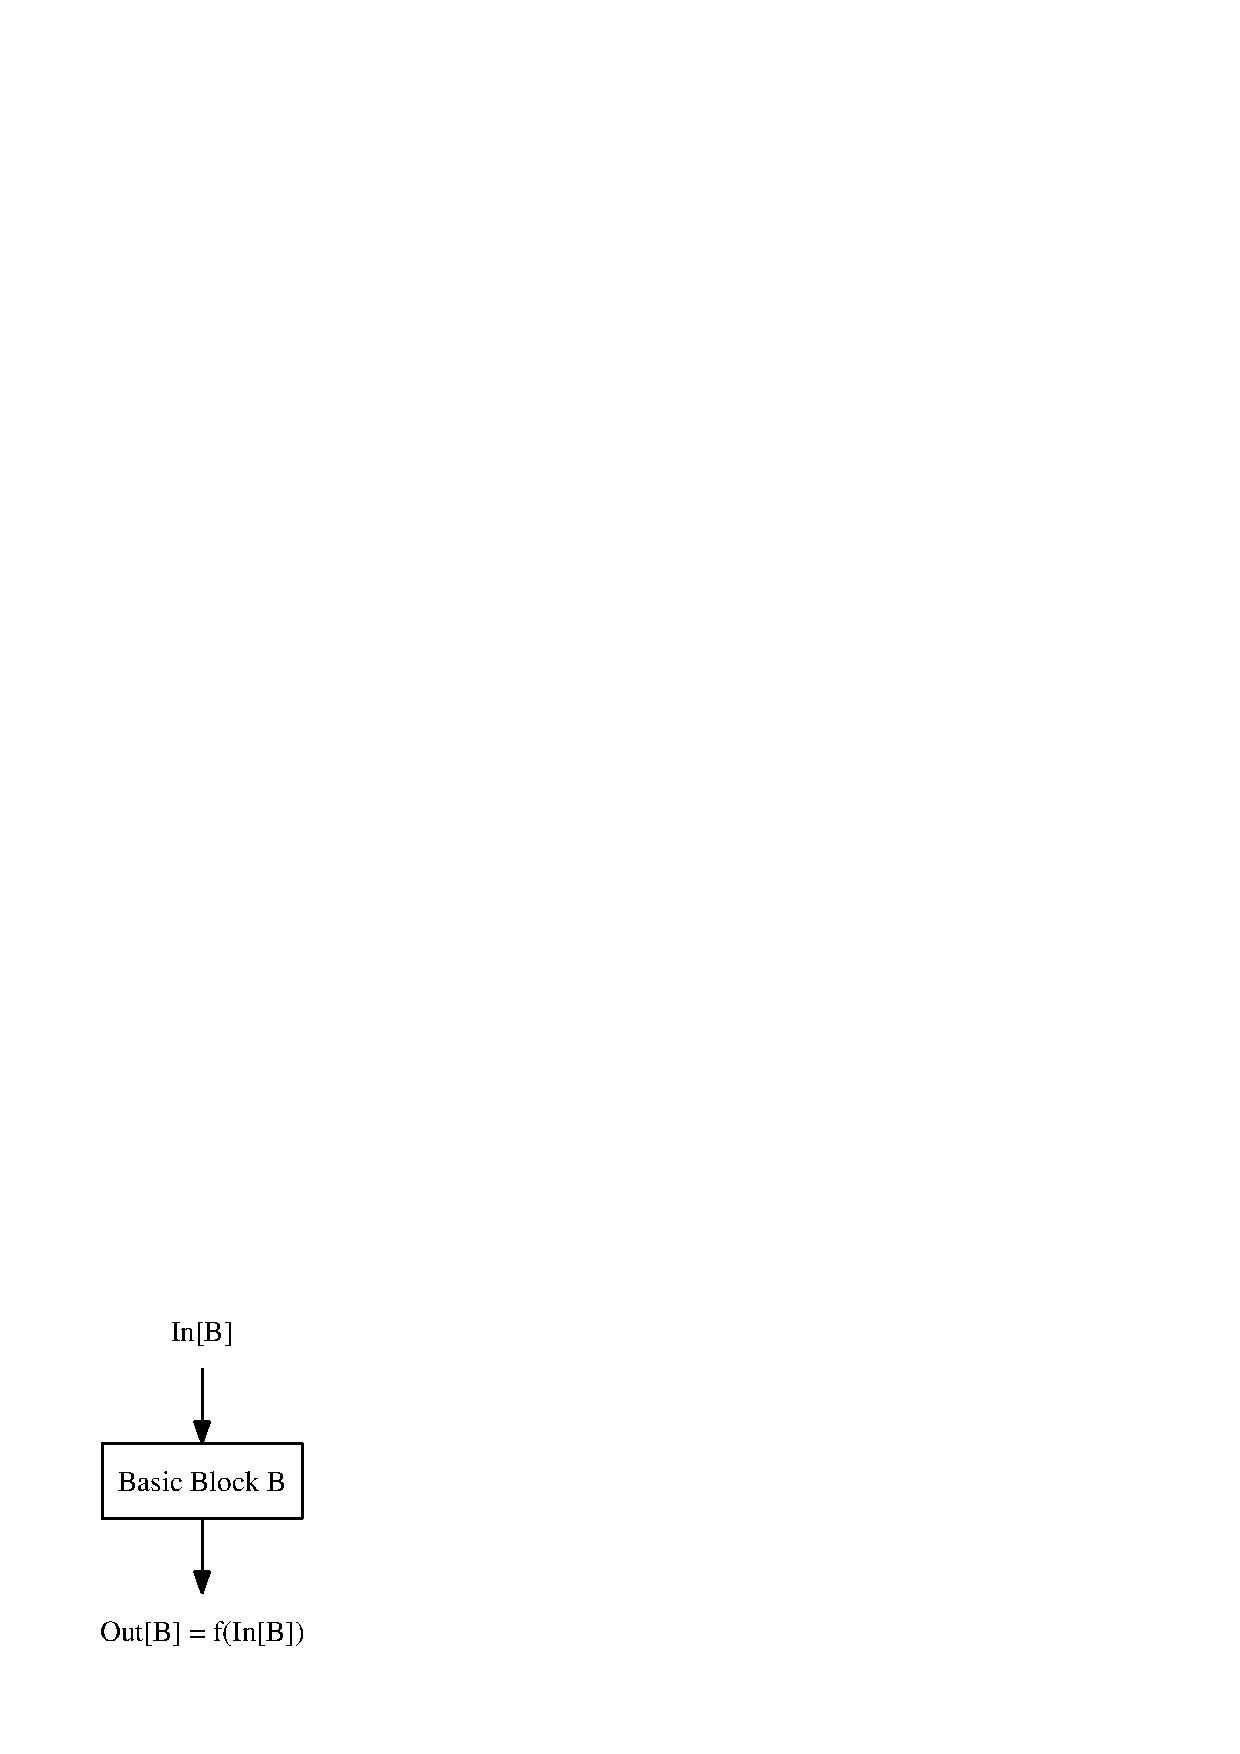
\includegraphics{grph2_text} 
    \label{labelname 1}
  \end{minipage}
  \begin{minipage}[b]{6 cm}
    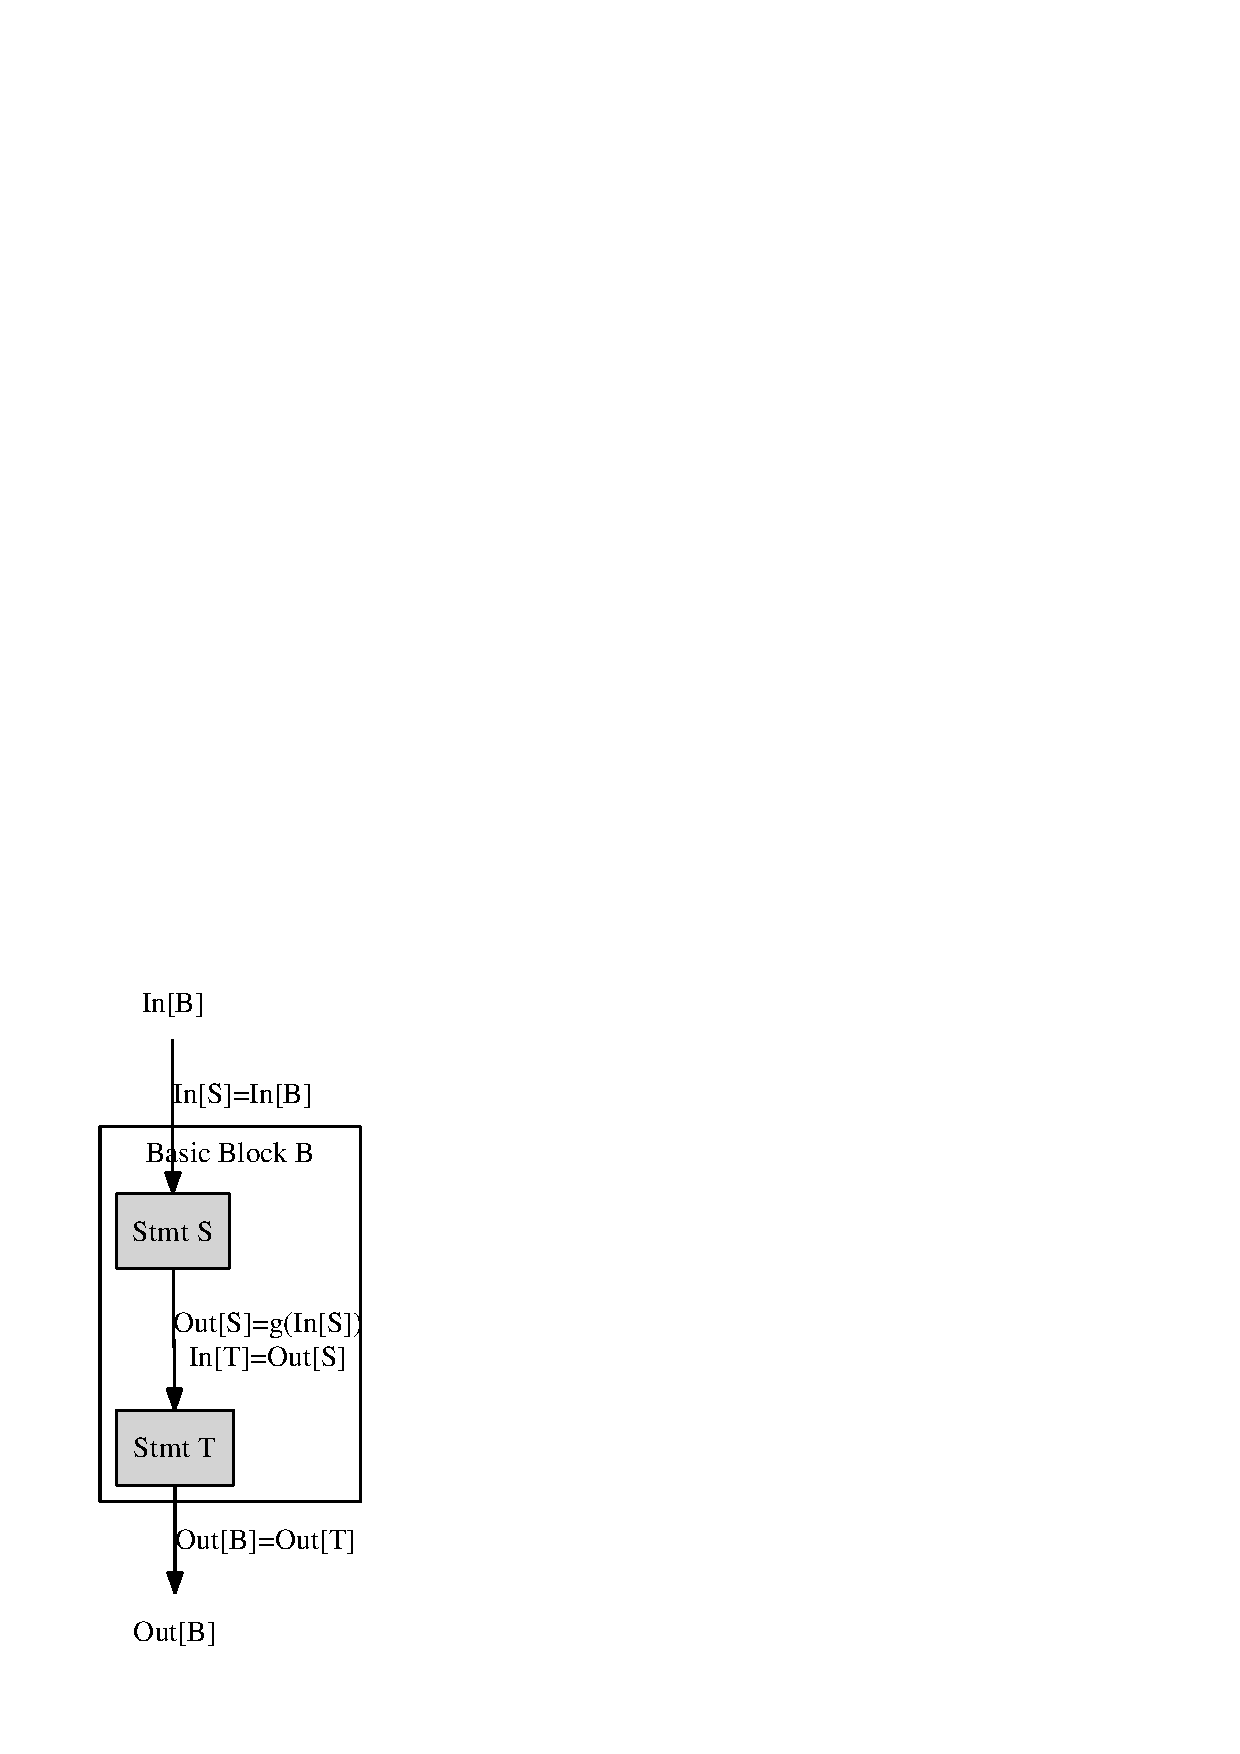
\includegraphics{grph3_text}  
%    \caption{caption 2}
    \label{labelname 2}
  \end{minipage}
  \caption{Transfer function for basic block}
   \label{fig:trans}
\end{figure}
%%%%%%%%%%%%%%%%%%%%%%%%%%%%%%%%%%%%
\begin{table}
\centering
\begin{tabular}{| l | c | c |}
\hline 
Statement & Gen set & Kill set \tn
\hline \hline
1. {\tt p = q} & {\tt \{<p,m> | <q,m>$\in$In[S]\}} & {\tt \{<p,l> | <p,l>$\in$In[S]\}} \tn
2. {\tt p = q\rtarrow next} & {\tt \{<p,m\rtarrow next> | <q,m>$\in$In[S]\}} & {\tt \{<p,l> | <p,l>$\in$In[S]\}} \tn
3. {\tt $\cdots$ = p\rtarrow data} & $\phi$ & $\phi$ \tn
4. {\tt p$\rightarrow$data = $\cdots$} & $\phi$ & $\phi$ \tn
5. {\tt fun(p, q)} & $\phi$ & $\phi$ \tn
\hline
\end{tabular}
\caption{\emph{Gen} and \emph{Kill} set for each statement} 
\label{fig:genKill}
%\hrule
\end{table}

The overall algorithm for state analysis is outlined in Figure~\ref{fig:AlgoStateAnal}. 
\ttf{Out[Entry]} is initialized to {\tt InitSet} to set the boundary condition. 
The \emph{while} loop in the algorithm iterates until it reaches the fixed-point. 
{\tt stateTrans} gives the algorithm for transfer function which works on each block. 
Though {\tt Gen} and {\tt Kill} informations are local to each statement they are 
computed in each iteration of the analysis, conflicting general data flow analysis algorithm. 
 
%%%%%%%%%%%%%%%%%%%%%%%%%%%%%%%%%%%%%%%%%%
\begin{figure}
%\hrule
\begin{framed}
{\tt
  \begin{program}{0}
  \FL fun stateAnalysis(CFG[f]:(N, E, Entry, Exit), k)  \{
  \UNL{0} Out[Entry] = InitSet; \COMMENT{Boundary condition}
  \UNL{0} \FOR each basic block B other than Entry
  \UNL{0} \COMMENT{Initialization for iterative algorithm}
  \UNL{1} Out[B] = $\phi$; 
  \UNL{0} \WHILE{(changes to any Out[ ] occur)} \{ \COMMENT{Iterate}
  \UNL{1} \FOR each basic block B other than Entry \{
  \UNL{2} In[B] = $\bigcup$(Out[P]), for all predecessors P of B;
  \UNL{2} Out[B] = stateTrans(B, In[B], k);
  \UNL{1} \}
  \UNL{0} \}
  \UNL{-1} \}
  \end{program}
}
\end{framed}
%\hrule
  \caption{Algorithm defining state analysis. \label{fig:AlgoStateAnal}}
%\hrule  
\end{figure}
%%%%%%%%%%%%%%%%%%%%%%%%%%%%%%%%%%%%%%%%%%%%%%%%%
\begin{figure}
%\hrule
\begin{framed}
{\tt
  \begin{program}{0}
  \FL fun stateTrans(Basic Block:BB, In set of BB:In[BB], k)  \{
  \UNL{0} TempState = In[BB];
  \UNL{0} \FOR each Stmt $S_i\in$ HeapStmt[BB] \{ \COMMENT{HeapStmt[BB] contains}
  \UNL{0} \COMMENT {heap intensive statements of BB}
  \UNL{1} In[$S_i$] = TempState;
  \UNL{1} Kill[$S_i$] = findStateDefVar(TempState, $S_i$);
  \UNL{1} Gen[$S_i$] = computeState(In[$S_i$], $S_i$);
%  \UNL{1} OldOut[$S_i$] = Out[$S_i$];
  \UNL{1} Out[$S_i$] = (In[$S_i$] - Kill[$S_i$]) $\cup$ Gen[$S_i$];
  \UNL{1} tempState = Out[$S_i$];
  \UNL{0} \}
  \UNL{0} return tempState;
  \UNL{-1} \}
  \end{program}
}
\end{framed}
%\hrule
  \caption{Algorithm for block level transfer function. \label{fig:AlgoGenState}}
%\hrule  
\end{figure}
%%%%%%%%%%%%%%%%%%%%%%%%%%%%%%%%%%%%
\begin{figure}
%\hrule
\begin{framed}
{\tt
  \begin{program}{0}
  \FL fun findStateDefVar(Set of States:TempState, Statement:$S_i$)  \{
  \UNL{0} Set of States : CurrState, LocalState = $\phi$;
%  \UNL{0} Set of variables used in Stmt : UseVarSet = $\phi$;
%  \UNL{0} UseVarSet = findUseVar(Stmt);\COMMENT{Detects variables used in Stmt}
  \UNL{0} \FOR each variable $V_i\in$ DefPtrSet \{
  \UNL{1} Find the state {\tt CurrState} of $V_i$ from {\tt TempState};
 \UNL{1} LocalState = LocalState $\cup$ CurrState;
  \UNL{0} \}
  \UNL{0} return LocalState;
  \UNL{-1} \}
  \end{program}
}
\end{framed}
%\hrule
  \caption{Computing \emph{Kill} set.\label{fig:AlgoFindStateDefVar}}
%\hrule  
\end{figure}
%%%%%%%%%%%%%%%%%%%%%%%%%%%%%%%%%%%%%%%%%%%%%%
\begin{figure}
%\hrule
\begin{framed}
{\tt
  \begin{program}{0}
  \FL fun computeState(In set of stmt:In[Stmt], Statement:Stmt)  \{
  \UNL{0} UseVarSet = findStateUseVar(In[Stmt], Stmt);
  \UNL{0} if Stmt $\equiv$ p = q 
  \UNL{1} Gen[Stmt] = \{ <p,$l_0$> | <q,$l_0$> $\in$ UseVarSet \} 
  \UNL{3} $\vee$ \{ <p,$l_0\rightarrow$sel> | <q,$l_0\rightarrow$sel> $\in$ UseVarSet \}
  \UNL{3} $\vee$ \{ <p,$l_0\rightarrow$sel$\rightarrow$*> | <q,$l_0\rightarrow$sel$\rightarrow$*> $\in$ UseVarSet \};
  \UNL{0} else if Stmt $\equiv$ p = q$\rightarrow$next
  \UNL{1} Gen[Stmt] = \{ <p,$l_0\rightarrow$next> | <q,$l_0$> $\in$ UseVarSet \} 
  \UNL{3} $\vee$ \{ <p,$l_0\rightarrow$sel$\rightarrow$*> | <q,$l_0\rightarrow$sel> $\in$ UseVarSet \};
  \UNL{0} else if Stmt $\equiv$ $\cdots$ = p$\rightarrow$data
  \UNL{1} Gen[Stmt] = In[Stmt];
  \UNL{0} else if Stmt $\equiv$ p$\rightarrow$data = $\cdots$
  \UNL{1} Gen[Stmt] = In[Stmt];
  \UNL{0} else if Stmt $\equiv$ f(p,q)
  \UNL{1} Gen[Stmt] = In[Stmt];
  \UNL{0} else Gen[Stmt] = $\phi$;
  \UNL{-1} \}
  \end{program}
}
\end{framed}
%\hrule
  \caption{Computing \emph{Gen} set. \label{fig:AlgoComputeState}}
%\hrule  
\end{figure}
%%%%%%%%%%%%%%%%%%%%%%%%%%%%%%%%%%%%%%%%%%
\begin{figure}
%\hrule
\begin{framed}
{\tt
  \begin{program}{0}
  \FL fun findStateUseVar(Set of States:TempState, Statement:$S_i$)  \{
  \UNL{0} Set of States : CurrState, LocalState = $\phi$;
%  \UNL{0} Set of variables used in Stmt : UseVarSet = $\phi$;
%  \UNL{0} UseVarSet = findUseVar(Stmt);\COMMENT{Detects variables used in Stmt}
  \UNL{0} \FOR each variable $V_i\in$ UsePtrSet \{
  \UNL{1} Find the state {\tt CurrState} of $V_i$ from {\tt TempState};
  \UNL{1} LocalState = LocalState $\cup$ CurrState;
  \UNL{0} \}
  \UNL{0} return LocalState;
  \UNL{-1} \}
  \end{program}
}
\end{framed}
%\hrule
  \caption{Computing states of used variables. \label{fig:AlgoFindStateUseVar}}
%\hrule  
\end{figure}
\begin{example}{\rm
We illustrate via an example the way our algorithm works. Let's consider the code fragment shown in Figure~\ref{ch:Intro}.2(b). 
Global variables and parameters of the code are initialized to {\tt InitSet} consisting of \ttf{\{<list, $l_0$>\}}. Table~\ref{fig:tableState} 
shows the set of states produced by each statement in the code and demonstrates how the analysis reaches fixed-point. 
Note that the length of access path is limited to 1. In this example \ttf{Out} set for each basic block in iteration number 2 is same as \ttf{Out} set produced by each block in iteration number 3. Hence in third iteration the algorithm reaches fixed-point.
}
\hfill\psframebox{}  \end{example}

\begin{table}
\centering
\begin{tabular}{| l | c | c |}
\hline 
Statement & Iteration 1 & Iteration 2 \tn
\hline \hline
S1: {\tt p = list} & {\tt In = \{<list,$l_0$>\}} & {\tt In = \{<list,$l_0$>\}} \tn %\cline{1-1}
& {\tt Gen = \{<p,$l_0$>\}} & {\tt Gen = \{<p,$l_0$>\}} \tn
& {\tt Kill = \{$\phi$\}} & {\tt Kill = \{$\phi$\}} \tn
& {\tt Out = \{<list,$l_0$>,<p,$l_0$>\}} & {\tt Out = \{<list,$l_0$>,<p,$l_0$>\}} \tn 
\hline
{\tt while() \{} & {\tt In = \{<list,$l_0$>,<p,$l_0$>\}} & {\tt In = \{<list,$l_0$>,<p,$l_0$>,} \tn %\cline{1-1}
& & {\tt <p,$l_0\rightarrow$next$\rightarrow${*}>,} \tn
& & {\tt <q,$l_0\rightarrow$next>,}\tn
& & {\tt <r,$l_0\rightarrow$next$\rightarrow${*}>\} = C}(say) \tn
%& & {\tt = C(say)} \tn
& {\tt Out = \{<list,$l_0$>,<p,$l_0$>\}} & {\tt Out = C} \tn
\hline
S2: {\tt q = p$\rightarrow$next} & {\tt In = \{<list,$l_0$>,<p,$l_0$>\}} & {\tt In = C} \tn %\cline{1-1}
& {\tt Gen = \{<q,$l_0\rightarrow$next>\}} & {\tt Gen = \{<q,$l_0\rightarrow$next>,} \tn
& & {\tt <q,$l_0\rightarrow$next$\rightarrow${*}>\}} \tn
& {\tt Kill = $\phi$} & {\tt Kill = \{<q,$l_0\rightarrow$next>\}} \tn
& {\tt Out = \{<list,$l_0$>,<p,$l_0$>,} & {\tt Out = \{C,<q,$l_0\rightarrow$next$\rightarrow${*}\}} \tn
& {\tt <q,$l_0\rightarrow$next>\} = A}(say)&  {\tt = D}(say) \tn
%& {\tt = A(say)}& {\tt = D(say)} \tn
\hline
S3: {\tt temp = q$\rightarrow$num} & {\tt In = A} & {\tt In = D} \tn
& {\tt Out = A} & {\tt Out = D} \tn
\hline
S4: {\tt r = q$\rightarrow$next} & {\tt In = A} & {\tt In = D} \tn
& {\tt Gen = \{<r,$l_0\rightarrow$next$\rightarrow${*}>\}} & {\tt Gen = \{<r,$l_0\rightarrow$next$\rightarrow${*}>\}} \tn
& {\tt Kill = $\phi$} & {\tt Kill = \{<r,$l_0\rightarrow$next$\rightarrow${*}>\}} \tn
& {\tt Out = \{A,<r,$l_0\rightarrow$next$\rightarrow${*}>\}} & {\tt Out = D} \tn
%& {\tt <r,$l_0\rightarrow$next$\rightarrow${*}>\}} & \tn
& {\tt = B}(say) & \tn
\hline
S5: {\tt r$\rightarrow$num = temp} & {\tt In = B} & {\tt In = D} \tn
& {\tt Out = B} & {\tt Out = D} \tn
\hline
S6: {\tt p = r} & {\tt In = B} & {\tt In = D} \tn
& {\tt Gen = \{<p,$l_0\rightarrow$next$\rightarrow${*}>\}} & {\tt Gen = \{<p,$l_0\rightarrow$next$\rightarrow${*}>\}} \tn
& {\tt Kill = \{<p,$l_0$>\}} &{\tt Kill = \{<p,$l_0$>,} \tn
& & {\tt <p,$l_0\rightarrow$next$\rightarrow${*}>\}} \tn
& {\tt Out = \{<list,$l_0$>,} & {\tt Out = \{<list,$l_0$>,} \tn
& {\tt <p,$l_0\rightarrow$next$\rightarrow${*}>,} & {\tt <p,$l_0\rightarrow$next$\rightarrow${*}>,} \tn
& {\tt <q,$l_0\rightarrow$next>,} & {\tt <q,$l_0\rightarrow$next>,} \tn
& {\tt <r,$l_0\rightarrow$next$\rightarrow${*}>\}} & {\tt <q,$l_0\rightarrow$next$\rightarrow${*}>,} \tn
& & {\tt <r,$l_0\rightarrow$next$\rightarrow${*}>\}} \tn
\hline
\end{tabular}
\caption{Set of states for each statement of an example code} 
\label{fig:tableState}
%\hrule
\end{table}

%%%%%%%%%%%%%%%%%%%%%%%%%%%%%%%%%%%%%%%%%%%%%%%%%%%%s
\begin{figure}
%\hrule
\begin{framed}
{\tt
  \begin{program}{0}
  \FL fun computeReadWrite(Set of States:HeapStates)  \{
  \UNL{0} Set of States : CurrState, LocalState = $\phi$;
  \UNL{0} \FOR each stmt $S_i$ \{
  \UNL{1} \IF ($S_i$ $\equiv$ $\cdots$ = p$\rightarrow$num) \{ \COMMENT{statement reading heap}
  \UNL{2} ReadSet = findStateUseVar (HeapStates[$S_i$], $S_i$);
  \UNL{2} WriteSet = $\phi$;
  \UNL{1} \}
  \UNL{1} \IF else ($S_i$ $\equiv$ p$\rightarrow$num = $\cdots$) \{ \COMMENT{statement writing into heap}
  \UNL{2} ReadSet = $\phi$;
  \UNL{2} WriteSet = findStateUseVar (HeapStates[$S_i$], $S_i$);
  \UNL{1} \}
  \UNL{1} \IF else ($S_i$ $\equiv$ f(p,q)) \{ \COMMENT{function call statement}
  \UNL{2} ReadSet = findStateUseVar (HeapStates[$S_i$], $S_i$);
  \UNL{2} WriteSet = findStateUseVar (HeapStates[$S_i$], $S_i$);
  \UNL{1} \}
  \UNL{1} else \{
  \UNL{2} ReadSet = $\phi$;
  \UNL{2} WriteSet = $\phi$;
  \UNL{1} \}
  \UNL{0} \}
  \UNL{-1} \}
  \end{program}
}
\end{framed}
%\hrule
  \caption{computing Read and Write sets. \label{fig:AlgoReadWrite}}
%\hrule  
\end{figure}
%%%%%%%%%%%%%%%%%%%%%%%%%%%%%%%%%%%%%%%%%%%%%%%%%%%%%%
\subsection{Read/Write State Computation}
For each statement we intend to compute two sets of heap access 
paths: (a)\emph{Read set}: the set of paths which are accessed 
to read a heap location and (b)\emph{Write set}: the set of paths 
which are accessed to write to a heap location. These sets are 
obtained from the set of states, generated by the state analysis, in a single 
pass over the function. The read and write sets are used 
later to identify dependences. 

Function {\tt computeReadWrite} 
referred in Figure~\ref{fig:AlgoReadWrite} computes such sets in a 
single symbolic execution of the function. 
Function {\tt findStateUseVar} is used to generate {\tt Read} 
and {\tt Write} sets for statements reading/writing heap. Function calls are handled by
conservative read/write sets that over approximate the
heap locations that could potentially be read or written
inside the called function. Read and write sets for other statements are set to $\phi$. 

 \begin{figure}[t]
  \begin{center}
  
    \scalebox{.8}{\begin{tabular}{ c | c }
%    \hline
      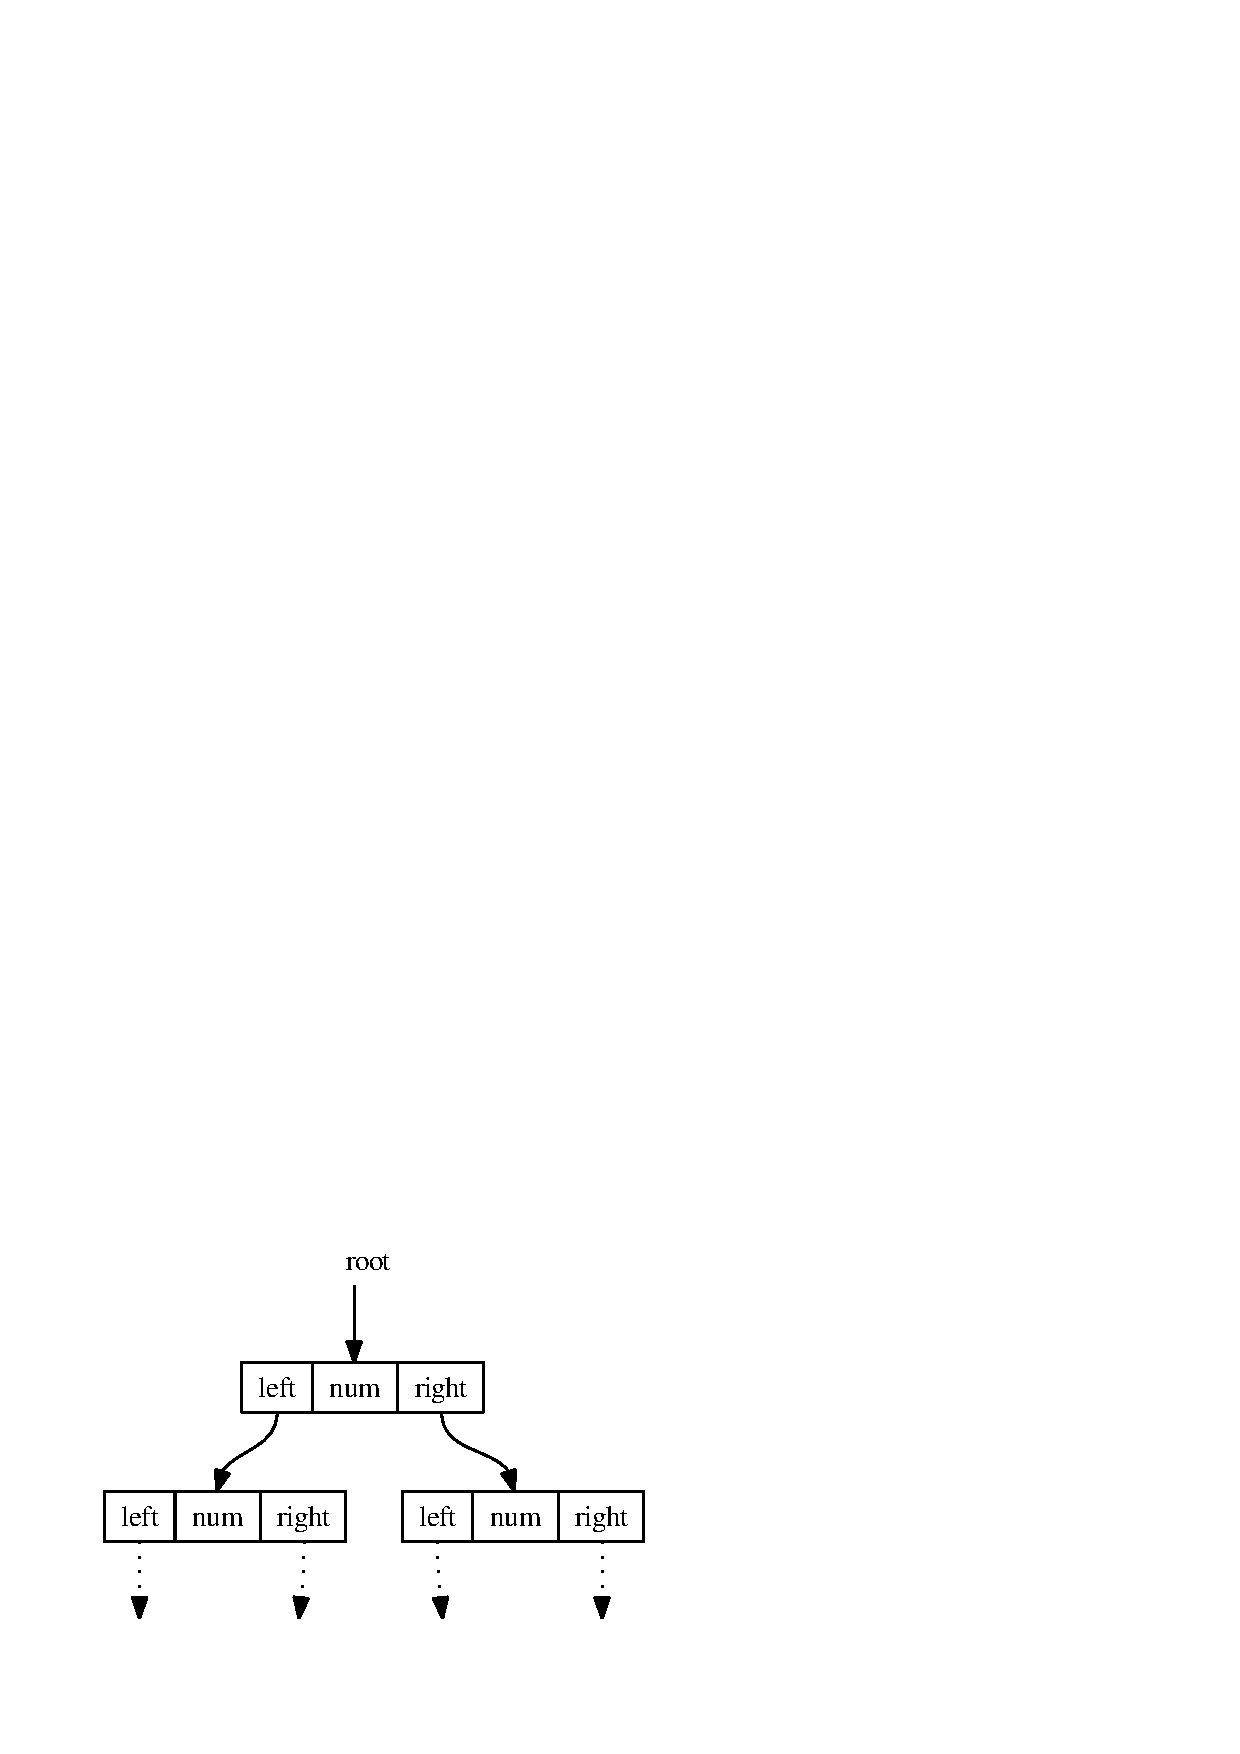
\includegraphics[scale=0.75]{tree_grph} %\cline{1-1}
      &
      {\tt
\begin{program}{10}
  \FL\ \ldots
  \NL{0} p = tree;
  \UNL{0} \WHILE (p$\rightarrow$left != NULL) \{
  \NL{1}     newFunc (p);
%  \NL{1}     temp = q$\rightarrow$num;
  \NL{1}     p = p$\rightarrow$left;
%  \NL{1}     r$\rightarrow$num = temp;
%  \NL{1}     myFunc (q, r);
%  \NL{1}     p = r;
  \UNL{0} \}
  \UNL{0} \ldots \\
 \\
 \\
 \\
 \\
  %
\end{program}
}
 \\
      (a) Tree data structure. & 
      (b) Code fragment traversing the data structure. \\
%      \hline
    \end{tabular}}
  \end{center}
  \hrule
  \caption{\label{fig:func} Program with function call.}
\end{figure}
%
\begin{example}{\rm Consider the code fragment shown in Figure~\ref{fig:func}(b) which traverses 
the Tree data structure shown in Figure~\ref{fig:func}(a). 
Our analysis conservatively approximates read and write sets for statement \ttf{S12} which is a function call statement. 
The analysis generates the read and write sets as \ttf{\{<p, $l_0$>, 
<p, $l_0$\rtarrow{*}>\}} which is the worst case approximations of such sets. 
}
\hfill\psframebox{}  \end{example}

Our approach is conservative in the sense that the read set
and write set we compute for a statement are over
approximations of the actual locations that are read or
written by the statement. Therefore it is possible that our
analysis reports two statement to be dependent when they are
not really dependent on each other. However, this can inhibit
some parallelizing optimization but can not result in an
incorrect parallelization. 
\begin{table}
\centering
\begin{tabular}{| l | c | c |}
\hline 
Statement & Read set & Write set \tn
\hline
S1: {\tt p=list} & {\tt $\phi$} & {\tt $\phi$}\tn
S2: {\tt q=p$\rightarrow$next} & {\tt $\phi$} & {\tt $\phi$} \tn
S3: {\tt temp=q$\rightarrow$num} & {\tt \{<q,$l_0\rightarrow$next>,} & {\tt $\phi$} \tn
& {\tt <q,$l_0\rightarrow$next$\rightarrow${*}>\}} & \tn
S4: {\tt r=q$\rightarrow$next} & {\tt $\phi$} & {\tt $\phi$} \tn
S5: {\tt r$\rightarrow$num=temp} & {\tt $\phi$} & {\tt \{<r,$l_0\rightarrow$next$\rightarrow${*}>\}}\tn
%S6: {\tt myFunc(p,q)} & {\tt \{<p,$l_0\rightarrow$next>,} & {\tt \{<p,$l_0\rightarrow$next>,} \tn
%& {\tt <p,$l_0\rightarrow$next$\rightarrow${*}>,} & {\tt <p,$l_0\rightarrow$next$\rightarrow${*}>} \tn
%& {\tt <q,$l_0\rightarrow$next>,} & {\tt <q,$l_0\rightarrow$next>,} \tn
%& {\tt <q,$l_0\rightarrow$next$\rightarrow${*}>\}} & {\tt <q,$l_0\rightarrow$next$\rightarrow${*}>\}} \tn
S6: {\tt p=r} & {\tt $\phi$} & {\tt $\phi$} \tn
\hline
\end{tabular}
\caption{Read and write sets accessed by each statement} 
\label{fig:tableReadWrite}
%\hrule
\end{table}
\subsection{Dependence Detection}
Our approach identify memory locations in terms of 
access paths as mentioned earlier. Multiple access 
paths can exist at a time leading to same location. 
Hence we need some method to detect whether two paths 
access same location or not. Our analysis needs to know 
if any two access paths potentially share a common heap object. 
Shape analysis as referred in~\cite{sandeep} produces an 
interface \ttf{isInterfering(p, $\alpha$, q, $\beta$)} 
to detect such interference. For heap pointers \ttf{p}, 
\ttf{q} and field sequences $\alpha, \beta, \alpha', \beta'$, 
this function returns true if the
paths {\tt p.$\alpha'$} and {\tt q.$\beta'$} interfere
(potentially reach the same heap node at run-time), and
$\alpha$ and $\beta$ are prefixes of $\alpha'$ and $\beta'$
respectively.

Read and write sets thus generated are tested to detect 
various dependences (flow, anti or output). Let \ttf{S} and \ttf{T} 
be statements in the program such that there exists an execution 
path from \ttf{S} to \ttf{T}. Then the dependence of \ttf{T} on 
\ttf{S} can be defined as follows:

\newcommand{\flowdep}{\mbox{flow-dep}}
\newcommand{\antidep}{\mbox{anti-dep}}
\newcommand{\outputdep}{\mbox{output-dep}}
\newcommand{\rs}[1]{\mbox{read}(#1)}
\newcommand{\ws}[1]{\mbox{write}(#1)}
\newcommand{\rst}[2]{\mbox{read}(#1, #2)}
\newcommand{\wst}[2]{\mbox{write}(#1, #2)}
\newcommand{\set}{\mbox{set}}
\noindent

$\begin{array}{rcl}
\interf{\set_1}{\set_2} &\equiv& \isInterfering(p, \alpha, q,
\beta) \; \mbox{where } 
p.\alpha \in \set_1   \wedge  q.\beta \in \set_2 \\ 
\flowdep(S, T) &\equiv& \interf{\ws{S}}{\rs{T}} \\ 
\antidep(S, T) &\equiv& \interf{\rs{S}}{\ws{T}} \\
\outputdep(S, T) &\equiv& \interf{\ws{S}}{\ws{T}}
\end{array}$ \\
\noindent where \isInterfering\ is the function provided by
shape analysis.

\begin{example} {\label{ex:dep}\rm
Table~\ref{fig:tableReadWrite} shows the read and write sets for each statement in
the example code of Figure~\ref{ch:Intro}.2(b). From the table,
we can infer all the dependences of which few are listed here:
\begin{enumerate}
\item loop independent anti-dependence  from statement {S3} to
statement {S5}
\item loop carried flow-dependence  from statement {S5} to
statement {S3}
\item loop independent output-dependence from statement {S5} 
to statement {S6}
\item loop carried anti-dependence from statement {S6} to statement {S5}
\end{enumerate}  
Due to presence of loop carried dependences different iterations of the loop can not be executed in parallel. Next we explain how we can further refine our dependence
analysis to filter out some spurious dependences.
}
\hfill\psframebox{}  \end{example}


\chapter{Loop Sensitive Dependence Analysis}
\label{ch:loopdep}
This chapter focuses on detecting the presence of dependences on loops which 
traverse recursive heap data structure. Two statements \ttf{S} and \ttf{T} may induce (a) \ttf{Loop Independent Dependence} (LID), where statements \ttf{S} and \ttf{T}
access same memory location in a single iteration of the loop, (b) \ttf{Loop Carried Dependence} (LCD), if the 
memory location accessed by statement \ttf{S} in a given iteration, is accessed 
by statement \ttf{T} in other iteration. In either case at least one of the accesses must be write access. 

Our approach for dependence analysis, as explained earlier, does not work well 
for loops. This is because it combines the paths accessed in different iterations 
of a loop.  To get better result in
presence of loops we need to keep the accesses made by
different iterations of a loop separate. To do so, we have
devised another novel approach, which works as follows: Given
a loop, we first identify the navigators for the loop,
then by a single symbolic traversal over the loop, we compute
the read and write accesses made by each statement in terms
of the values of the navigators. The read and write sets thus
obtained are generalized to represent arbitrary iteration of
the loop, using the iteration number as a parameter. These generalized 
sets, in terms of equations, are tested by \emph{GCD} or \emph{Lamport} test 
to find out any integer solution of those equations. Presence of loop dependences
indicates that the iterations are not independent, hence 
can not be executed in parallel. The top level algorithm of loop analysis is 
outlined in Figure~\ref{fig:algoLoopAnalyse}.

We assume that the loop under analysis is heap intensive i,e., 
reads/writes heap and the execution of the loop does not stop 
prematurely using irregular control flow constructs 
such as \emph{return}, \emph{continue}, \emph{break} 
statements or function calls like \emph{exit}, \emph{abort}. 
Hence testing loop condition is the only way to exit 
control from the loop. 

The rest of the 
chapter is organised as follows: Section~\ref{sec:nav} gives a
brief description of finding navigator of the loop. Section~\ref{sec:DepDetect} 
explains about how to compute read and wriets sets of access 
paths and how our approach identifies both loop independent and
loop carried dependences.
\begin{figure}
%\hrule
\begin{framed}
{\tt
  \begin{program}{0}
  \FL fun loopAnalyse(Loop)  \{
%  \UNL{0} GoodLoop = detectGoodLoop(f);
  \UNL{0} <NavigatorVar, NavigatorExpr>  = identifyNavigator(Loop);%\COMMENT{returns both navigator variable and navigator expr}
  \UNL{0} ReadWriteSet = generateReadWrite(NavigatorVar);
  \UNL{0} identifyDep(ReadWriteSet);
  \UNL{-1} \}
  \end{program}
}
\end{framed}
%\hrule
  \caption{Dep. detection for loop. \label{fig:algoLoopAnalyse}}
%\hrule  
\end{figure}
%%%%%%%%%%%%%%%%%%%%%%%%%%%%%%%%%%%%%%%%%%%%%%%%%%%%%%%%%%
\section{Identifying Navigator}
\label{sec:nav}
Dependence analysis for loops relies on the computation of read and write sets, 
in terms of access path, for each statement in a single symbolic iteration of the loop. 
Access paths are computed with respect to \emph{navigator} as mentioned 
in~\cite{ghiya98detecting}. A navigator consists of (a)\emph{navigator variable} \ttf{NavigatorVar}, pointer variable 
used to traverse the loop and (b)\emph{navigator expression} \ttf{NavigatorExpr}, ordered set of pointer field references. 
Navigator variable in association with the navigator expression, iterates the loop traversing the data structure.

Navigator variable is closely related to the variable {\tt TestVar} used to test the stopping criteria
for the loop in the program. The algorithm generates the definition chain \ttf{DefChain} of 
{\tt TestVar} using statements inside the loop. If the definition chain of \ttf{TestVar} encounters a 
loop resident statement twice, recurrence is reported. Otherwise the creation of definition chain returns 
null if it fails to find a loop resident statement for \ttf{DefChain}. 
Hence {\tt DefChain}, thus generated for the 
later case returns an access path consisting of a pointer variable followed by an ordered sequence of pointer field references. 
The base pointer variable obtained from the access path is potential candidate to be navigator variable and the  
sequence of field references results in navigator expression. The details for identifying navigator can be found 
in~\cite{ghiya98detecting}. 

\begin{example}{\rm
Consider the code shown in Figure~\ref{ch:Intro}.2(b). We identify 
\ttf{p} as loop condition test variable. Definition chain for \ttf{p} comes from the sequence of following loop-resident statements, 
{\tt S7: p = r}, {\tt S4: r = q\rtarrow next}, {\tt S2: q = p\rtarrow next} and {\tt S7: p = r}. Note that statement {\tt S7} is
encountered twice, leading to recurrence. Hence the statements {\tt S7}, {\tt S4}, {\tt S2} are added to {\tt DefChain} which returns 
access path as {\tt p\rtarrow next\rtarrow next}. Hence the resulting navigator consists of navigator variable {\tt p} and navigator expression 
{\tt next\rtarrow next}
}
\hfill\psframebox{}  \end{example}
%%%%%%%%%%%%%%%%%%%%%%%%%%%%%%%%%%%%%%%%%%%%%%%%%%%%%%%%%%%%%%%%%%%%%%%%%%%%%%%%%%%%
\section{Computing Read/Write Sets}
As mentioned earlier, our analysis computes read and 
write sets for each statement residing in the loop in 
a single symbolic execution of the loop. Read and write sets 
consist of paths that access heap locations for reading or writing. Unlike previous analysis, 
full length access paths are used by loop dependence analysis. For each 
loop-residing statement full length access paths, referred as \ttf{AccPath}, 
are computed in terms of navigator variable. Access paths \ttf{AccPath} 
are computed from definition chains, that are evaluated by recursively 
traversing all the reaching definitions of the pointer variable 
used by the statement until 
the navigator variable is encountered. 

\begin{figure}
%\hrule
\begin{framed}
{\tt
  \begin{program}{0}
  \FL fun generateReadWrite(NavigatorVar)  \{
%  \UNL{0} CFG[f] = (N, E, Entry, Exit); \COMMENT {Control flow graph of function f}
 % \UNL{0} InitSet = initialize(); \COMMENT{Initialize all parameters and
%  globals}
  \UNL{0} for each statement $S_i$ in Loop \{
  \UNL{1} UseVar = UseVarSet[$S_i$];
  \UNL{1} DefChain[$S_i$] = findDefChain(UseVar, NavigatorVar);
  \UNL{1} AccPath[$S_i$] = findAccPath(DefChain[$S_i$]);
  \UNL{1} if (Tag[$S_i$] == ReadStmt) \{
  \UNL{2} ReadSet[$S_i$] = AccPath[$S_i$];
  \UNL{2} WriteSet[$S_i$] = $\phi$;
  \UNL{1} \}
   \UNL{1} else if (Tag[$S_i$] == WriteStmt) \{
  \UNL{2} WriteSet[$S_i$] = AccPath[$S_i$];
  \UNL{2} ReadSet[$S_i$] = $\phi$;
  \UNL{1} \}
   \UNL{1} else \{
  \UNL{2} ReadSet[$S_i$] = $\phi$;
  \UNL{2} WriteSet[$S_i$] = $\phi$;
  \UNL{1} \}
  \UNL{0} \}
  \UNL{-1} \}
  \end{program}
}
\end{framed}
%\hrule
  \caption{Generating Read and Write sets. \label{fig:algoReadWrite}}
%\hrule  
\end{figure}

These access paths, thus constructed, return 
read/write sets based on statements reading or writing heap data. 
Function \ttf{generateReadWrite} showed in Figure~\ref{fig:algoReadWrite} 
computes such sets of access paths with respect to navigator variable \ttf{NavigaotrVar}.
Definition chain, \ttf{DefChain}, produced by function \ttf{findDefChain}, 
is processed by function \ttf{findAccPath} to compute access path. 
\ttf{ReadSet}/\ttf{WriteSet} sets, for each statement, are then computed from \ttf{AccPath}. 
The access paths, thus obtained, 
are generalized by arbitrary iteration of the loop, using iteration number as parameter, for further processing. 
\begin{example}{\rm
Let us again consider the example given in Figure~\ref{ch:Intro}.2(b). 
Navigator variable and navigator expression for the loop are \ttf{p} and \ttf{next\rtarrow{next}} 
respectively. Table~\ref{fig:tableLoopReadWrite} shows the read and write sets of full access paths constructed for each loop residing statement. Note that, 
the access paths are not abstracted and are constructed in terms of \ttf{p}. 
}
\hfill\psframebox{}  \end{example}
\begin{table}
\centering
\begin{tabular}{| l | c | c |}
\hline 
Statement & Read Set & Write Set \tn
\hline \hline
{\tt S2} & $\phi$ & $\phi$ \tn
{\tt S3} & \ttf{p\rtarrow{next}} & $\phi$ \tn
{\tt S4} & $\phi$ & $\phi$ \tn
{\tt S5} & $\phi$ & \ttf{p\rtarrow{next}\rtarrow{next}} \tn
{\tt S6} & $\phi$ & $\phi$ \tn
\hline
\end{tabular}
\caption{Read and write sets for each loop residing statement} 
\label{fig:tableLoopReadWrite}
%\hrule
\end{table}
%%%%%%%%%%%%%%%%%%%%%%%%%%%%%%%%%%%%%%%%%%%%%%%%%%%%%%%%%%%%%%%%%%%%%%%%%%%%%%%%%
%%%%%%%%%%%%%%%%%%%%%%%%%%%%%%%%%%%%%%%%%%%%%%%%%%%%%%%%%%%%%%%%%%%%%%%%%%%%%%%%%%%
\section{Loop Dependence Detection}
\label{sec:DepDetect}
Let \ttf{S} and \ttf{T} be two statements inside a loop. Further, 
let \ttf{write(S,i)} denote the set of access paths written by statement 
\ttf{S} in the iteration number \ttf{i}, and let \ttf{read(T,j)} 
denote the set of access paths read by statement \ttf{T} in the iteration
number \ttf{j}. Predicate \ttf{sharing}($\ttf{Set}_\ttf{1}$, $\ttf{Set}_\ttf{2}$) returns 
true if two access paths $\ttf{AccPath}_\ttf{1}\in\ttf{Set}_\ttf{1}$ and $\ttf{AccPath}_\ttf{2}\in\ttf{Set}_\ttf{2}$ 
share a common heap node. Then
\begin{itemize}
\item \ttf{T} is loop independent flow dependent on \ttf{S} if there is an 
execution path from \ttf{S} to \ttf{T} that does not cross the loop boundary and there exist \ttf{i} 
within loop bounds such that \ttf{sharing(write(S,i), read(T,i))} is true.
\item \ttf{T} is loop carried flow dependent on \ttf{S} if there exist 
\ttf{i} and \ttf{j} within loop bounds such that \ttf{j}>\ttf{i}, and \ttf{sharing(write(S,i), read(T,j))} is true.
\end{itemize}
Note that, in case loop bounds can not be computed at compile time,
we can assume them to be (-$\infty$,$\infty$). We can similarly define 
loop independent and loop carried anti-dependence and output-dependence.
Read and write sets of access paths, thus obtained for 
each statement inside a loop are tested for both loop independent 
and loop carried dependences.
%%%%%%%%%%%%%%%%%%%%%%%%%%%%%%%%%%%%%%%%%%%%%%%%%%%%%%%%%%%%%%%%%%%%%%%%%%%%%%%%%%%%%%
%%%%%%%%%%%%%%%%%%%%%%%%%%%%%%%%%%%%%%%%%%%%%%%%%%%%%%%%%%%%%%%%%%%%%%%%%%%%%%%%%%%%%% 
\subsection{Identifying Loop Independent Dependence}
Loop independent dependences can be detected for 
any two statements by checking for any sharing of node by their 
respective read/write sets. Sharing of a node, in this level, occurs due to 
the shape of the underlying data structure. Shape analysis gives the 
probable shape attribute of the navigator variable traversing dynamic data structure. Based 
on the shape we can figure out whether 
there exists any dependence due to sharing within the underlying data structure. 
\begin{description}
\item[Observation 1:]If the shape attribute of navigator variable is Tree, then there 
exist no sharing of nodes by different access paths rooted at the navigator variable. Two access paths can only visit 
a common node if the paths are equivalent. Let \ttf{lp} be the navigator variable. Hence \ttf{lp\rtarrow{f}} and \ttf{lp\rtarrow{f}} 
are equivalent paths leading to a common node, whereas \ttf{lp\rtarrow{f}} and \ttf{lp\rtarrow{g}} lead to different nodes.

\item[Observation 2:] If the shape attribute is DAG, the navigator expression will lead navigator 
variable to a distinct node in each iteration of the loop. If an access path is a proper subpath 
of another access path then they surely visit distinct nodes. However, paths being either equivalent or distinct, having different 
pointer field references may access a common node. For example, \ttf{lp\rtarrow{f}} is a proper subpath of 
\ttf{lp\rtarrow{f}\rtarrow{g}} whereas, \ttf{lp\rtarrow{f}} and 
\ttf{lp\rtarrow{g}} are not. Hence in the former case they do not share a common node, whereas  
in later case they might result in sharing of node.

\item[Observation 3:] If shape attribute of navigator variable is Cycle, we make conservative decision such that the loop can 
not be executed in parallel.
\end{description}
To detect various types of LIDs, read and write sets of different statements are tested 
accordingly for detecting sharing of node. Let two statements \ttf{S} and \ttf{T} access paths 
\ttf{PathS} and \ttf{PathT} respectively and \ttf{read(S) = \{PathS\}} and \ttf{write(T) = \{PathT\}}. 
Hence there is loop independent flow dependence from \ttf{S} to \ttf{T} if \ttf{sharing(PathS, PathT)} returns true.
We check for the shape of the underlying data structure 
and test the paths as follows:
\begin{enumerate}
\item If the paths \ttf{PathS} and \ttf{PathT} are equivalent and the data structure is either Tree or DAG, 
the paths will access same node. Hence,
\[ \ttf{sharing (PathS, PathT)} = True\] for both Tree and DAG structure.
\item If \ttf{PathS} is subpath of \ttf{PathT} then these paths do not lead to any common node for both Tree 
and DAG data structure. Hence, 
\[ \ttf{sharing (PathS, PathT)} = False\] for both Tree and DAG structure.
\item If \ttf{PathS} and \ttf{PathT} are not equivalent and one is not subpath of other, then these two paths share a common node only if 
shape of the underlying structure is DAG. For Tree structure they lead to disjoint nodes. 
\[ \ttf{sharing (PathS, PathT)} = False\] if shape attribute is TREE.
\[ \ttf{sharing (PathS, PathT)} = True\] if shape attribute is DAG.
\end{enumerate}
\begin{example}{\rm
Consider the loop shown in Figure~\ref{ch:Intro}.2(b) and the corresponding 
read and write sets for each statement in Table~\ref{fig:tableLoopReadWrite}. Read set of statement
\ttf{S3} and write set of statement \ttf{S5} are checked for sharing of any  node. As the shape attribute 
of the navigator variable \ttf{p} is Tree, and the paths \ttf{p\rtarrow{next}} and 
\ttf{p\rtarrow{next}\rtarrow{next}} are not equivalent the following will result.
\[\ttf{sharing(p\rightarrow{next}, p\rightarrow{next}\rightarrow{next})} = False\]
Hence no loop independent dependence is detected. 
}
\hfill\psframebox{}  \end{example}
%%%%%%%%%%%%%%%%%%%%%%%%%%%%%%%%%%%%%%%%%%%%%%%%%%%%%%%%%%%%%%%%%%%%%%%%%%%%%%%%%%%%
%%%%%%%%%%%%%%%%%%%%%%%%%%%%%%%%%%%%%%%%%%%%%%%%%%%%%%%%%%%%%%%%%%%%%%%%%%%%%%%%%%%%
\subsection{Identifying Loop Carried Dependence}
Loop carried dependence is incurred in the loop when two statements from different 
iterations access same memory location. LCDs can be introduced 
when the statements in a single iteration of loop access both current node and neighbour heap nodes.  
Current node means the node which is being currently accessed by the navigator 
variable, whereas, neighbour nodes mean nodes other than the one being currently 
accessed. 
\begin{example}{\rm
Let the shape attribute of the navigator variable \ttf{lp} be Tree and 
a loop is traversing a list using navigator variable \ttf{lp} and navigator expression \ttf{next}. 
Statement \ttf{lp\rtarrow{num}++} will not incur any loop carried dependence as 
the location pointed to by \ttf{lp} can't be accessed in consecutive iterations. 
However, statement like \ttf{lp\rtarrow{num} = lp\rtarrow{next}\rtarrow{num}} 
will still introduce an LCD because both current and neighbour nodes are accessed 
in the same iteration and neighbour node is visited using pointer field \ttf{next} 
which is also a navigator expression. 
}
\hfill\psframebox{}  \end{example}
As mentioned earlier, LCDs are only introduced by different iterations of loop, provided there is 
no sharing of nodes hidden in the data structure. However, DAG has sharing within the 
structure, it can be traversed by a loop in a manner such that shared nodes 
are not accessed by loop and access pattern of the structure is Tree. Hence, loops having this type 
of access pattern can also be tested for loop carried dependencies. 

The read-write sets computed by each loop resident statements are generalized 
for arbitrary iteration number, resulting in a set of equations. Generalization is done 
using random times of navigator expression, that is used by the navigator variable to traverse 
over the underlying data structure. These equations are then tested 
by \ttf{GCD}~\cite{Kennedy01Optimizing} or \ttf{Lamport}~\cite{Lamport1974parallel} test, as explained before. If the equations have any integer solution, 
dependence is reported. 
Here we demonstrate two examples to show the novelty lying in our approach.
\begin{figure}[t]
  \begin{center}
    \scalebox{.85}{\begin{tabular}{@{}c@{}|@{}c@{}}
      {\tt
\begin{program}{10}
  \FL\ \ldots
  \UNL{0} p = list;
  \UNL{0} \WHILE (p\rtarrow{next} != NULL) \{
  \NL{1}     \ldots = p\rtarrow{num};
  \NL{1}     p\rtarrow{next}\rtarrow{num} = \ldots;
  \NL{1}     p = p\rtarrow{next}\rtarrow{next};
  \UNL{0} \}
  \UNL{0} \ldots
\end{program}
}
      &
      {\tt
\begin{program}{20}
  \FL\ \ldots
  \UNL{0} p = list;
  \UNL{0} \WHILE (p\rtarrow{next} != NULL) \{
  \NL{1}     \ldots = p\rtarrow{num};
  \NL{1}     p\rtarrow{next}\rtarrow{num} = \ldots;
  \NL{1}     p = p\rtarrow{next};
  \UNL{0} \}
  \UNL{0} \ldots
\end{program}
} \\
      {(a) \emph{List-1}: Loop without Dependence } &
      {(b) \emph{List-2}: Loop with Dependence }
    \end{tabular}}
  \end{center}
  \hrule
  \caption{\label{fig:loopdep} Identifying Loop Dependences}

\end{figure}
\begin{example}{\rm
Let us consider Figure~\ref{fig:loopdep}. The code snippet in Figure~\ref{fig:loopdep}(a) is the 
reformulation of code given in Figure~\ref{ch:Intro}.2(b). The navigator variable for
 both the loops is \ttf{p}. For the code in Figure~\ref{fig:loopdep}(a), the navigator expression is
  \ttf{next\rtarrow{next}}. Using \ttf{i} to represent the iteration number, the generalized access path read by
    S11 is \ttf{p}\rtarrow$\ttf{{next}^{2i}}$ and the generalized access path written by S12 is 
    \ttf{p}\rtarrow$\ttf{{next}^{2j+1}}$. Clearly there is no loop independent dependence as the shape of 
    the data structure is Tree and statements do not generate equivalent access paths. 
    To find out loop
    carried dependence, we have to find out whether for
    iterations \ttf{i} and \ttf{j} and \ttf{i}$\neq$\ttf{j}, the two paths point to the same
    heap location. This reduces to finding out if there is a
    possible solution to the following equation:
      \[ \ttf{p\rightarrow{next}^{2i} =
      p\rightarrow{next}^{2j+1}}\] 
      In other words, we have to find out if integer solutions
      to the following equation are possible :
      \[\ttf{2*i = 2*j + 1}\]
      GCD or Lamport test tell us\footnote{In this example, visual inspection 
    tells us that for any \ttf{i} and \ttf{j} LHS is even number while RHS is an odd number. Hence the equation can not have a 
    solution. In general, the equations are more complicated and we need to use standard tests as mentioned.} that
      this equation can not have integer solutions. Thus,
      there is no dependence among the statements.
      
        For the code in Figure~\ref{fig:loopdep}(b), the navigator expression 
      is \ttf{next}. In this case the equation to find 
      out the loop carried dependences among statements S21
      and S22 reduces to : 
      \[ \ttf{i = j + 1}\]
      which has integer solutions. So we have to
      conservatively report dependence between the two statements
}
\hfill\psframebox{}  \end{example}








\chapter{Inter-Procedural Dependence Analysis}
\label{ch:interdep}
In the previous chapter we have given detailed explanation of 
heap dependence analysis specified within each procedure. 
This intra-procedural analysis does not cross procedure boundary. 
When the symbolic execution within a procedure reaches a procedure call, 
the analysis approximates the worst case summary for the called 
procedure which conservatively approximates the read and write sets of states 
for the procedure being called. In this chapter we explain how the intra-procedural dependence 
analysis can be extended into a flow sensitive inter-procedural 
analysis. 

Our inter-procedural approach is based on computing 
abstract summary for each procedure at prior. Before analysing the whole program, 
the call graph of the program is preprocessed such that it does 
not contain any recursion. 
The pseudo code outlined in Figure~\ref{fig:interProc} 
gives a top level algorithm of inter-procedural analysis. We 
discuss each step of such analysis in the following 
sections. Section~\ref{sec:callGraph} detects any recursion present 
in the program and processes the call graph accordingly. 
Section~\ref{sec:funcSummary} gives the details of the 
analysis which includes preparing abstract 
summary for each procedure and Section~\ref{sec:interProc} presents 
the technique to effectively use abstract summary of each procedure 
for inter-procedural analysis. 
%
\begin{figure}
%\hrule
\begin{framed}
{\tt
  \begin{program}{0}
  \FL fun interProcAnal(P)  \{
  \UNL{0} G(V, E) = callGraph(P); \COMMENT{G is call graph of program P}
  \UNL{0} \IF (cyclic(G) = TRUE) \COMMENT{Check for recursion}
  \UNL{1} G'(V, E') = findDAG(G); \COMMENT{Transform cyclic graph into DAG}
  \UNL{0} else
  \UNL{1} G' = G;
  \UNL{0} G'' = topologicalSort(G'); \COMMENT{Find topological order of DAG}
  \UNL{0} \FOR each $v_i\in$V following reverse topological order of G'' \{
  \UNL{1} Summary[$v_i$] = findSummary($v_i$);  
  \UNL{0} \COMMENT{Find abstract summary for each procedure}
  \UNL{0} \} 
 % \UNL{8}  \COMMENT{for each function}
  \UNL{0} progAnal(P, Summary); 
  \UNL{0} \COMMENT{Use summaries for inter procedural analysis}
%  \UNL{8} \COMMENT{inter procedural analysis}
  \UNL{-1} \}
  \end{program}
}
\end{framed}
%\hrule
  \caption{Top level algorithm for inter-procedural analysis\label{fig:interProc}}
%\hrule  
\end{figure}
%
\section{Processing and Ordering of Call Graph}
\label{sec:callGraph}
Our inter-procedural analysis works on call graph of the 
program under analysis. Call graph \emph{G}(\emph{V}, \emph{E}) 
is a directed graph that represents calling relationships 
between caller and callee procedures. Specifically, each 
node $v_i\in$ \emph{V} represents a procedure and each directed 
edge (\emph{f}, \emph{g})$\in$ \emph{E} indicates that procedure 
\emph{f} calls procedure \emph{g}. Thus, a cycle in the graph indicates 
recursive procedure calls. 

Our approach needs to transform the cyclic call graph into directed 
acyclic graph (DAG) for efficient computation of abstract summary. 
The call graph without any recursion is always DAG. To transform cyclic 
directed call graph into DAG, the back edges 
from the cyclic graph are removed and a summary node is introduced. This 
summary node approximates all the remaining levels of recursion and 
abstracts the worst case summary of the functions present in the recursion. 
The nodes of directed acyclic call graph, thus obtained, are ordered using 
topological sort. Each node in the acyclic call graph will be assigned a sequence 
order following which the procedures are processed. 
\begin{figure}
  \begin{center}
 
    \scalebox{.85}{\begin{tabular}{| c c |}
     \hline
     {\tt
\begin{program}{0}
%  \FL\ \ldots
  \NL{0} procedure f() 
  \NL{0} begin
  \NL{2}  call g();
  \NL{2}  call h();
  \NL{0}  end
  \NL{0} procedure g()
  \NL{0}  begin
  \NL{2}     call k();
  \NL{0}  end
 \end{program}
 
} %\cline{1-1}
     &
      {\tt
\begin{program}{9}
 \NL{0}  procedure k()
   \NL{0}  begin
   \NL{2}  call g();
   \NL{0}  end
    \NL{0}  procedure h()
    \NL{0}  begin
    \NL{2}  call i();
    \NL{2}  call j();
    \NL{0}  end
\end{program}
 
} \\
%      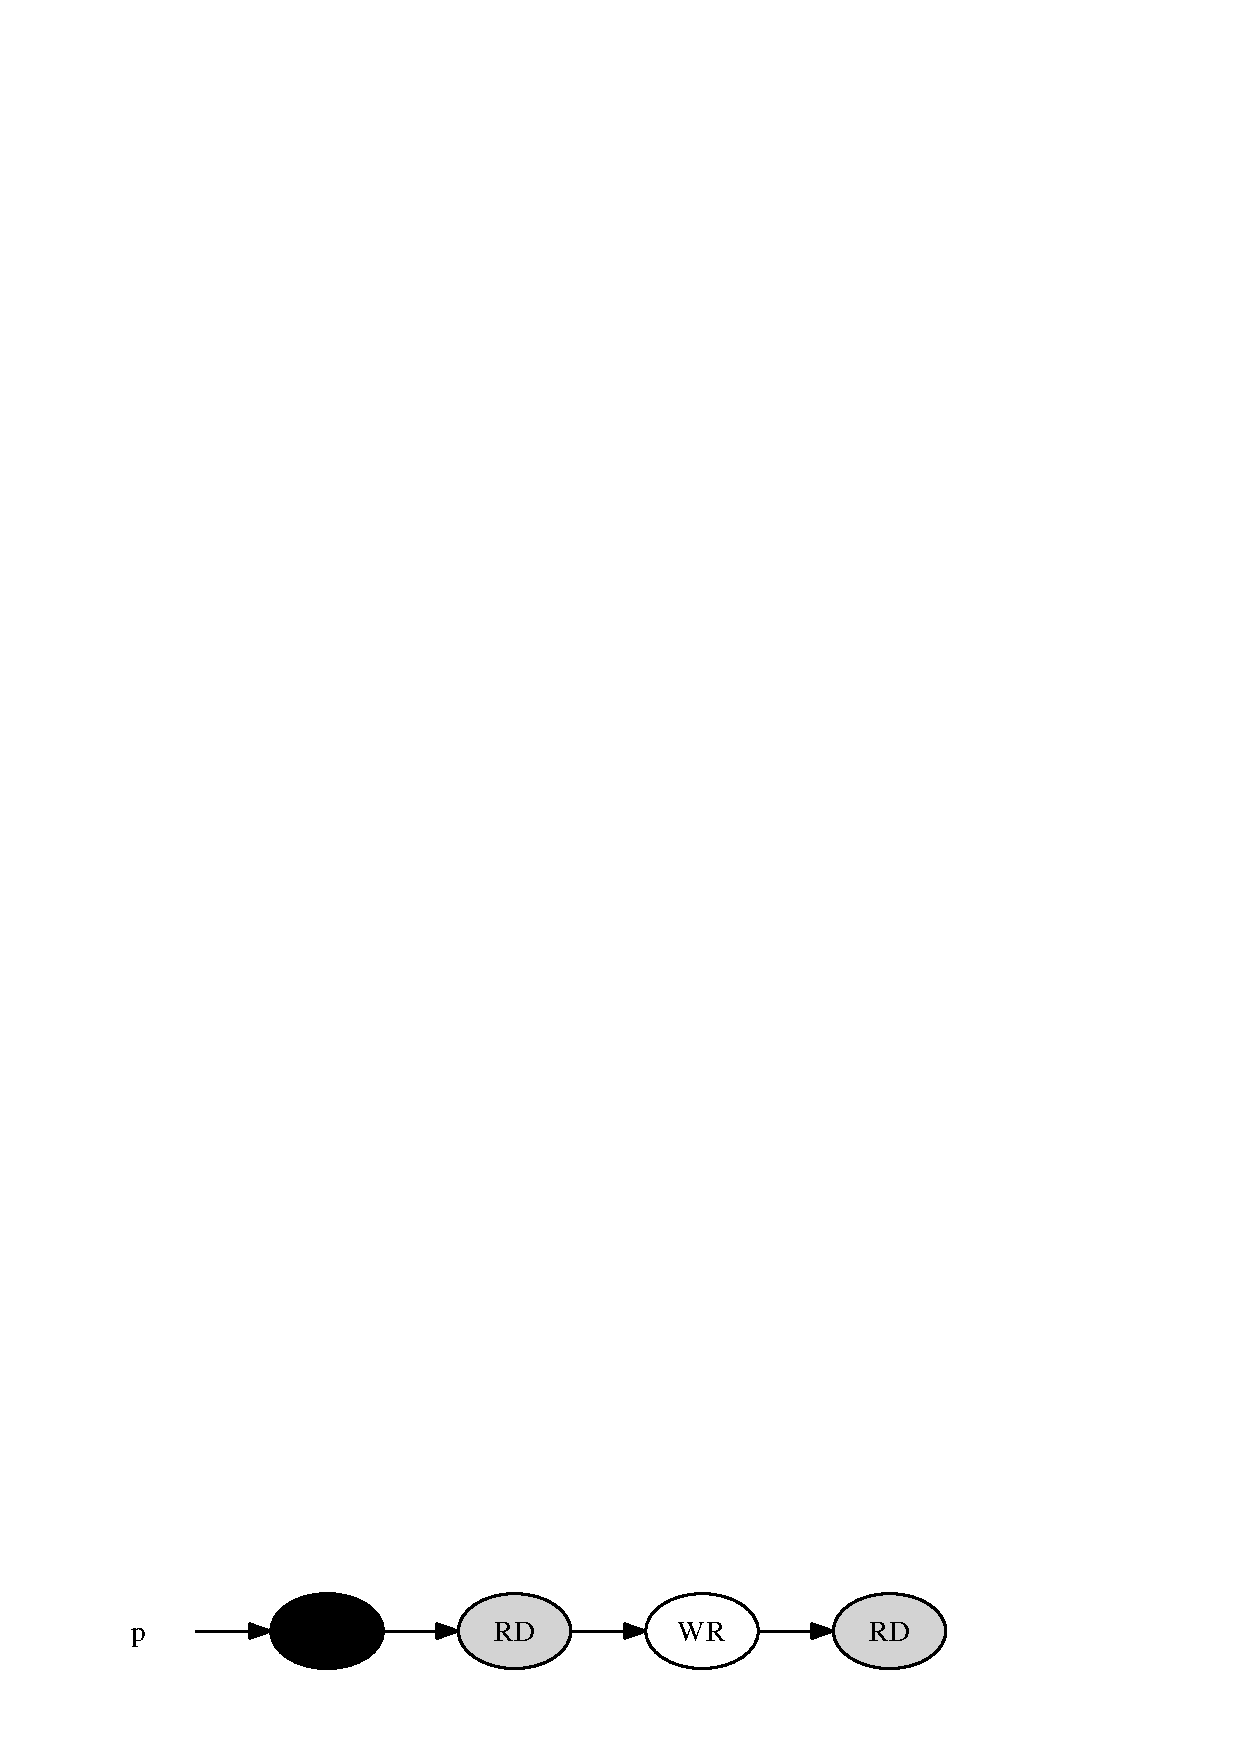
\includegraphics[scale=0.6]{grph_RD_WR} & \\
%      (a) & (b) \\
  %    (a) Nodes read and written by code & 
  %    (b) Code fragment traversing the data structure. \\
  \hline
    \end{tabular}}
  \end{center}
%  \hrule
  \caption{\label{fig:codeCallGraph} Skeleton of a program with procedure calls}
%\hrule
\end{figure}
  
\begin{example}{\rm
Consider the program shown in Figure~\ref{fig:codeCallGraph}. In this example 
procedure \ttf{f} calls procedure \ttf{g} and procedure \ttf{h}, whereas, 
procedure \ttf{h} again calls procedures \ttf{i} and \ttf{j}. Procedure \ttf{g} calls 
procedure \ttf{k} which in turn calls procedure \ttf{g}, resulting in 
indirect recursive procedure calls. Figure~\ref{fig:callgraph}(a) shows the corresponding 
directed call graph. The shadowed cyclic region in the graph indicates recursion 
in the program. The cyclic call graph is then 
transformed into acyclic graph by removing the 
back edge showed as dotted edge. Figure~\ref{fig:callgraph}(b) presents 
corresponding acyclic graph 
with topological order. 
}
\hfill\psframebox{}  \end{example}
%
\section{Computing Abstract Summary}
\label{sec:funcSummary}
For each callee procedure, we need to obtain 
an abstract summary that summarizes the procedure. 
By abstract summary, we mean the \emph{Read} 
and \emph{Write} sets of symbolic heap locations which are accessed 
for reading and writing operations respectively inside the procedure. 
The motivation behind the technique is to summarize effect of called 
procedure for callers, which in turn is used by the callers to summarize effect 
for called procedure. Summaries, thus obtained for 
each procedure are stored in a table for later use. In  
this analysis propagation of summaries 
follows the bottom-up approach. Hence, abstract summary for all the 
procedures are computed following the reverse topological order of nodes in the 
call graph. 
\begin{figure}
  \begin{center}
    \scalebox{.85}{\begin{tabular}{ c c }
     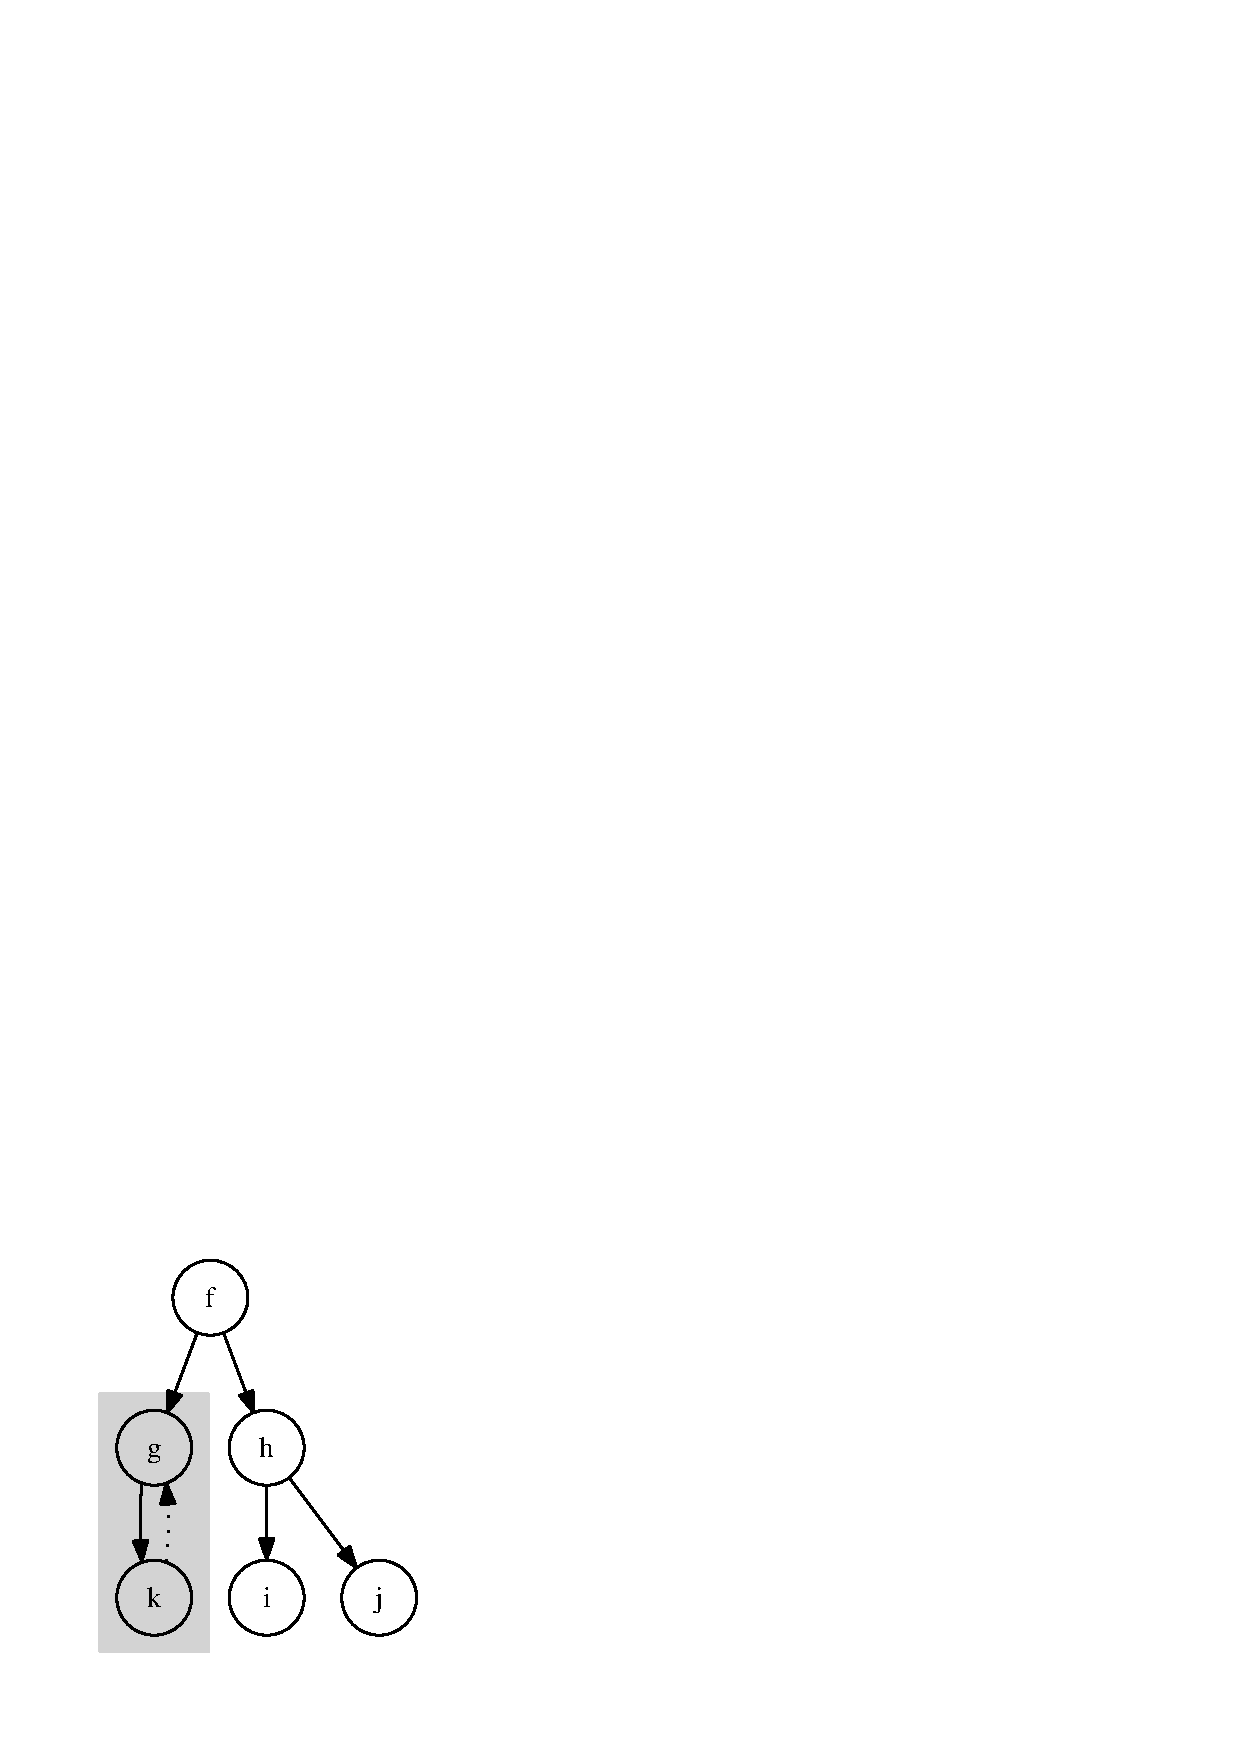
\includegraphics[scale=0.75]{call_graph} %\cline{1-1}
     &
      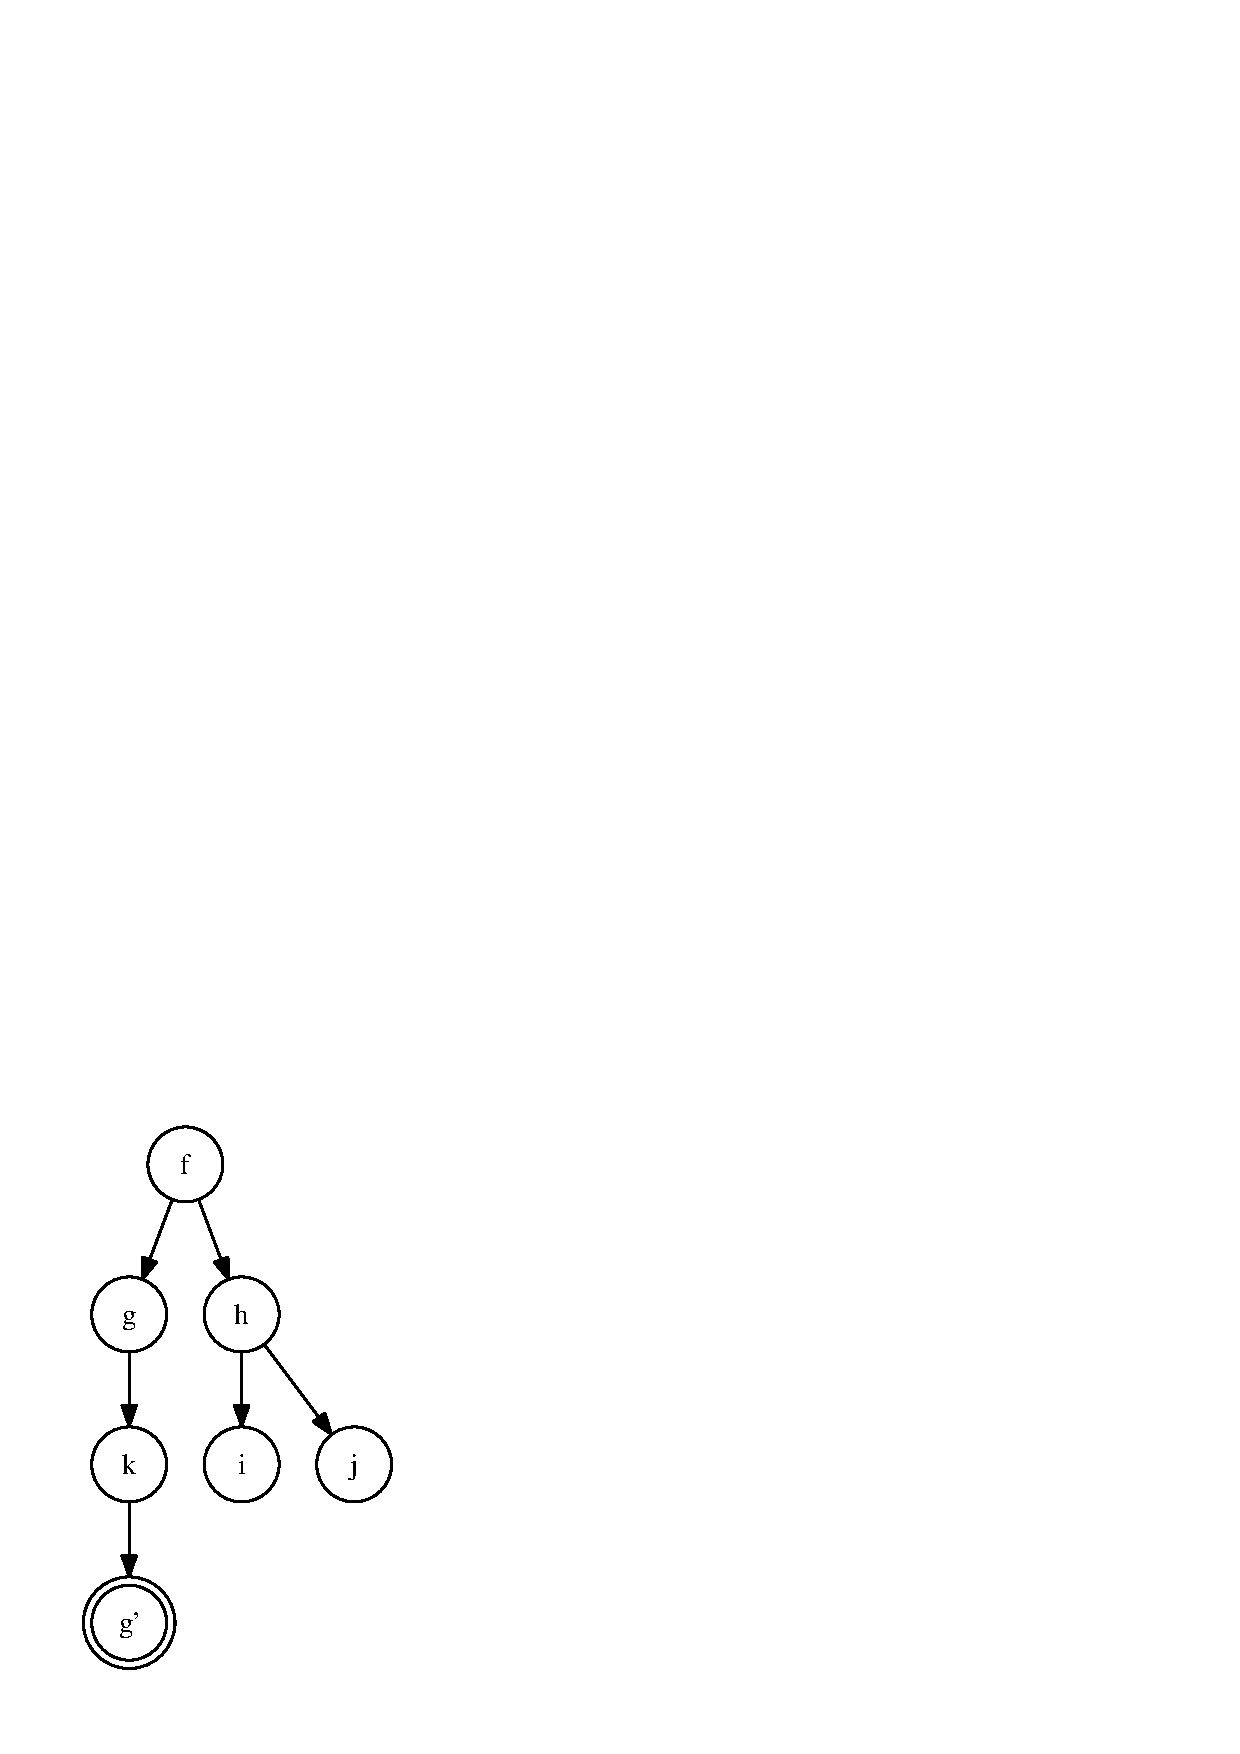
\includegraphics[scale=0.75]{ordered_graph} \\
%      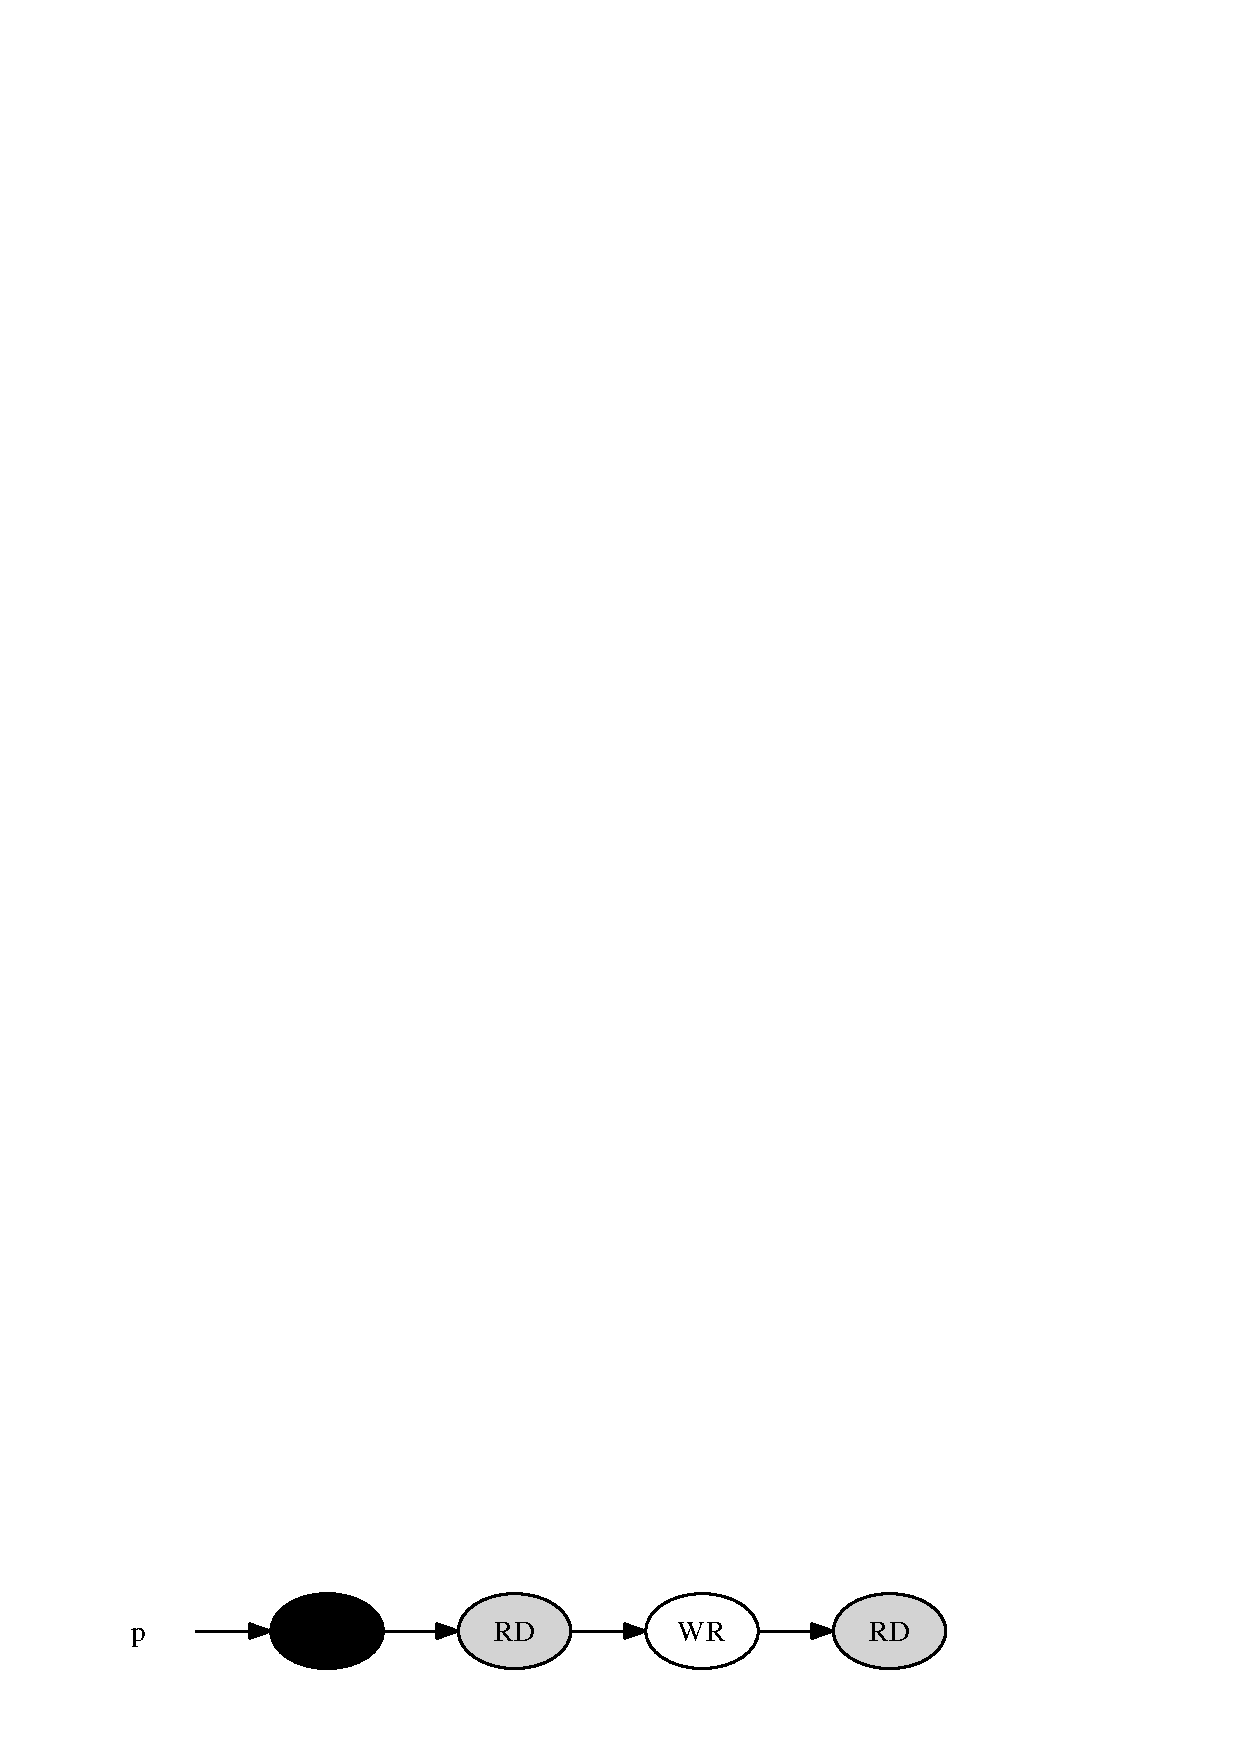
\includegraphics[scale=0.6]{grph_RD_WR} & \\
%      (a) & (b) \\
     (a) Cyclic call graph & 
     (b) Corresponding DAG \\
    \end{tabular}}
  \end{center}
%  \hrule
  \caption{\label{fig:callgraph} Example showing call graph }
%\hrule
\end{figure}
  
All heap directed global  
pointer variables throughout the program are initialized once with proper 
symbolic memory locations. During computation of abstract summary for each  
procedure, the heap directed pointer variables passed as formal 
parameters to the called procedure are 
initialized with random symbolic memory location. As summary, 
our analysis computes read and write sets of access paths with respect 
to the corresponding symbolic memory locations. This process of computation 
follows the intra-procedural analysis as explained before. The same 
procedure is followed by the caller procedure to summarize its effect. 
%
\section{Evaluating Procedure Call}
\label{sec:interProc}
Abstract summary for each callee procedure should be 
used by the caller procedure in the current calling context. 
Summary of each called procedure, thus obtained by intra-procedural analysis, 
contains information in the local context of the procedure.
When the symbolic execution inside the caller function reaches a procedure call, 
the context of the actual parameters is mapped to the respective 
formal parameters of the called procedure. The summary of the callee is 
translated accordingly to be used in the context of caller procedure. 

Summary of a procedure, as mentioned earlier, returns read and write sets 
of paths accessed by corresponding pointer variables. Access paths 
are computed with respect to symbolic memory locations local to the callee  
under analysis. The local symbolic memory locations used in the 
summary of callee are 
mapped into symbolic locations accessed by the caller procedure. 
Such modified summary of caller is used by the callee to summarize its effect. 
Evaluating summary for recursive function does not differ significantly than evaluating non-recursive function. If a recursive function is encountered, the 
analysis will go deep inside the function upto the depth of recursion depending 
upon the precision of analysis. 
\begin{figure}[t]
  \begin{center}
    \scalebox{.85}{\begin{tabular}{ c | c }
%    \hline
	 \multirow{2}{*}{{\tt
\begin{program}{0}
%  \FL\ \ldots
  \NL{0} procedure f(p) 
  \NL{0} begin
  \NL{1}  q = p\rtarrow{next};
  \NL{1}  g(q);
  \NL{0}  end
  \NL{0} procedure g(r)
  \NL{0}  begin
  \NL{1}  $\cdots$ = r\rtarrow{num};
  \NL{1}  s = r\rtarrow{next};
  \NL{1}  s\rtarrow{num}=$\cdots$;
  \NL{0}  end
 \end{program}
 
}} %\cline{1-1}
     & \\
    & 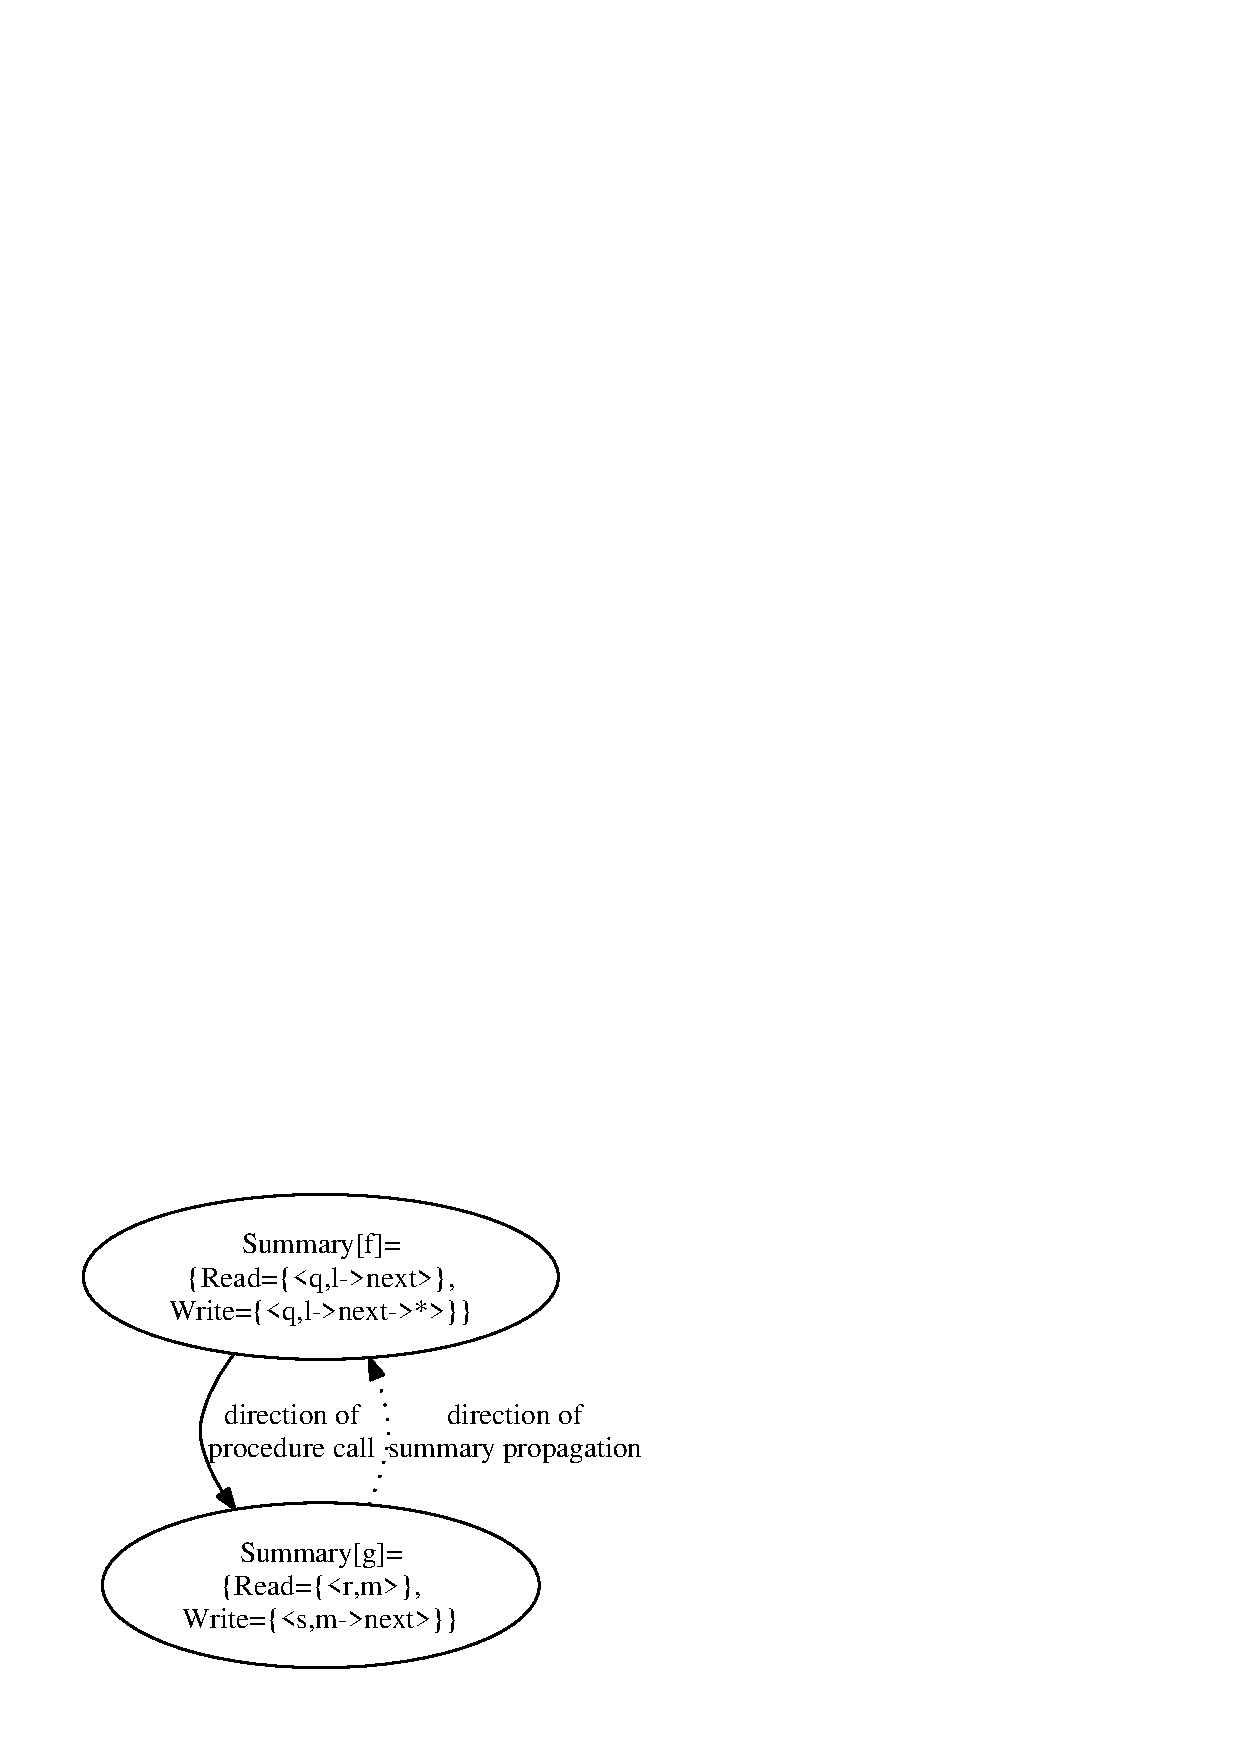
\includegraphics[scale=0.7]{grph5} \\
%      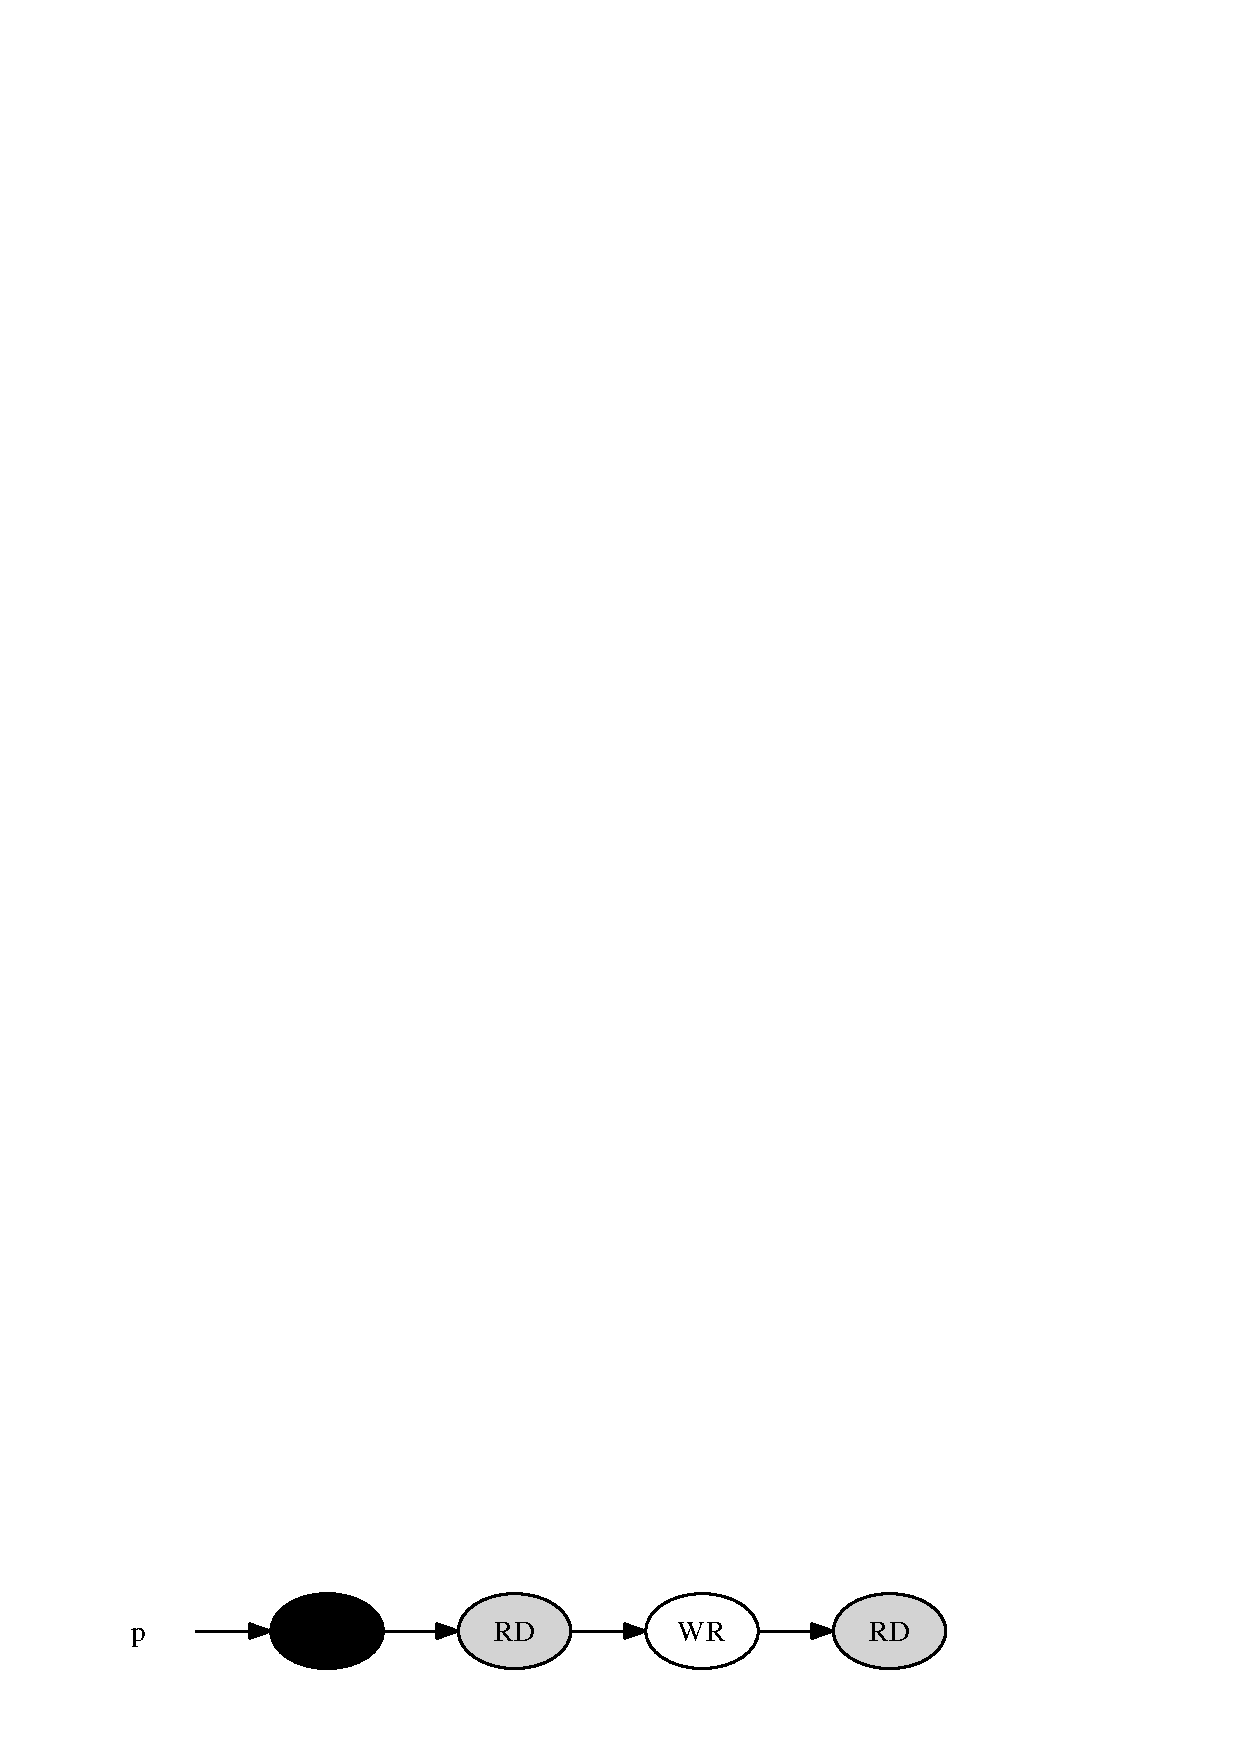
\includegraphics[scale=0.6]{grph_RD_WR} & \\
%     (a) & (b) \\
      (a) Example program with procedure call &
     (b) Call graph showing summary of procedures \\
 %    \hline
%     \hline
    \end{tabular}}
  \end{center}
  \hrule
  \caption{\label{fig:codeInter} Example showing computation of abstract summary}
%\hrule
\end{figure}
\begin{example}{\rm 
Let us consider the example program and the corresponding call graph shown in 
Figure~\ref{fig:codeInter}. In the example program procedure 
\ttf{f} calls procedure \ttf{g}. The solid line in the call graph gives the direction 
for calling subroutines, whereas, the dotted line shows the direction for propagation 
of summary information. Summary information of procedure \ttf{f} and \ttf{g} are also shown in the call graph. At first, summary of procedure \ttf{g} is computed in the 
local context of itself. The summary consists of read and write sets as 
\ttf{\{<r,m>\}} and \ttf{\{<s,m\rtarrow{next}>\}} respectively, where pointer 
variable \ttf{r} is initialized to symbolic memory location \ttf{m}. 
At the call site of procedure \ttf{g}, the actual parameter \ttf{q} takes value 
\ttf{l\rtarrow{next}}, if formal parameter \ttf{p} of procedure \ttf{f} 
points to memory location \ttf{l}. The value of actual parameter \ttf{q} 
modifies the summary of procedure \ttf{g}. This modified summary is further used 
to summarize the information of procedure \ttf{f}. 

}
\hfill\psframebox{}    
\end{example}













\chapter{Experimental Results}
\label{ch:result}
In this chapter we discuss about some experimental results 
of our analysis. We have developed a prototype model of heap 
dependence analysis at two levels: One at the intra-procedural 
level, which works for each procedure separately, and the other 
at the loop level, where the intra-procedural analysis is refined 
in the context of loop. The model is implemented in the Static 
Single Assignment (SSA) intermediate level of GCC (version 4.3.0)
\footnote{Available from http://gcc.gnu.org/}  
framework. The guideline for building and installing GCC from source, with 
newly added pass is given in Appendix A. 
We have conducted experiments over two example programs 
and two benchmark programs. 
The example programs are used to show how our loop-based 
approach successfully detects loop-carried dependences. These 
simple programs are based on single linked-list data structure 
presented in Figure~\ref{ch:loopdep}.3. Other benchmark programs 
\emph{TreeAdd} and \emph{Bisort} are 
drawn from Olden Suite. The prototype model, with manual 
intervention, successfully 
identifies the dependences present in benchmark programs

We have manually pre-processed the programs to be analysed, such that 
the heap accessing statements are normalized into binary statements. 
In the next step, based on type of heap access, the normalized 
statements are tagged accordingly. In the same step informations 
regarding pointers,  used and defined by the statement and the 
pointer field used to access the heap object are attached to 
each statement along with the access type. In the following sections 
we explain the experimental results for intra-procedural analysis 
and loop sensitive analysis.
%%%%%%%%%%%%%%%%%%%%%%%%%%%%%%%%%%%%%%%%%%%%%%%
\begin{figure}
  \begin{center}
    \scalebox{.85}{\begin{tabular}{ c | c }
     {\small \tt
      \begin{tabular}[b]{l}
		{\bf int} treeAdd(tree *t) \{     \\ 
		\ \ \ \ {\bf if} (t == NULL)           \\ 
		\ \ \ \ \ \ \ \ return 0;           \\ 
		\ \ \ \ tl = t$\rightarrow$left;    \\
        \ \ \ \ treeAdd(tl); \\
        \ \ \ \ tr = t$\rightarrow$right; \\
		\ \ \ \ treeAdd(tl); \\
		\ \ \ \ t$\rightarrow${num} = tl$\rightarrow${num} + tr$\rightarrow${num}; \\
		\}
      \end{tabular}
}	  
 %\cline{1-1}
    &
     {\tt
\begin{program}{0}
\UNL{0} int bisort(root,sprval,dir) 
% \FL\ \ldots
\UNL{1} HANDLE *root;
\UNL{1} int sprval, dir;
\UNL{0}\{
\UNL{1}	HANDLE *l;
\UNL{1}	HANDLE *r;
\UNL{1}	 l = root\rtarrow{left};
\UNL{1}      r = root\rtarrow{right};
\UNL{1}      val = root\rtarrow{value};
\UNL{1}     root\rtarrow{value}=bisort(l,val,dir);
\UNL{1}      ndir = !dir;
\UNL{1}      sprval=bisort(r,sprval,ndir);
\UNL{1}      sprval=bimerge(root,sprval,dir);
\UNL{1}    return sprval;
\UNL{0} \} 
  \end{program}
  }
 \\
%      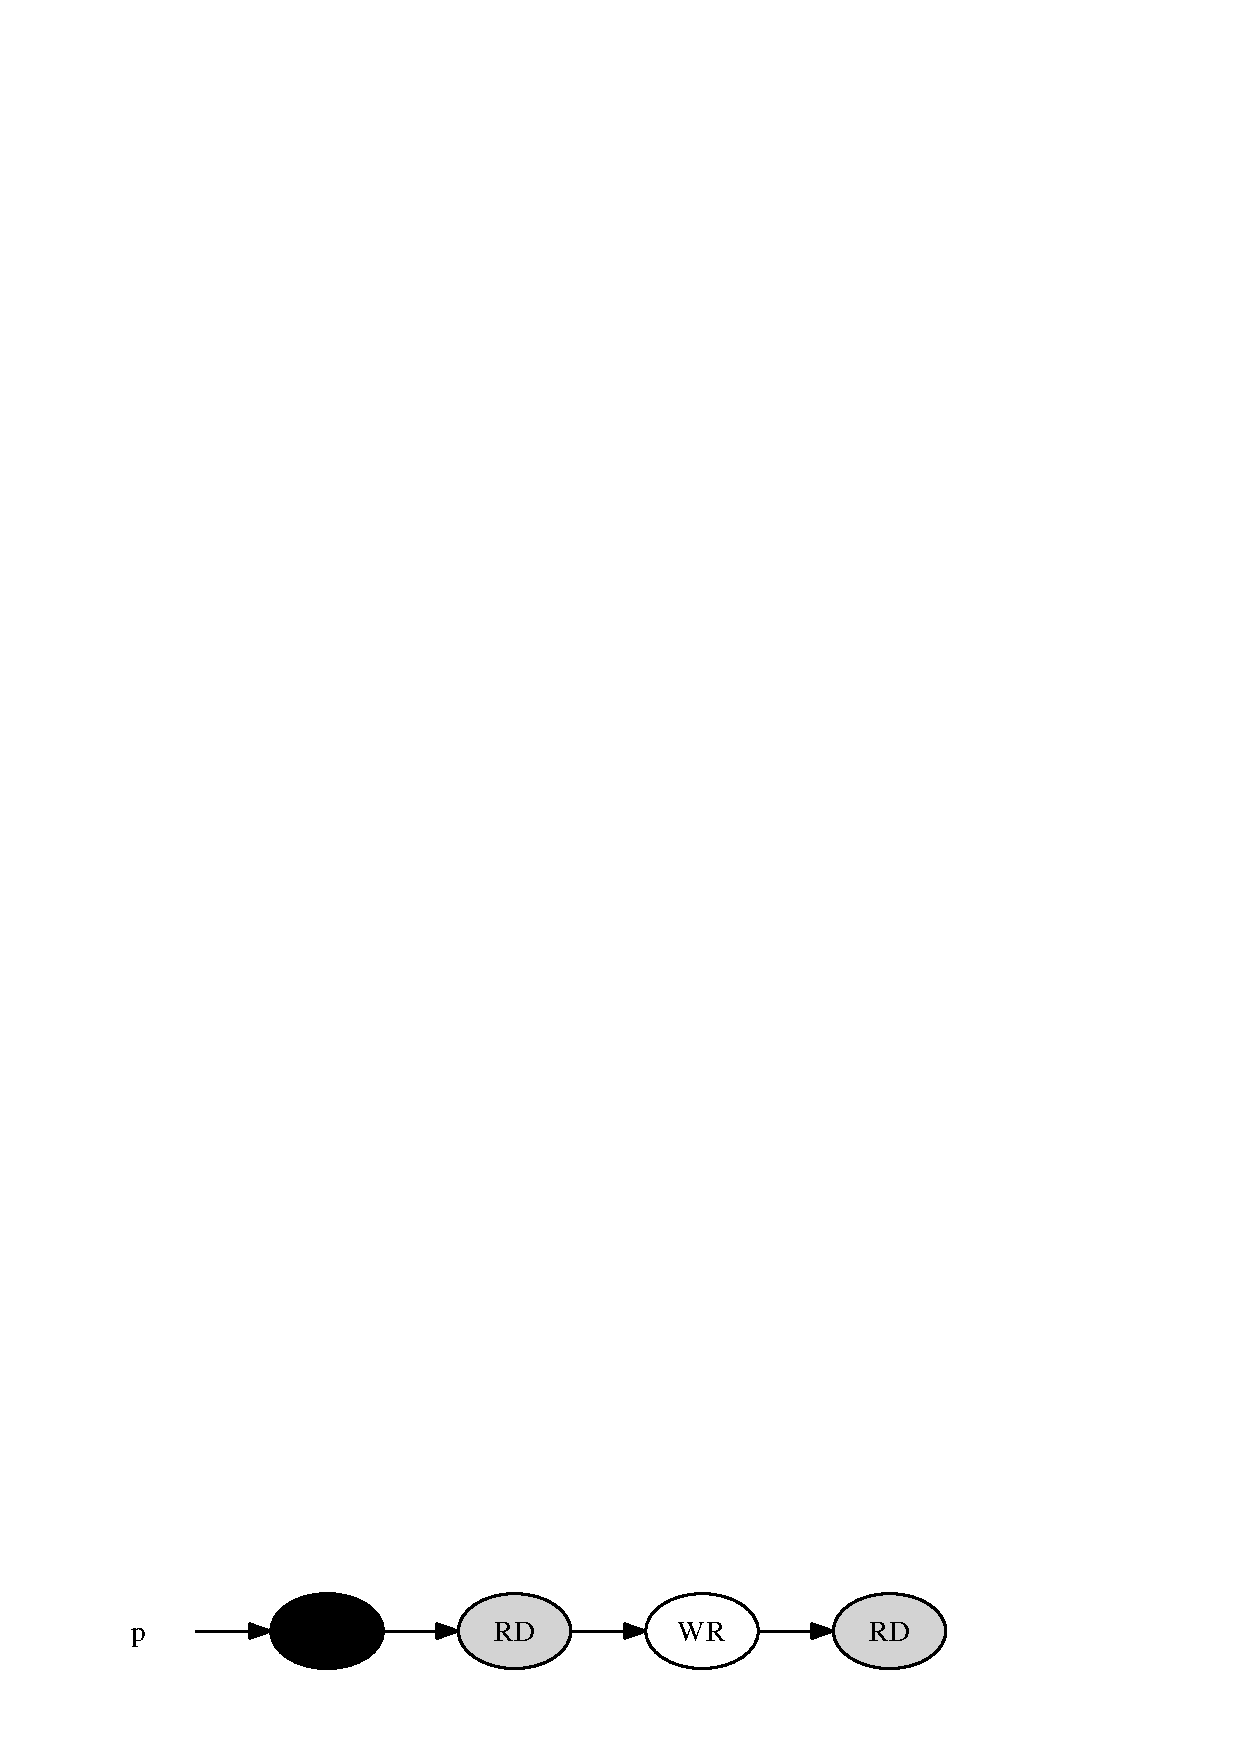
\includegraphics[scale=0.6]{grph_RD_WR} & \\
%     (a) & (b) \\
     (a) Function \emph{treeAdd} & 
      (b) Function \emph{bisort} \\
  \end{tabular}}
  \end{center}
  \hrule
  \caption{\label{fig:bench} Functions of benchmark programs}
%\hrule
\end{figure}
\begin{comment}
\begin{figure}
  \begin{center}
%    \scalebox{.85}{\begin{tabular}{ c c }
%     {\small \tt
      \begin{tabular}[b]{l}
		{\bf int} treeAdd(tree *t) \{     \\ 
		\ \ \ \ {\bf if} (t == NULL)           \\ 
		\ \ \ \ \ \ \ \ return 0;           \\ 
		\ \ \ \ tl = t$\rightarrow$left;    \\
        \ \ \ \ treeAdd(tl); \\
        \ \ \ \ tr = t$\rightarrow$right; \\
		\ \ \ \ treeAdd(tl); \\
		\ \ \ \ t$\rightarrow${num} = tl$\rightarrow${num} + tr$\rightarrow${num}; \\
		\}
      \end{tabular}
}	  
 %\cline{1-1}
%    &
     {\tt
\begin{program}{0}
\UNL{0} int bisort(root,sprval,dir) 
% \FL\ \ldots
\UNL{1} HANDLE *root;
\UNL{1} int sprval, dir;
\UNL{0}\{
\UNL{1}	HANDLE *l;
\UNL{1}	HANDLE *r;
\UNL{1}	 l = root\rtarrow{left};
\UNL{1}      r = root\rtarrow{right};
\UNL{1}      val = root\rtarrow{value};
\UNL{1}     root\rtarrow{value}=bisort(l,val,dir);
\UNL{1}      ndir = !dir;
\UNL{1}      sprval=bisort(r,sprval,ndir);
\UNL{1}      sprval=bimerge(root,sprval,dir);
\UNL{1}    return sprval;
\UNL{0} \} 
  \end{program}
  }
% \\
%      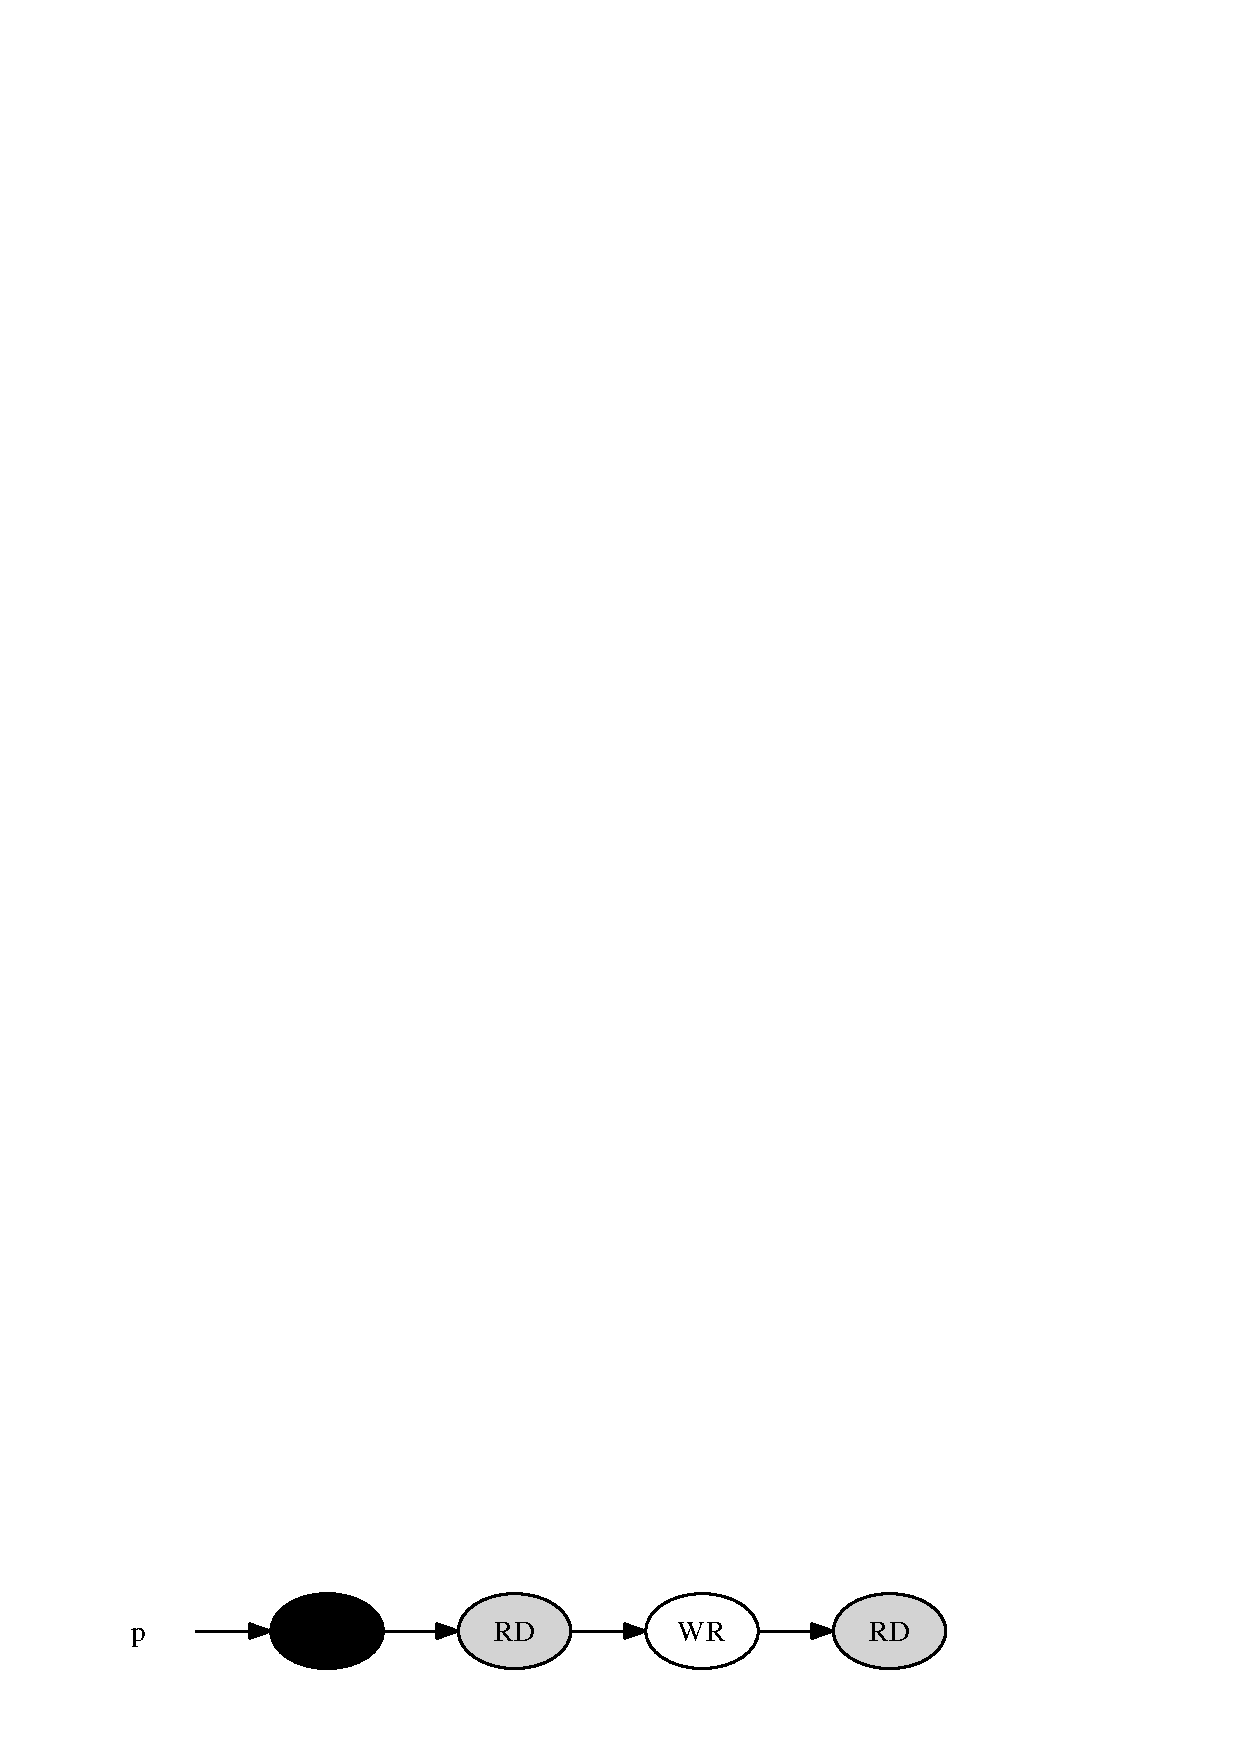
\includegraphics[scale=0.6]{grph_RD_WR} & \\
%      (a) & (b) \\
  %    (a) Nodes read and written by code & 
  %    (b) Code fragment traversing the data structure. \\
%   \end{tabular}}
  \end{center}
%  \hrule
  \caption{\label{fig:bisort} Function \emph{bisort}}
%\hrule
\end{figure}
\end{comment}
\section{Benchmarks}
Benchmark program \emph{TreeAdd} operates on binary tree and recursively adds the 
values of tree. The \emph{treeAdd} function from benchmark 
program \emph{TreeAdd} is analysed. This function  
recursively calls itself to compute values of its left and right subtrees. 
Left and right subtree values, thus computed are added to the value of the 
root to compute the value of whole tree. Figure~\ref{fig:bench}(a)  
shows the function \emph{treeAdd}. 
The main objective behind the analysis is to find out 
whether the recursive function calls on left and write subtrees 
can be executed in parallel. 
The function \emph{bisort} from the benchmark program \emph{Bisort} 
is also analysed to extract function call level parallelism. Function \emph{bisort} 
performs bitonic sort over binary tree by recursively calling itself on left and right subtrees 
of the root. 
The analysis is fine tuned in the context of loops. The experiments for loop sensitive 
dependence analysis are done on example programs \emph{List-1} and \emph{List-2} shown in 
Figure 5.3. Both the programs traverse single-linked list and in each iteration the functions  
read data from the current heap node and write the same data into the next node. But the function \emph{List-1} navigates iterations using two occurrences of pointer field \emph{next}, whereas,  function \emph{List-2} navigates using a single occurrence of \emph{next} pointer field. 
Hence by manual inspection it is clear that function \emph{List-1} does not have any loop  
dependence, but function \emph{List-2} poses loop dependences. 
%%%%%%%%%%%%%%%%%%%%%%%%%%%%%%%%%%%%%%%%%%%%%%%
\section{Results of Intra-Procedural Analysis}
The prototype model for intra-procedural dependence detection 
performs the state analysis which computes the set of pairs, consisting 
of pointer variable and path accessing corresponding symbolic heap location. 
In the next pass over the program, the model successfully computes 
the read and write sets of access paths for each heap accessing 
statement in the program. Next we manually check for each pair 
of heap accessing statements to find out any conflict in terms 
of data access. The interference predicate \ttf{isInterfering}, 
produced by shape analysis returns true if the access paths under 
objection lead to common heap location. 
%%%%%%%%%%%%%%%%%%%%%%%%%%%%%%%%
\begin{table}
\centering
\begin{tabular}{| l | c | c | c |}
\hline 
\bf{Program} & \bf{Traversal pattern} & \bf{Potential Dependence} & \bf{Type of dependence}\tn
\hline \hline
{\tt TreeAdd} & {\tt 2 nested} & {\tt No} & {\tt No dep.}\\
& {\tt rec. function} & & \\
\hline
{\tt Bisort} & {\tt 2 nested} & {\tt No} & {\tt No dep.}\\
& {\tt rec. function} & & \\
\hline
{\tt List-1} & {\tt single loop} & {\tt Yes} & {\tt Anti dep.}\\
\hline
{\tt List-2} & {\tt single loop} & {\tt Yes} & {\tt Anti dep.}\\
\hline
\end{tabular}
\caption{Result of programs tested by intra-procedural analysis} 
\label{fig:tableResutIntra}
%\hrule
\end{table}
%%%%%%%%%%%%%%%%%%%%%%%%%%%%%%%%%%%%%
In the Table~\ref{fig:tableResutIntra} we have given results of 
intra-procedural analysis. It reports no dependence at function 
call level for \emph{treeAdd} and \emph{bisort}. However, 
the analysis reports dependencies of type anti dependence for both  
example programs \emph{List-1} and \emph{List-2}.

%%%%%%%%%%%%%%%%%%%%%%%%%%%%%%%%%%%%%%%%%%%%%%%%%%%%%%%
\section{Results of Loop-Sensitive Analysis}
The basic prototype model identifies navigator variable and 
navigator expression, used by the loop to traverse over the 
data structure. It then computes the full length access paths 
being read or written by each statement within the body of the loop. 
The programs \emph{List-1} and \emph{List-2} are further analysed to refine dependence analysis. 
The previous analysis detects spurious dependencies in case of loop. 
Both example programs work on 
single linked list, which is of type Tree. As there exists no 
sharing within the underlying data structure, the generalized 
equations, formed by the access paths, are tested for loop-carried 
dependencies. Lamport test successfully reports no dependence for 
function \emph{List-1} and dependence of type 
anti dependence for function \emph{List-2}. 
\epsfig{file=certificate.ps,bbllx=0pt,bblly=0pt,bburx=594pt,bbury=842pt,width=10cm,angle=90}





% \section{Conclusion}

In this report we have suggested several enhancements to Sandeep's work on Field Sensitive analysis
which ensure the correctness and increase the accuracy of the analysis.
Now after these changes the analysis is better than Ghiya's work in all those unit test cases described. 
We have also introduced a new analysis called subset based analysis which infers shape based on the subset of fields actually accessed inside
a function. This helps us inferring information like a function is traversing/accessing a tree substructure of a cyclic data structure. 
We also proposed a shape sensitive inter procedural
analysis which is in mid way of context sensitive and context insensitive analysis and could possibly balance the memory consumption and 
preciseness at the same time. We have also performed various 
optimizations with the aim of decreasing the memory consumption and time for completion.
The testing strategy used is exhaustive and has helped a lot in identifying the cases of safe and incorrect results.

There are some benchmarks where the results are not as good as Ghiya's, these are due to the
summarization of heap nodes due to the dummy statement. In the future we plan to work on
this issue.
The analysis has concerns over the amount of memory it takes even after the optimizations performed. We want
to address this concern by representing boolean equations in much efficient way. 
% The callstring approach is using
% more memory for this analysis, so we plan to find out some other context sensitive analysis which is
% memory efficient.

% \section{Future Work}
% Representation of boolean equations in a memory efficient
% Better memory efficient Context sensitive analysis
% Extend this for arrays of pointers



\appendix
\chapter{Guideline for Adding New Pass in GCC}
\subsubsection*{Pre-requisities for Configuring GCC-4.3.0}
\begin{enumerate}
\item GMP-4.3.2 and MPFR-2.4.1 should be installed.
\item Build GMP and MPFR in \$GMPBUILD and \$MPFRBUILD directory respectively.
\end{enumerate}
%%%%%%%%%%%%%%%%%%%%%%%%%%%%%%%%%%%%%%%%%%%%%%%%%%%%%%%
\subsubsection*{How to Configure and Build GCC}
\begin{enumerate}
\item Let \$SOURCEDIR be the source directory for GCC and \$HOME be the home directory where \$SOURCEDIR is present.
\item Create another directory \$BUILDDIR in \$HOME and follow the following steps.
\item	cd \$BUILDDIR
\item	../\$SOURCEDIR/configure --enable-languages=c \\
--with-gmp=/home/user/\$GMPBUILD --with-mpfr=/home/user/\$MPFRBUILD
\item make
\item make install
\item make all-gcc TARGET-gcc=/home/\$BUILDDIR/gcc/cc1
\end{enumerate}
%%%%%%%%%%%%%%%%%%%%%%%%%%%%%%%%%%%%%%%%%%%%%%%%%%%%%%%%%%
\subsubsection*{How to Register Pass in GIMPLE SSA level in GCC}
\begin{enumerate}
\item Place the new file named \emph{tree-loop-distribution.c} in \$SOURCEDIR/gcc/.
\item Adding the pass in pass hierarchy : Add NEXT\_PASS (pass\_loop\_distribution); after NEXT\_PASS(pass\_linear\_transform); in file passes.c
\item Add extern struct tree\_opt\_pass pass\_loop\_distribution; in file named tree-pass.h
\item Add the following lines in file named common.opt\\
ftree-loop-distribution\\
Common Report Var(flag\_tree\_loop\_distribution)\\
Enable loop distribution on trees
\item Add DEFTIMEVAR (TV\_TREE\_LOOP\_DISTRIBUTION, ``tree loop distributio'') after DEFTIMEVAR (TV\_TREE\_LINEAR\_TRANSFORM, ``tree loop linear'') in file timevar.def
\item Edit Makefile.in : Add following rules
tree-loop-distribution.o \  \\
tree-loop-distribution.o : tree-loop-distribution.c \$(CONFIG\_H) \ \\
\$(SYSTEM\_H) coretypes.h \$(TM\_H) \$(GCC\_H) \$(OPTABS\_H) \ \\
\$(TREE\_H) \$(RTL\_H) \$(BASIC\_BLOCK\_H) \$(DIAGONSTIC\_H) \ \\
\$(TREE\_FLOW\_H) \$(TREE\_DUMP\_H) \$(TIMEVAR\_H) \$(CFGLOOP\_H) \ \\
tree-pass.h \$(TREE\_DATA\_REF\_H) \$(SCEV\_H) \$(EXPR\_H) \$(TARGET\_H) \ \\
tree-chrec.h 
\item make
\item make install
\end{enumerate}

\subsubsection*{Test}
\begin{enumerate}
\item gcc -O -ftree-loop-distribution -fdump-tree-ldist test.c
\item Results dump file named test.c.103t.ldist
\end{enumerate}

%\input{ref.tex}

%\bibliography{Reference}
%\nocite{*}
\bibliographystyle{alpha}
\bibliography{Report}
\end{document}


